\section*{Appendix}\label{appendix}

\setcounter{page}{1}

\subsection{Network Architectures}
The following section includes graphical representations of NN referenced throughout the thesis. %TODO: briefly describe the kindf of archs shown in this section...

\subsubsection{Classifiers}\label{appendix_classifiers}
The graphical representations of the network architectures are created with the tool \textit{visual keras}, by Paul Gavrikov (\cite{Gavrikov2020VisualKeras}).

\begin{figure}[htbp]
    \centering
    \vspace{-.5em}
    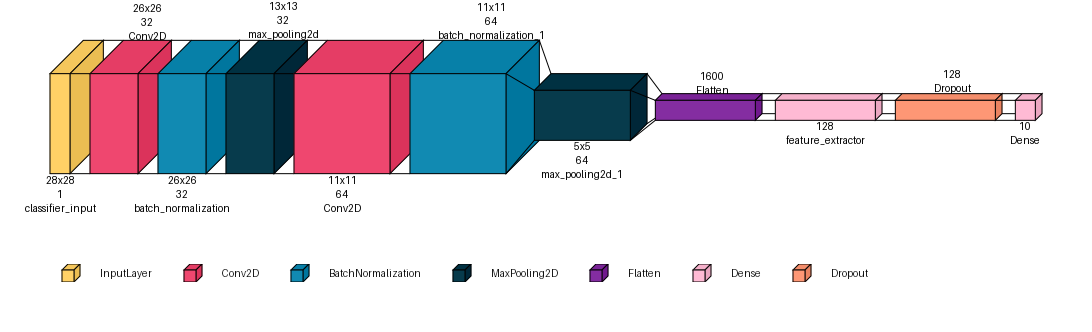
\includegraphics[width=.9\textwidth]{abb/netron_network_archs/classifying_Classifier_MNIST.png}
    \caption{Depiction of the CNN architecture used to classify unlabeled images from the MNIST GDA experiments and judge the effectiveness of said GDA. (Image created with \cite{Gavrikov2020VisualKeras})}
    \label{fig:figure_class_mnist}
\end{figure}

\begin{figure}[htbp]
    \centering
    \vspace{-2em}
    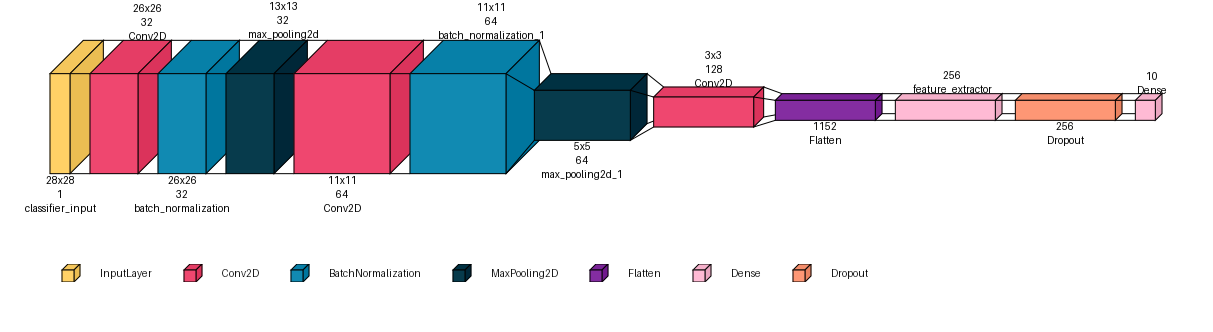
\includegraphics[width=.9\textwidth]{abb/netron_network_archs/classifying_Classifier_FashionMNIST.png}
    \caption{Depiction of the CNN architecture used to classify unlabeled images from the Fashion-MNIST GDA experiments and judge the effectiveness of said GDA. (Image created with \cite{Gavrikov2020VisualKeras})}
    \label{fig:figure_class_fashion}
\end{figure}

\begin{figure}[htbp]
    \centering
    \vspace{-2em}
    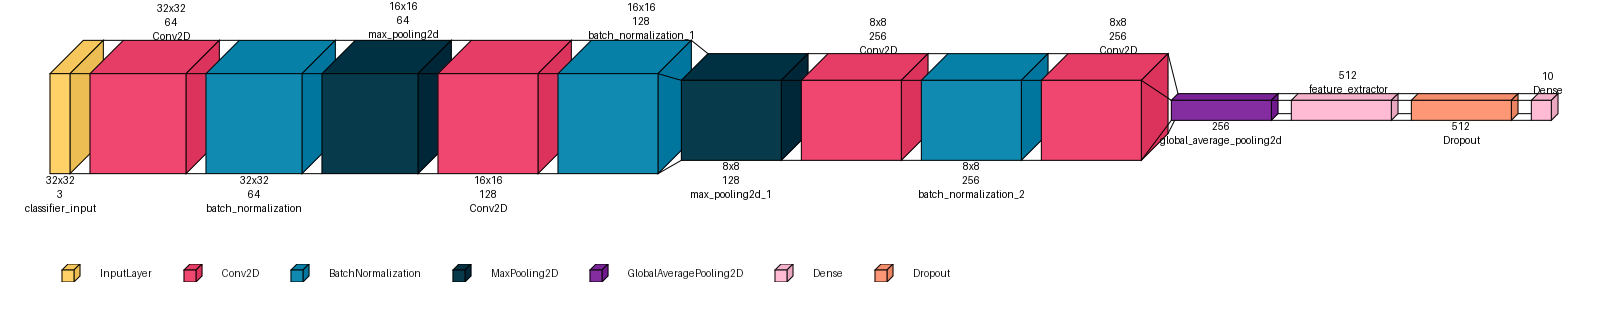
\includegraphics[width=.9\textwidth]{abb/netron_network_archs/classifying_Classifier_Cifar10.png}
    \caption{Depiction of the CNN architecture used to classify unlabeled images from the CIFAR10 GDA experiments and judge the effectiveness of said GDA. (Image created with \cite{Gavrikov2020VisualKeras})}
    \label{fig:figure_class_cifar10}
\end{figure}
\newpage

\subsubsection{Generator Model Architectures}\label{appendix_generator_architectures}
The graphical representations of the network architectures are created with the tool \textit{visual keras}, by Paul Gavrikov (\cite{Gavrikov2020VisualKeras}).

\begin{figure}[htbp]
    \centering
    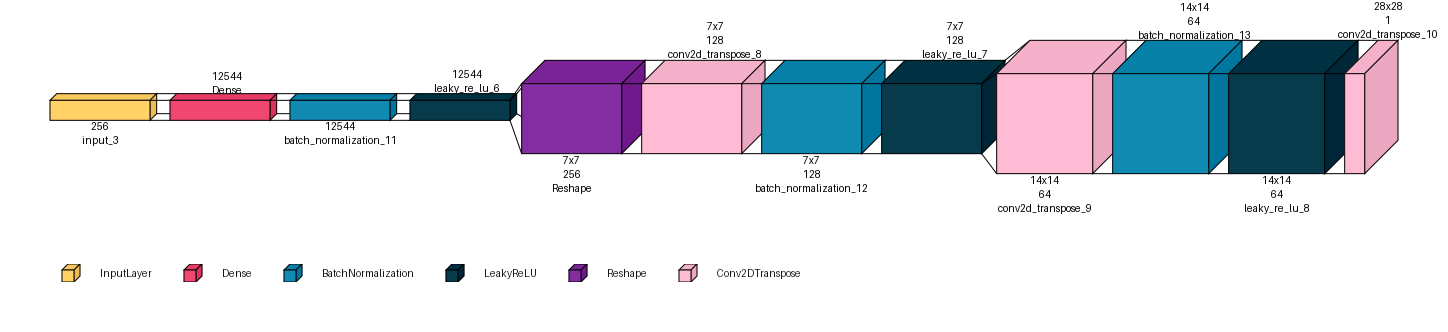
\includegraphics[width=.9\textwidth]{abb/netron_network_archs/define_vanilla_mnist_gen.png}
    \caption{Depiction of the generator used in the deep convolutional GAN dependent experiments. Used to train a generator and create fake image data based on the MNIST dataset.}
    \label{fig:figure_gen_arch_vanilla_mnist}
\end{figure}

\begin{figure}[htbp]
    \centering
    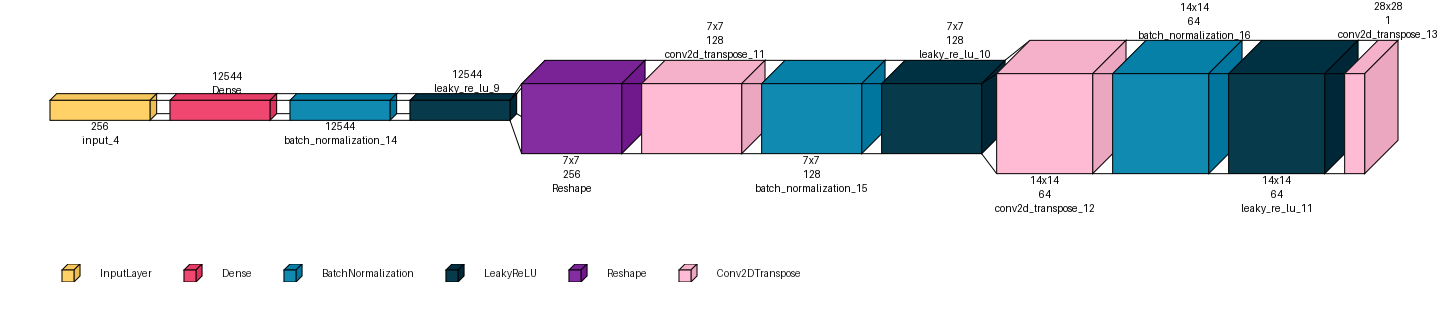
\includegraphics[width=.9\textwidth]{abb/netron_network_archs/define_vanilla_fashion_mnist_gen.png}
    \caption{Depiction of the generator used in the deep convolutional GAN dependent experiments. Used to train a generator and create fake image data based on the Fashion-MNIST dataset.}
    \label{fig:figure_gen_arch_vanilla_fashion}
\end{figure}

\begin{figure}[htbp]
    \centering
    \vspace{-2em}
    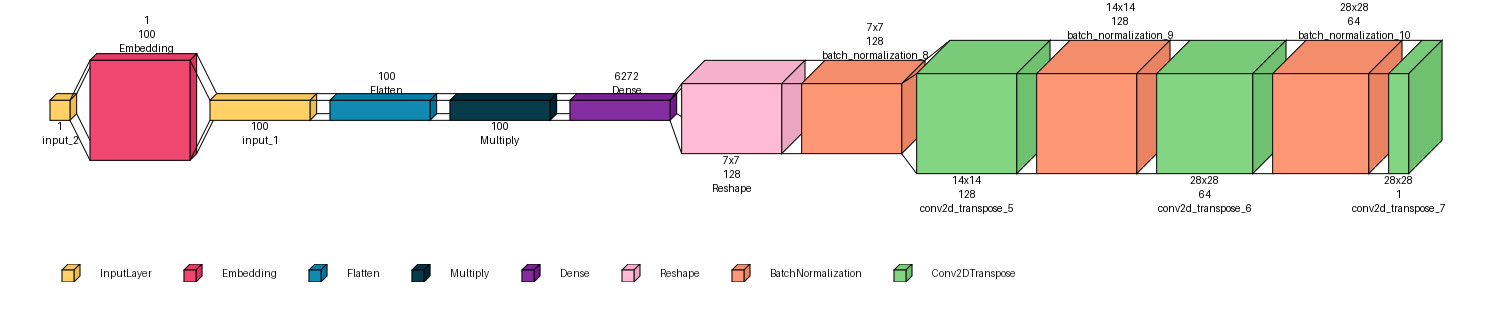
\includegraphics[width=.9\textwidth]{abb/netron_network_archs/define_conditional_mnists_gen.png}
    \caption{Depiction of the generator used in the Conditional GAN dependent experiments. Used to train a generator and create fake image data based on the MNIST and Fashion-MNIST datasets.}
    \label{fig:figure_gen_arch_conditional}
\end{figure}

\begin{figure}[htbp]
    \centering
    \vspace{-2em}
    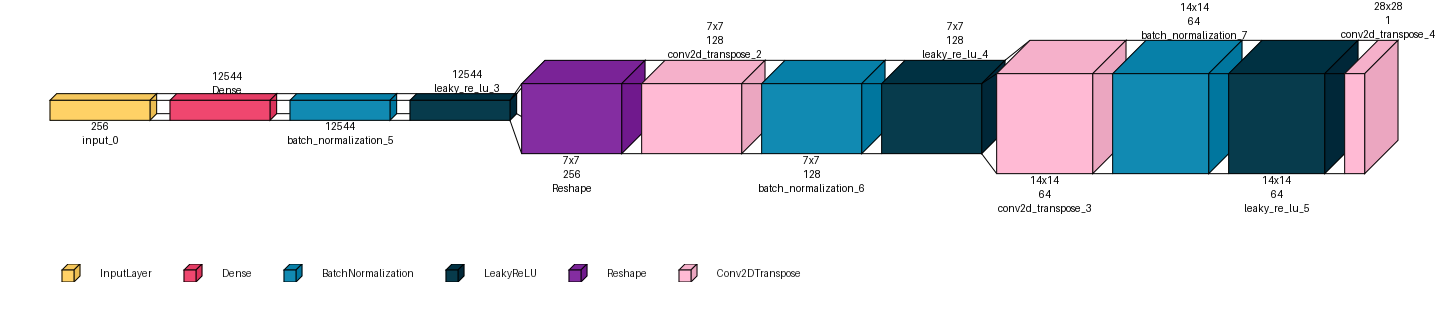
\includegraphics[width=.9\textwidth]{abb/netron_network_archs/define_madgan_mnists_gen.png}
    \caption{Depiction of the generators used in the MADGAN dependent experiments. Used to train a generator and create fake image data based on the MNIST and Fashion-MNIST datasets.}
    \label{fig:figure_gen_arch_madgan}
\end{figure}

\begin{figure}[htbp]
    \centering
    \vspace{-2em}
    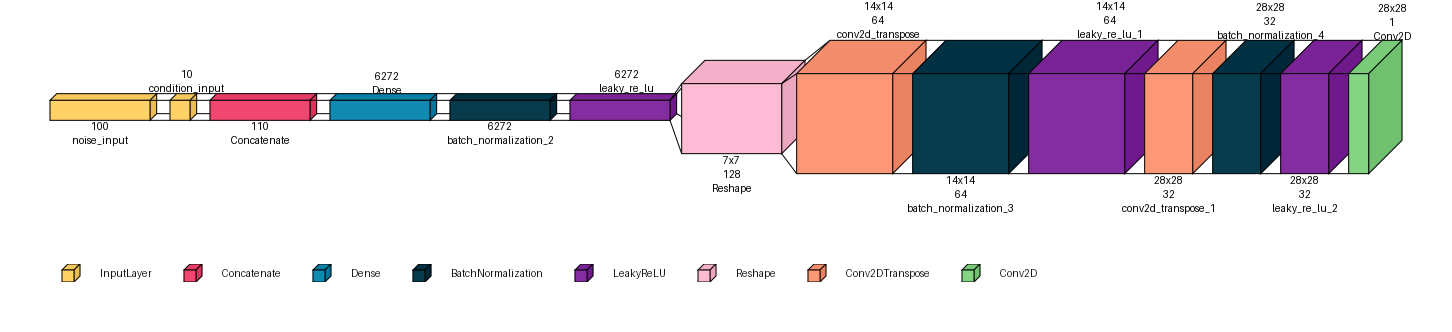
\includegraphics[width=.9\textwidth]{abb/netron_network_archs/define_cmadgan_mnists_gen.png}
    \caption{Depiction of the generators used in the cMADGAN dependent experiments. Used to train a generator and create fake image data based on the MNIST and Fashion-MNIST datasets.}
    \label{fig:figure_gen_arch_cmadgan}
\end{figure}
\newpage


\subsubsection{Discriminator Model Architectures}\label{appendix_discriminator_architectures}
The graphical representations of the network architectures are created with the tool \textit{visual keras}, by Paul Gavrikov (\cite{Gavrikov2020VisualKeras}).

\begin{figure}[htbp]
    \centering
    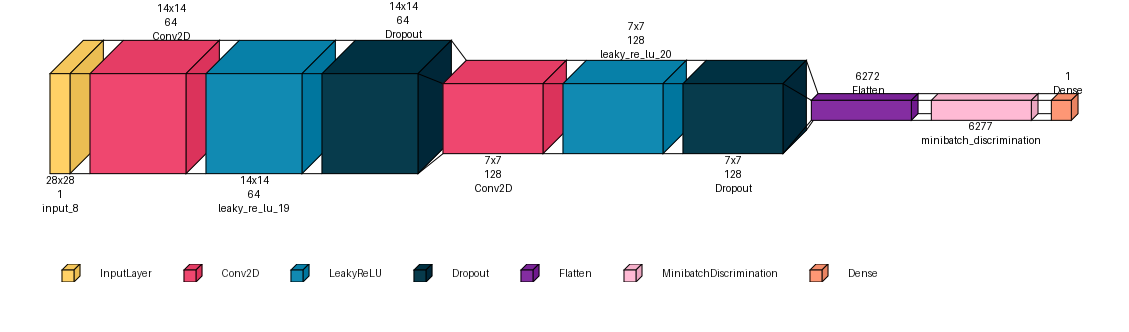
\includegraphics[width=.9\textwidth]{abb/netron_network_archs/define_vanilla_mnist_disc.png}
    \caption{Depiction of the discriminator used in the deep convolutional GAN dependent experiments. Used to train a generator based on the MNIST dataset.}
    \label{fig:figure_disc_arch_vanilla_mnist}
\end{figure}

\begin{figure}[htbp]
    \centering
    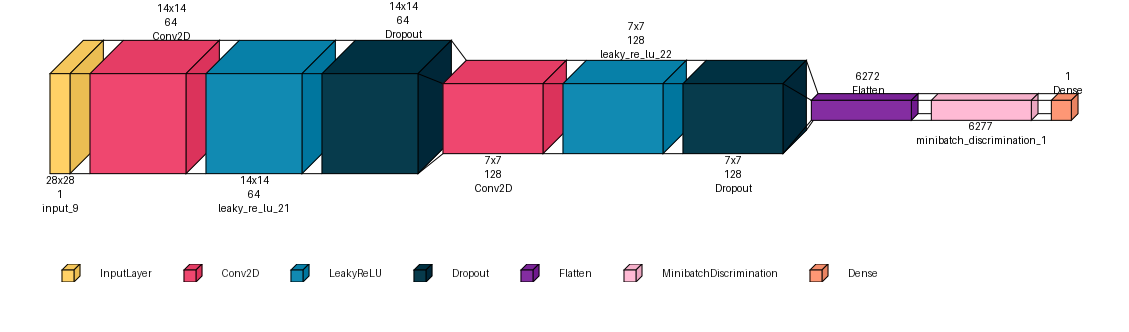
\includegraphics[width=.9\textwidth]{abb/netron_network_archs/define_vanilla_fashion_mnist_disc.png}
    \caption{Depiction of the discriminator used in the deep convolutional GAN dependent experiments. Used to train a generator based on the Fashion-MNIST dataset.}
    \label{fig:figure_disc_arch_vanilla_fashion}
\end{figure}

\begin{figure}[htbp]
    \centering
    \vspace{-2em}
    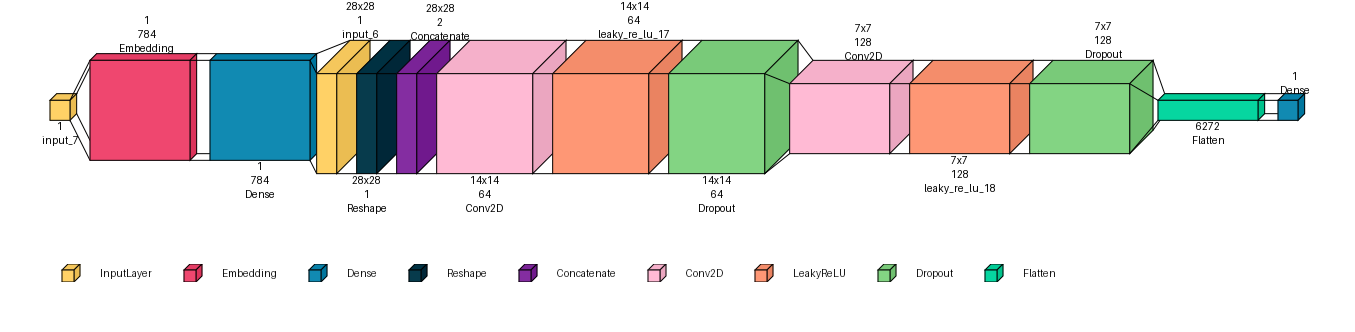
\includegraphics[width=.9\textwidth]{abb/netron_network_archs/define_conditional_mnists_disc.png}
    \caption{Depiction of the discriminator used in the Conditional GAN dependent experiments. Used to train a generator based on the MNIST and Fashion-MNIST datasets.}
    \label{fig:figure_disc_arch_conditional}
\end{figure}

\begin{figure}[htbp]
    \centering
    \vspace{-2em}
    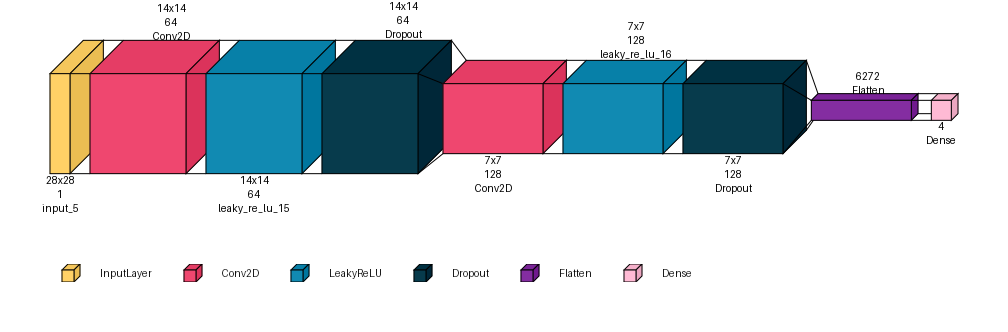
\includegraphics[width=.9\textwidth]{abb/netron_network_archs/define_madgan_mnists_disc.png}
    \caption{Depiction of the discriminator used in the MADGAN dependent experiments. Used to train a generator based on the MNIST and Fashion-MNIST datasets.}
    \label{fig:figure_disc_arch_madgan}
\end{figure}

\begin{figure}[htbp]
    \centering
    \vspace{-2em}
    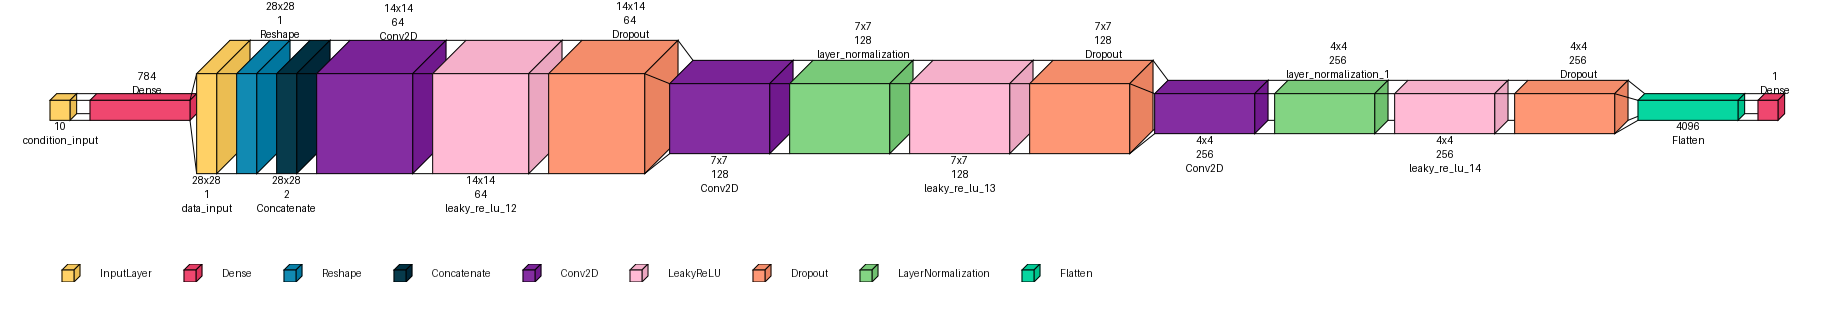
\includegraphics[width=.9\textwidth]{abb/netron_network_archs/define_cmadgan_mnists_disc.png}
    \caption{Depiction of the discriminator used in the cMADGAN dependent experiments. Used to train a generator based on the MNIST and Fashion-MNIST datasets.}
    \label{fig:figure_disc_arch_cmadgan}
\end{figure}

\newpage


\subsection{FID and Inception Scores from MADGAN Architectures}

\subsubsection{MADGAN MNIST}
\begin{table}[H]
    \centering
    \begin{tabular}{|c|c|c|c|c|}
    \hline
    N Generators & Index & FID & IS & IS-std \\
    \hline
    \textit{Baseline} & & $-0.004$ & $2.549$ & $0.036$ \\
    \specialrule{.1em}{.05em}{.05em}
    & 0 &        $23.597$ & $2.519$ & $0.050$ \\
    3 & 1 &      $22.682$ & $2.506$ & $0.027$ \\
    & 2 &        $23.252$ & $2.509$ & $0.045$ \\
    \hline
    & 0 &        $23.304$ & $2.467$ & $0.030$ \\
    & 1 &        $22.020$ & $2.446$ & $0.040$ \\
    5 & 2 &      $23.076$ & $2.497$ & $0.046$ \\
    & 3 &        $22.265$ & $2.467$ & $0.060$ \\
    & 4 &        $22.614$ & $2.479$ & $0.045$ \\
    \hline
    & 0 &        $22.487$ & $2.513$ & $0.031$ \\
    & 1 &        $21.076$ & $\mathbf{2.548}$ & $0.087$ \\
    & 2 &        $20.941$ & $2.530$ & $0.056$ \\
    7 & 3 &      $22.250$ & $2.520$ & $0.035$ \\
    & 4 &        $21.557$ & $2.530$ & $0.051$ \\
    & 5 &        $21.297$ & $2.545$ & $0.035$ \\
    & 6 &        $21.582$ & $2.541$ & $0.059$ \\
    \hline
    & 0 &        $21.338$ & $2.456$ & $0.045$ \\
    & 1 &        $20.872$ & $2.462$ & $0.040$ \\
    & 2 &        $20.680$ & $2.477$ & $0.028$ \\
    & 3 &        $21.315$ & $2.470$ & $0.030$ \\
    10 & 4 &     $21.158$ & $2.484$ & $0.027$ \\
    & 5 &        $20.655$ & $2.473$ & $0.037$ \\
    & 6 &        $21.090$ & $2.452$ & $0.039$ \\
    & 7 &        $20.689$ & $2.508$ & $0.048$ \\
    & 8 &        $21.471$ & $2.480$ & $0.044$ \\
    & 9 &        $\mathbf{20.459}$ & $2.477$ & $0.036$ \\
    \hline
\end{tabular}
\caption{Effect of varying the number of generators ($N=3, 5, 7, 10$) in the MADGAN model on FID and Inception Score (IS $\pm$ Std. Dev) for the \textbf{MNIST} dataset. Results for each generator index are presented alongside baseline metrics.}
\label{tab:app_madgan_mnist_fid_is}
\end{table}
\newpage


\subsubsection{MADGAN Fashion-MNIST}
\begin{table}[H]
    \centering
    \begin{tabular}{|c|c|c|c|c|}
    \hline
    N Generators & Index & FID & IS & IS-std \\
    \hline
    \textit{Baseline} & & $-0.004$ & $4.723$ & $0.056$ \\
    \specialrule{.1em}{.05em}{.05em}
    & 0 &       $26.086$ & $4.463$ & $0.103$ \\
    3 & 1 &     $25.884$ & $4.487$ & $0.099$ \\
    & 2 &       $26.637$ & $4.538$ & $0.094$ \\
    \hline
    & 0 &       $23.393$ & $4.467$ & $0.119$ \\
    & 1 &       $24.756$ & $4.520$ & $0.107$ \\
    5 & 2 &     $25.663$ & $4.506$ & $0.123$ \\
    & 3 &       $23.614$ & $4.487$ & $0.082$ \\
    & 4 &       $23.665$ & $4.504$ & $0.061$ \\
    \hline
    & 0 &       $22.370$ & $4.558$ & $0.111$ \\
    & 1 &       $21.838$ & $4.536$ & $0.087$ \\
    & 2 &       $21.923$ & $4.508$ & $0.101$ \\
    7 & 3 &     $25.403$ & $4.517$ & $0.112$ \\
    & 4 &       $31.493$ & $4.372$ & $0.087$ \\
    & 5 &       $22.158$ & $4.595$ & $0.075$ \\
    & 6 &       $21.942$ & $4.577$ & $0.087$ \\
    \hline
    & 0 &       $22.454$ & $4.534$ & $0.117$ \\
    & 1 &       $21.914$ & $4.524$ & $0.121$ \\
    & 2 &       $21.327$ & $4.494$ & $0.089$ \\
    & 3 &       $21.630$ & $4.455$ & $0.063$ \\
    10 & 4 &    $\mathbf{20.851}$ & $\mathbf{4.575}$ & $0.097$ \\
    & 5 &       $21.268$ & $4.561$ & $0.048$ \\
    & 6 &       $22.324$ & $4.566$ & $0.127$ \\
    & 7 &       $21.633$ & $4.542$ & $0.084$ \\
    & 8 &       $21.503$ & $4.533$ & $0.127$ \\
    & 9 &       $20.963$ & $4.552$ & $0.100$ \\
    \hline
    \end{tabular}
    \caption{Effect of varying the number of generators ($N=3, 5, 7, 10$) in the MADGAN model on FID and Inception Score (IS $\pm$ Std. Dev) for the \textbf{Fashion-MNIST} dataset. Results for each generator index are presented alongside baseline metrics.}
    \label{tab:madgan_fasion_mnist_fid_is}
\end{table}
\newpage

\subsubsection{cMADGAN MNIST}
\begin{table}[H]
    \centering
    \begin{tabular}{|c|c|c|c|c|}
    \hline
    N Generators & Index & FID & IS & IS-std \\
    \hline
    \textit{Baseline} & & $-0.004$ & $2.549$ & $0.036$ \\
    \specialrule{.1em}{.05em}{.05em}
    & 0 &       $30.105$ & $\mathbf{2.494}$ & $0.034$ \\
    3 & 1 &     $23.875$ & $2.317$ & $0.041$ \\
    & 2 &       $\mathbf{22.753}$ & $2.384$ & $0.032$ \\
    \hline
    & 0 &       $37.638$ & $2.460$ & $0.039$ \\
    & 1 &       $26.614$ & $2.378$ & $0.052$ \\
    5 & 2 &     $26.739$ & $2.356$ & $0.025$ \\
    & 3 &       $27.642$ & $2.309$ & $0.034$ \\
    & 4 &       $26.722$ & $2.246$ & $0.043$ \\
    \hline
    & 0 &       $23.141$ & $2.418$ & $0.037$ \\
    & 1 &       $28.071$ & $2.363$ & $0.036$ \\
    & 2 &       $33.490$ & $2.340$ & $0.033$ \\
    7 & 3 &     $28.333$ & $2.347$ & $0.031$ \\
    & 4 &       $35.599$ & $2.296$ & $0.050$ \\
    & 5 &       $36.075$ & $2.389$ & $0.047$ \\
    & 6 &       $29.807$ & $2.326$ & $0.036$ \\
    \hline
    & 0 &       $108.079$ & $2.076$ & $0.011$ \\
    & 1 &       $82.478$ & $2.250$ & $0.022$ \\
    & 2 &       $153.369$ & $2.124$ & $0.023$ \\
    & 3 &       $126.574$ & $1.846$ & $0.005$ \\
    10 & 4 &    $110.012$ & $2.005$ & $0.013$ \\
    & 5 &       $130.054$ & $1.861$ & $0.009$ \\
    & 6 &       $103.016$ & $2.010$ & $0.011$ \\
    & 7 &       $74.926$ & $2.383$ & $0.035$ \\
    & 8 &       $110.265$ & $2.086$ & $0.014$ \\
    & 9 &       $106.762$ & $1.975$ & $0.033$ \\
    \hline
    \end{tabular}
    \caption{Effect of varying the number of generators ($N=3, 5, 7, 10$) in the cMADGAN model on FID and Inception Score (IS $\pm$ Std. Dev) for the \textbf{MNIST} dataset. Results for each generator index are presented alongside baseline metrics.}
    \label{tab:cmadgan_mnist_fid_is}
\end{table}
\newpage

\subsubsection{cMADGAN Fashion-MNIST}
\begin{table}[H]
    \centering
    \begin{tabular}{|c|c|c|c|c|}
    \hline
    N Generators & Index & FID & IS & IS-std \\
    \hline
    \textit{Baseline} & & $-0.004$ & $4.723$ & $0.056$ \\
    \specialrule{.1em}{.05em}{.05em}
    & 0 &       $25.874$ & $4.750$ & $0.132$ \\
    3 & 1 &     $27.235$ & $4.068$ & $0.090$ \\
    & 2 &       $\mathbf{23.556}$ & $\mathbf{5.049}$ & $0.093$ \\
    \hline
    & 0 &       $170.120$ & $2.938$ & $0.020$ \\
    & 1 &       $167.446$ & $3.430$ & $0.052$ \\
    5 & 2 &     $221.934$ & $3.325$ & $0.032$ \\
    & 3 &       $187.293$ & $3.269$ & $0.029$ \\
    & 4 &       $53.616$ & $3.770$ & $0.057$ \\
    \hline
    & 0 &       $156.601$ & $2.392$ & $0.016$ \\
    & 1 &       $172.054$ & $3.325$ & $0.033$ \\
    & 2 &       $171.505$ & $2.754$ & $0.024$ \\
    7 & 3 &     $97.514$ & $3.273$ & $0.058$ \\
    & 4 &       $155.474$ & $3.157$ & $0.063$ \\
    & 5 &       $151.494$ & $2.623$ & $0.018$ \\
    & 6 &       $174.161$ & $2.976$ & $0.028$ \\
    \hline
    & 0 &       $147.670$ & $3.650$ & $0.037$ \\
    & 1 &       $167.407$ & $2.816$ & $0.026$ \\
    & 2 &       $109.349$ & $3.914$ & $0.068$ \\
    & 3 &       $160.305$ & $3.674$ & $0.040$ \\
    10 & 4 &    $181.778$ & $2.961$ & $0.023$ \\
    & 5 &       $154.633$ & $3.297$ & $0.022$ \\
    & 6 &       $166.511$ & $2.759$ & $0.034$ \\
    & 7 &       $156.135$ & $3.173$ & $0.027$ \\
    & 8 &       $155.758$ & $3.853$ & $0.036$ \\
    & 9 &       $191.126$ & $3.073$ & $0.034$ \\
    \hline
    \end{tabular}
    \caption{Effect of varying the number of generators ($N=3, 5, 7, 10$) in the cMADGAN model on FID and Inception Score (IS $\pm$ Std. Dev) for the \textbf{Fashion-MNIST} dataset. Results for each generator index are presented alongside baseline metrics.}
    \label{tab:cmadgan_fashnion_mnist_fid_is}
\end{table}
\newpage


\subsubsection{DCGAN MNIST}
\begin{table}[H]
    \centering
    \begin{tabular}{|c|c|c|c|}
    \hline
    N Generators & FID & IS & IS-std \\
    \hline
    \textit{Baseline} & $-0.004$ & $2.549$ & $0.036$ \\
    \specialrule{.1em}{.05em}{.05em}
    1 & $122.097$ & $2.611$ & $0.056$ \\
    \hline
    \end{tabular}
    \caption{FID and Inception Score (Mean $\pm$ Std. Dev) for a single DCGAN generator ($N=1$) trained on the \textbf{MNIST} dataset. Baseline scores are included for reference.}
    \label{tab:dcgan_mnist_n1}
\end{table}

\subsubsection{DCGAN Fashion-MNIST}
\begin{table}[H]
    \centering
    \begin{tabular}{|c|c|c|c|}
    \hline
    N Generators & FID & IS & IS-std \\
    \hline
    \textit{Baseline} & $-0.004$ & $4.723$ & $0.056$ \\
    \specialrule{.1em}{.05em}{.05em}
    1 & $123.349$ & $3.573$ & $0.117$ \\
    \hline
    \end{tabular}
    \caption{FID and Inception Score (Mean $\pm$ Std. Dev) for a single DCGAN generator ($N=1$) trained on the \textbf{Fashion-MNIST} dataset. Baseline scores are included for reference.}
    \label{tab:dcgan_fashion_mnist_n1}
\end{table}

\subsubsection{Conditional MNIST}
\begin{table}[H]
    \centering
    \begin{tabular}{|c|c|c|c|}
    \hline
    N Generators & FID & IS & IS-std \\
    \hline
    \textit{Baseline} & $-0.004$ & $2.549$ & $0.036$ \\
    \specialrule{.1em}{.05em}{.05em}
    1 & $28.721$ & $2.553$ & $0.022$ \\
    \hline
    \end{tabular}
    \caption{FID and Inception Score (Mean $\pm$ Std. Dev) for a single Conditional GAN generator ($N=1$) trained on the \textbf{MNIST} dataset. Baseline scores are included for reference.}
    \label{tab:cgan_mnist_n1}
\end{table}

\subsubsection{Conditional Fashion-MNIST}
\begin{table}[H]
    \centering
    \begin{tabular}{|c|c|c|c|}
    \hline
    N Generators & FID & IS & IS-std \\
    \hline
    \textit{Baseline} & $-0.004$ & $4.723$ & $0.056$ \\
    \specialrule{.1em}{.05em}{.05em}
    1 & $25.560$ & $4.210$ & $0.099$ \\
    \hline
    \end{tabular}
    \caption{FID and Inception Score (Mean $\pm$ Std. Dev) for a single Conditional GAN generator ($N=1$) trained on the \textbf{Fashion-MNIST} dataset. Baseline scores are included for reference.}
    \label{tab:cgan_fashion_mnist_n1}
\end{table}

\newpage

\subsection{Stratified Classifier Performances and Graphs} \label{app_strat_class_performance}

\subsubsection{Dataset: MNIST, Architecture: MADGAN}\label{app_strat_class_performance_madgan_mnist}
% LaTeX Metrics Table for Expansion Experiment: - Metric: val_f1_score - Target Gen Group: 3
\noindent\textbf{Expansion Experiment: K=3}
\begin{figure}[htbp]
	\centering
	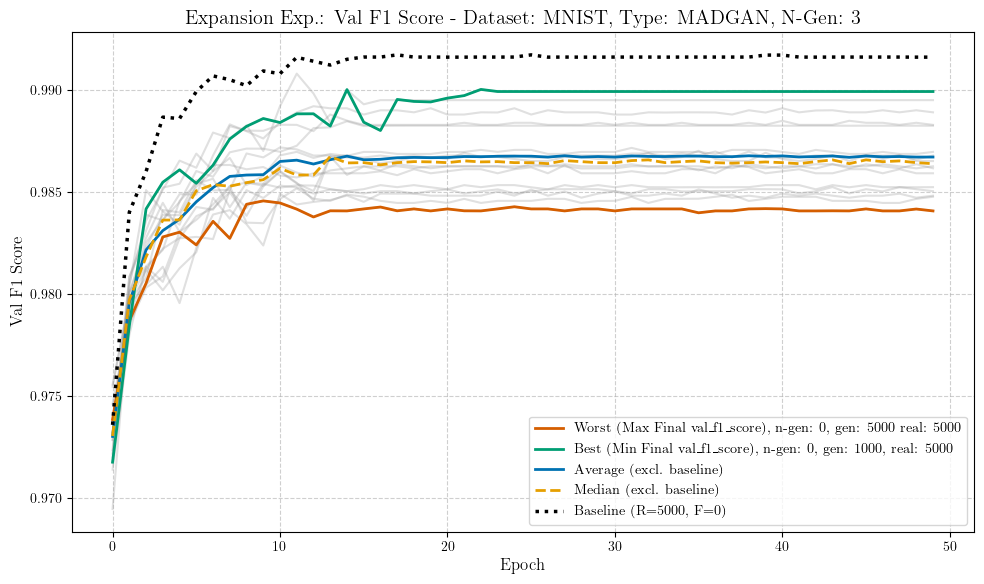
\includegraphics[width=.85\textwidth]{abb/strat_classifier_performance/MNIST_STRATIFIED_CLASSIFIERS_MADGAN_NEW/expansion_experiments/val_f1_score_MADGAN_MNIST_n_gen_3_all.png}
	\label{fig:app_strat_class_performance_expansion_exp._val_f1_score_3}
\end{figure}
\begin{table}[H]
	\vspace{-1.5em}
	\centering
	\begin{tabular}{|c|c|c|c|}
		\hline
		Run Type & Experiment & Val F1 \\ \hline
		best & \(G_{3, 0}\), R:5000, F:1000 & $0.9899$\\ \hline
		worst & \(G_{3, 0}\), R:5000, F:5000 & $0.9841$\\ \hline
		median & G (K=3) & $0.9864$\\ \hline
		average & G (K=3) & $0.9867$
		\\ \hline
	\end{tabular}
\end{table}
% End LaTeX Table for Expansion Experiment:
% LaTeX Metrics Table for Replacement Experiment: - Metric: val_f1_score - Target Gen Group: 3
\noindent\textbf{Replacement Experiment: K=3}
\begin{figure}[htbp]
	\centering
	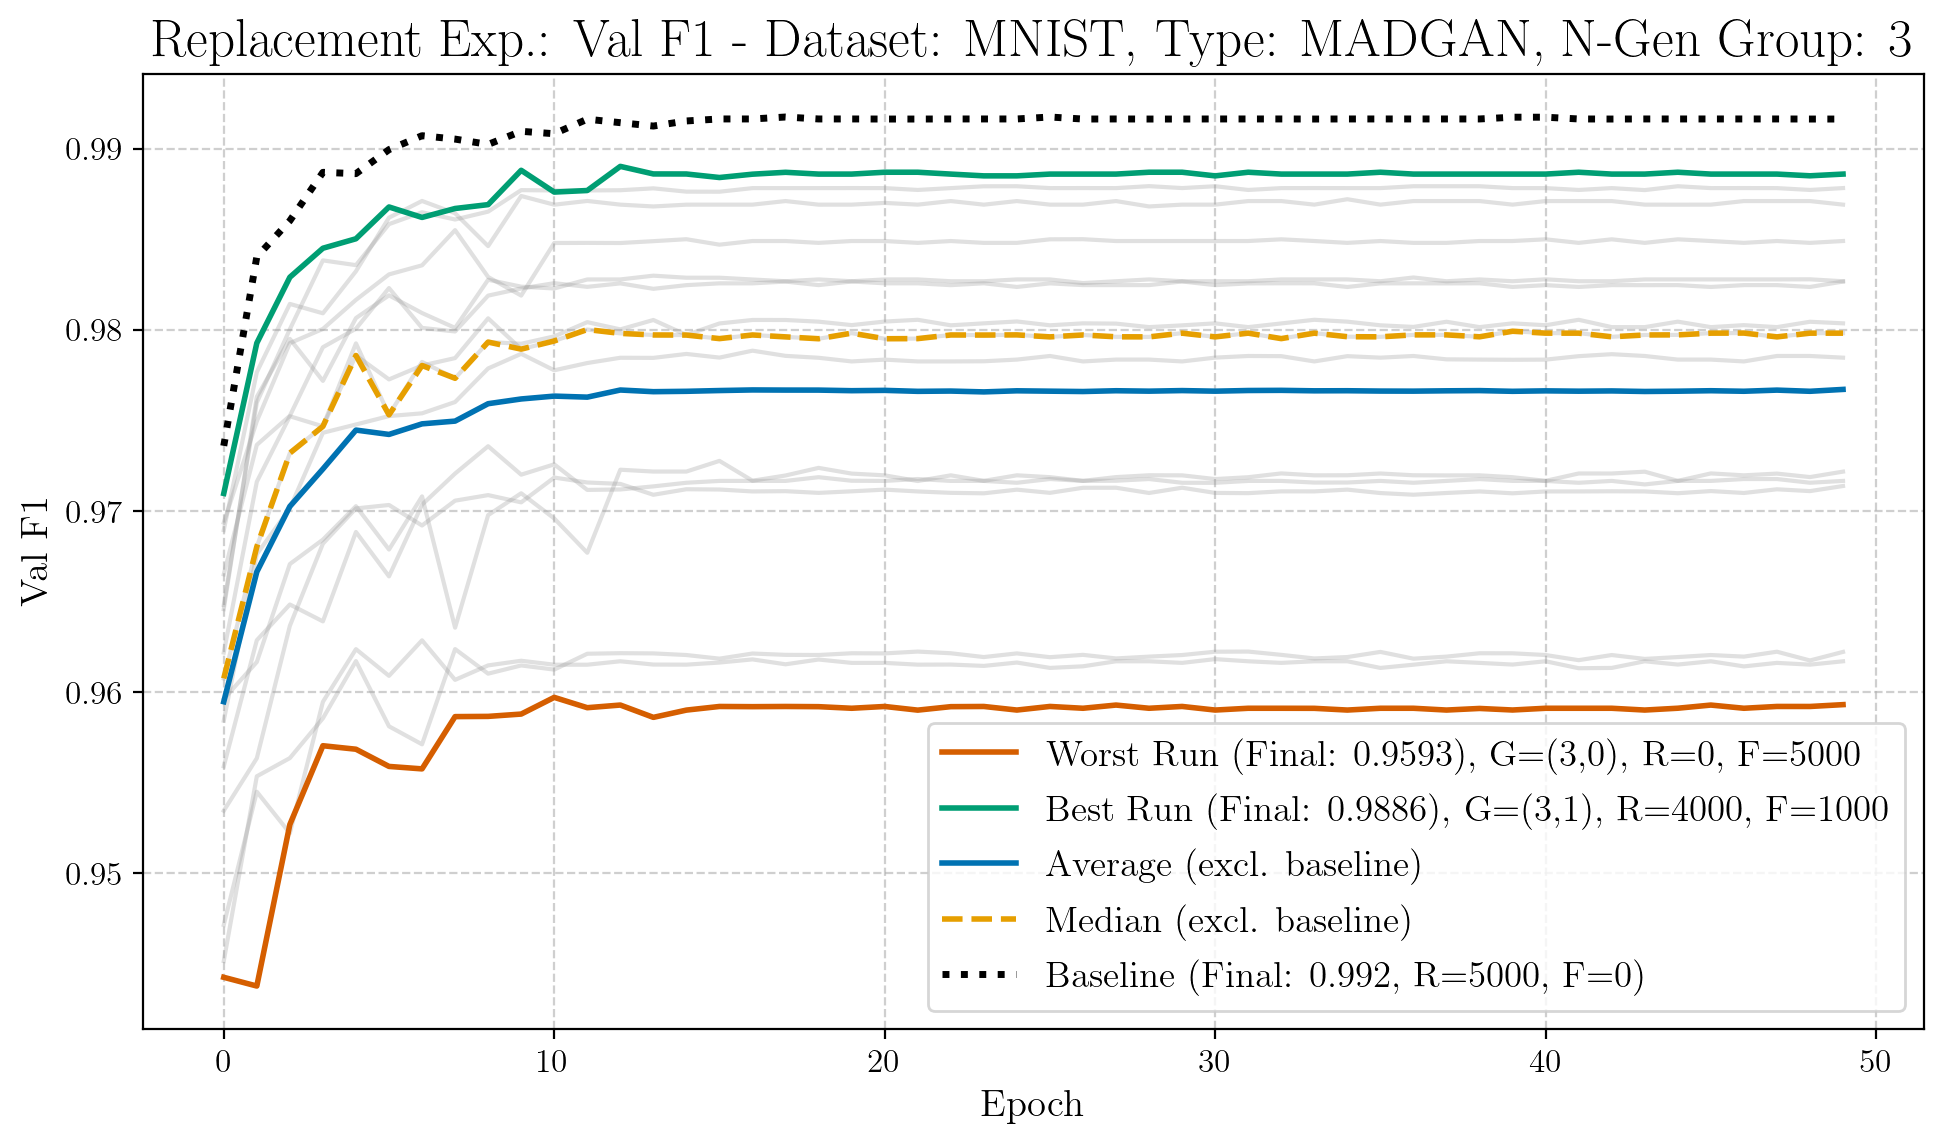
\includegraphics[width=.85\textwidth]{abb/strat_classifier_performance/MNIST_STRATIFIED_CLASSIFIERS_MADGAN_NEW/replacement_experiments/val_f1_score_MADGAN_MNIST_n_gen_3_all.png}
	\label{fig:app_strat_class_performance_replacement_exp._val_f1_score_3}
\end{figure}
\begin{table}[H]
	\vspace{-1.5em}
	\centering
	\begin{tabular}{|c|c|c|c|}
		\hline
		Run Type & Experiment & Val F1 \\ \hline
		best & \(G_{3, 1}\), R:4000, F:1000 & $0.9886$\\ \hline
		worst & \(G_{3, 0}\), R:0, F:5000 & $0.9593$\\ \hline
		median & G (K=3) & $0.9798$\\ \hline
		average & G (K=3) & $0.9767$
		\\ \hline
	\end{tabular}
\end{table}
% End LaTeX Table for Replacement Experiment:
\newpage
% LaTeX Metrics Table for Expansion Experiment: - Metric: val_f1_score - Target Gen Group: 5
\noindent\textbf{Expansion Experiment: K=5}
\begin{figure}[htbp]
	\centering
	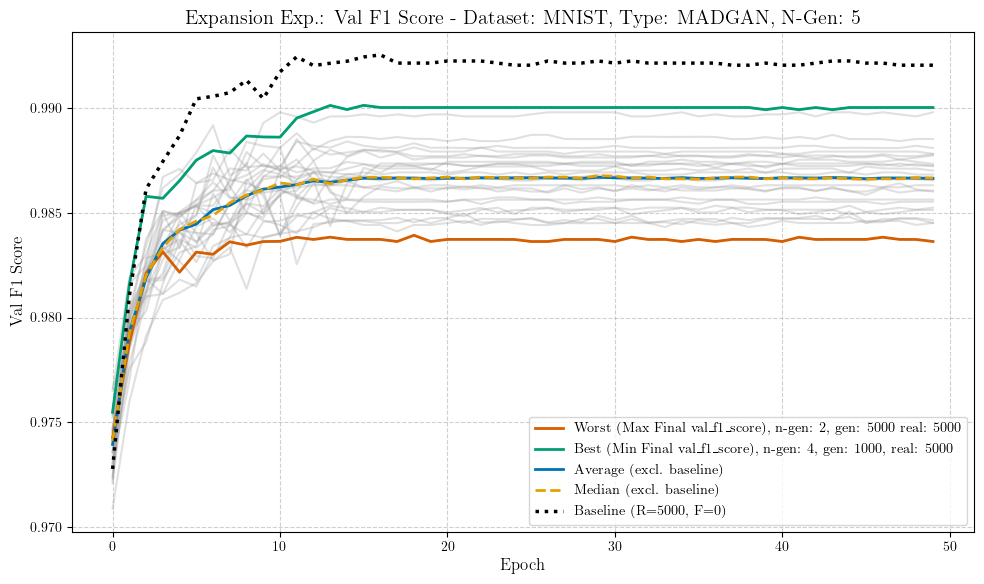
\includegraphics[width=.85\textwidth]{abb/strat_classifier_performance/MNIST_STRATIFIED_CLASSIFIERS_MADGAN_NEW/expansion_experiments/val_f1_score_MADGAN_MNIST_n_gen_5_all.png}
	\label{fig:app_strat_class_performance_expansion_exp._val_f1_score_5}
\end{figure}
\begin{table}[H]
	\vspace{-1em}
	\centering
	\begin{tabular}{|c|c|c|c|}
		\hline
		Run Type & Experiment & Val F1 \\ \hline
		best & \(G_{5, 4}\), R:5000, F:1000 & $0.9900$\\ \hline
		worst & \(G_{5, 2}\), R:5000, F:5000 & $0.9836$\\ \hline
		median & G (K=5) & $0.9867$\\ \hline
		average & G (K=5) & $0.9866$
		\\ \hline
	\end{tabular}
\end{table}
% End LaTeX Table for Expansion Experiment:
% LaTeX Metrics Table for Replacement Experiment: - Metric: val_f1_score - Target Gen Group: 5
\noindent\textbf{Replacement Experiment: K=5}
\begin{figure}[htbp]
	\centering
	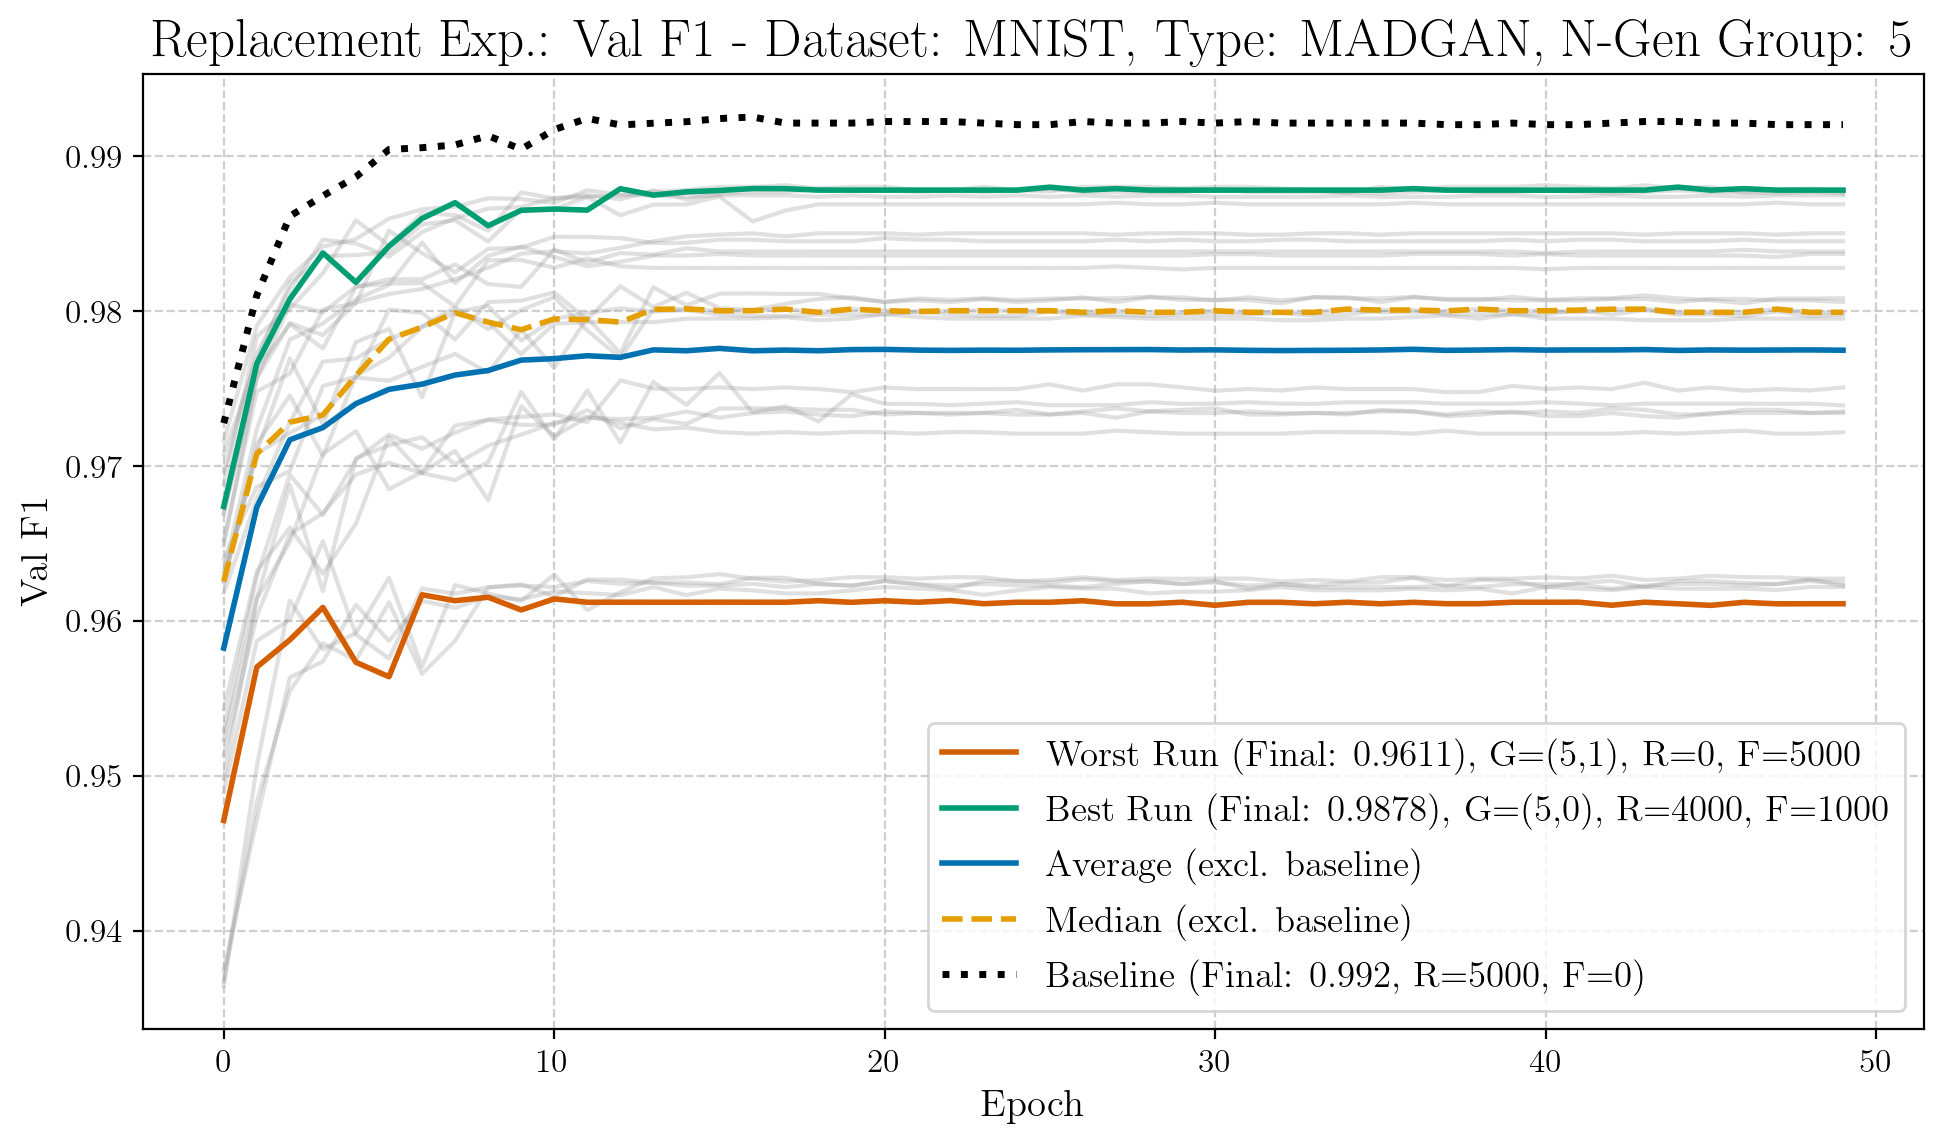
\includegraphics[width=.85\textwidth]{abb/strat_classifier_performance/MNIST_STRATIFIED_CLASSIFIERS_MADGAN_NEW/replacement_experiments/val_f1_score_MADGAN_MNIST_n_gen_5_all.png}
	\label{fig:app_strat_class_performance_replacement_exp._val_f1_score_5}
\end{figure}
\begin{table}[H]
	\vspace{-1em}
	\centering
	\begin{tabular}{|c|c|c|c|}
		\hline
		Run Type & Experiment & Val F1 \\ \hline
		best & \(G_{5, 0}\), R:4000, F:1000 & $0.9878$\\ \hline
		worst & \(G_{5, 1}\), R:0, F:5000 & $0.9611$\\ \hline
		median & G (K=5) & $0.9799$\\ \hline
		average & G (K=5) & $0.9775$
		\\ \hline
	\end{tabular}
\end{table}
% End LaTeX Table for Replacement Experiment:
\newpage
% LaTeX Metrics Table for Expansion Experiment: - Metric: val_f1_score - Target Gen Group: 7
\noindent\textbf{Expansion Experiment: K=7}
\begin{figure}[htbp]
	\centering
	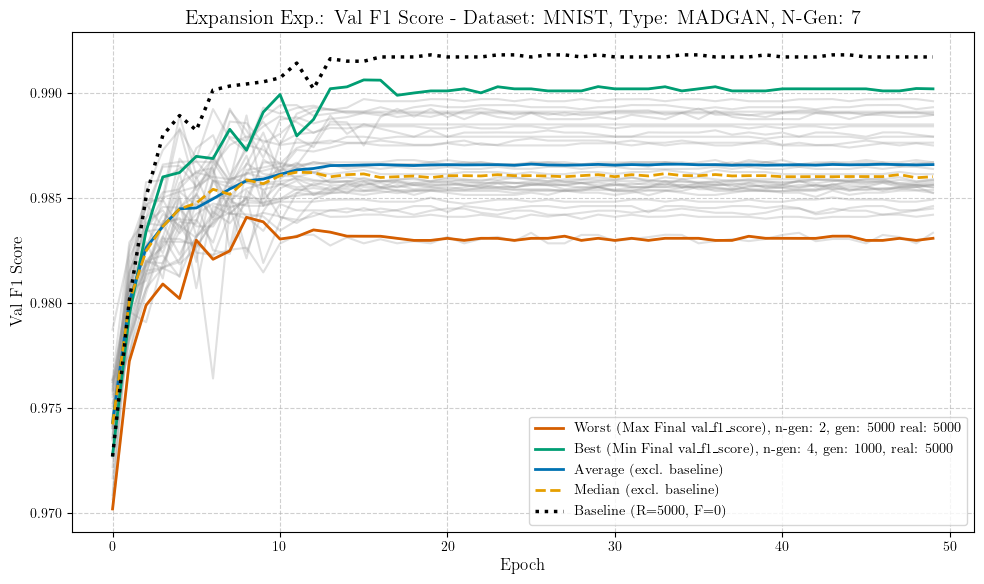
\includegraphics[width=.85\textwidth]{abb/strat_classifier_performance/MNIST_STRATIFIED_CLASSIFIERS_MADGAN_NEW/expansion_experiments/val_f1_score_MADGAN_MNIST_n_gen_7_all.png}
	\label{fig:app_strat_class_performance_expansion_exp._val_f1_score_7}
\end{figure}
\begin{table}[H]
	\vspace{-1em}
	\centering
	\begin{tabular}{|c|c|c|c|}
		\hline
		Run Type & Experiment & Val F1 \\ \hline
		best & \(G_{7, 4}\), R:5000, F:1000 & $0.9902$\\ \hline
		worst & \(G_{7, 2}\), R:5000, F:5000 & $0.9831$\\ \hline
		median & G (K=7) & $0.9860$\\ \hline
		average & G (K=7) & $0.9866$
		\\ \hline
	\end{tabular}
\end{table}
% End LaTeX Table for Expansion Experiment:
% LaTeX Metrics Table for Replacement Experiment: - Metric: val_f1_score - Target Gen Group: 7
\noindent\textbf{Replacement Experiment: K=7}
\begin{figure}[htbp]
	\centering
	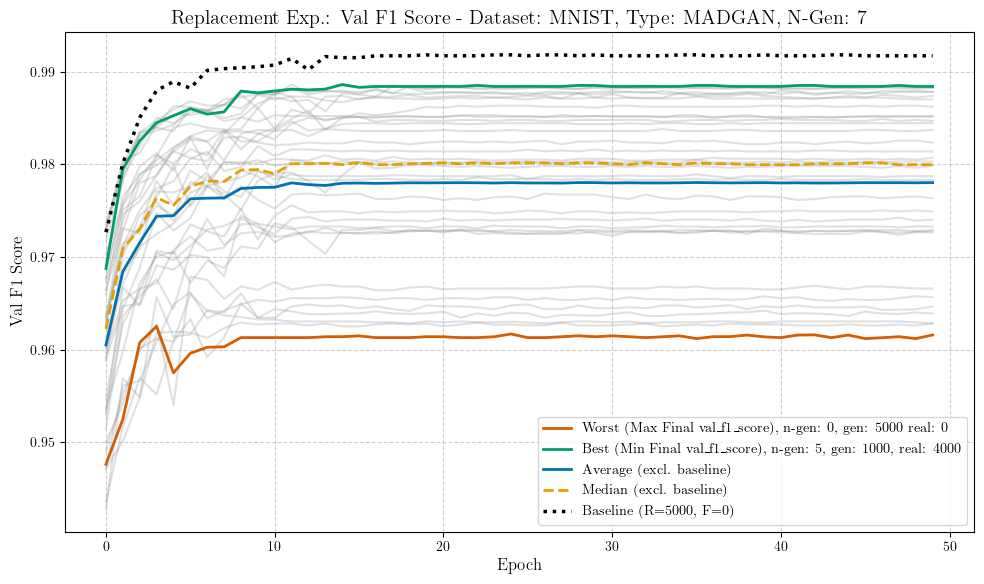
\includegraphics[width=.85\textwidth]{abb/strat_classifier_performance/MNIST_STRATIFIED_CLASSIFIERS_MADGAN_NEW/replacement_experiments/val_f1_score_MADGAN_MNIST_n_gen_7_all.png}
	\label{fig:app_strat_class_performance_replacement_exp._val_f1_score_7}
\end{figure}
\begin{table}[H]
	\vspace{-1em}
	\centering
	\begin{tabular}{|c|c|c|c|}
		\hline
		Run Type & Experiment & Val F1 \\ \hline
		best & \(G_{7, 5}\), R:4000, F:1000 & $0.9884$\\ \hline
		worst & \(G_{7, 0}\), R:0, F:5000 & $0.9616$\\ \hline
		median & G (K=7) & $0.9800$\\ \hline
		average & G (K=7) & $0.9780$
		\\ \hline
	\end{tabular}
\end{table}
% End LaTeX Table for Replacement Experiment:
\newpage
% LaTeX Metrics Table for Expansion Experiment: - Metric: val_f1_score - Target Gen Group: 10
\noindent\textbf{Expansion Experiment: K=10}
\begin{figure}[htbp]
	\centering
	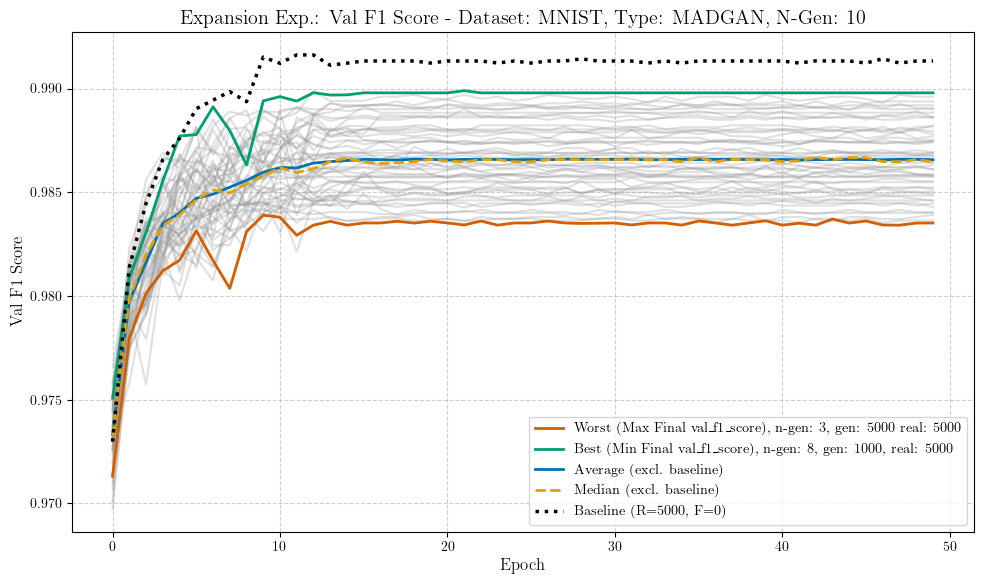
\includegraphics[width=.85\textwidth]{abb/strat_classifier_performance/MNIST_STRATIFIED_CLASSIFIERS_MADGAN_NEW/expansion_experiments/val_f1_score_MADGAN_MNIST_n_gen_10_all.png}
	\label{fig:app_strat_class_performance_expansion_exp._val_f1_score_10}
\end{figure}
\begin{table}[H]
	\vspace{-1em}
	\centering
	\begin{tabular}{|c|c|c|c|}
		\hline
		Run Type & Experiment & Val F1 \\ \hline
		best & \(G_{10, 8}\), R:5000, F:1000 & $0.9898$\\ \hline
		worst & \(G_{10, 3}\), R:5000, F:5000 & $0.9835$\\ \hline
		median & G (K=10) & $0.9865$\\ \hline
		average & G (K=10) & $0.9866$
		\\ \hline
	\end{tabular}
\end{table}
% End LaTeX Table for Expansion Experiment:
% LaTeX Metrics Table for Replacement Experiment: - Metric: val_f1_score - Target Gen Group: 10
\noindent\textbf{Replacement Experiment: K=10}
\begin{figure}[htbp]
	\centering
	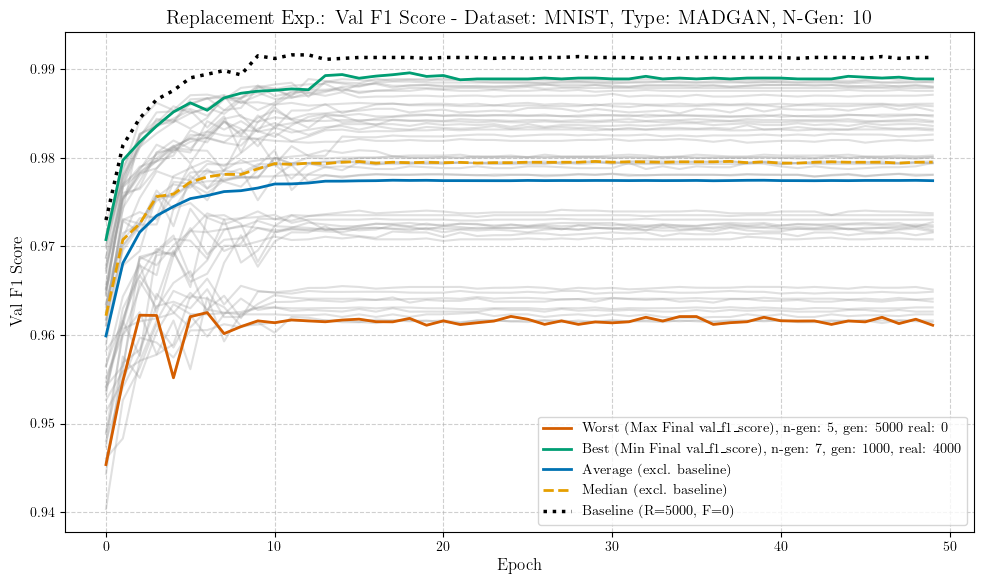
\includegraphics[width=.85\textwidth]{abb/strat_classifier_performance/MNIST_STRATIFIED_CLASSIFIERS_MADGAN_NEW/replacement_experiments/val_f1_score_MADGAN_MNIST_n_gen_10_all.png}
	\label{fig:app_strat_class_performance_replacement_exp._val_f1_score_10}
\end{figure}
\begin{table}[H]
	\vspace{-1em}
	\centering
	\begin{tabular}{|c|c|c|c|}
		\hline
		Run Type & Experiment & Val F1 \\ \hline
		best & \(G_{10, 7}\), R:4000, F:1000 & $0.9889$\\ \hline
		worst & \(G_{10, 5}\), R:0, F:5000 & $0.9611$\\ \hline
		median & G (K=10) & $0.9795$\\ \hline
		average & G (K=10) & $0.9774$
		\\ \hline
	\end{tabular}
\end{table}
% End LaTeX Table for Replacement Experiment:
\newpage
\subsubsection{Dataset: MNIST, Architecture: cMADGAN}
% LaTeX Metrics Table for Expansion Experiment: - Metric: val_f1_score - Target Gen Group: 3
\noindent\textbf{Expansion Experiment: K=3}
\begin{figure}[htbp]
	\centering
	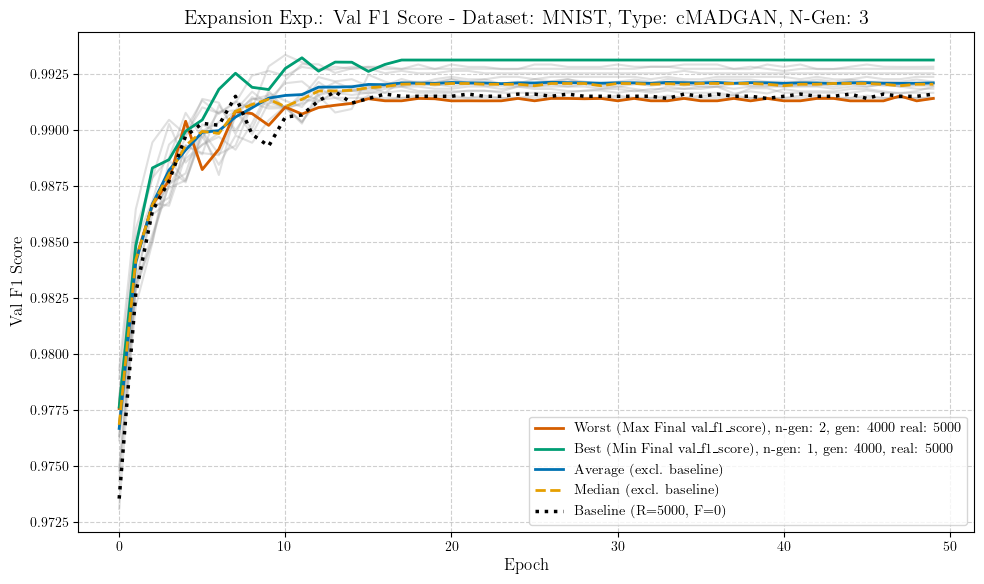
\includegraphics[width=.85\textwidth]{abb/strat_classifier_performance/MNIST_STRATIFIED_CLASSIFIERS_cMADGAN_NEW/expansion_experiments/val_f1_score_cMADGAN_MNIST_n_gen_3_all.png}
	\label{fig:app_strat_class_performance_expansion_exp._val_f1_score_3}
\end{figure}
\begin{table}[H]
	\vspace{-1em}
	\centering
	\begin{tabular}{|c|c|c|c|}
		\hline
		Run Type & Experiment & Val F1 \\ \hline
		best & \(G_{3, 1}\), R:5000, F:4000 & $0.9931$\\ \hline
		worst & \(G_{3, 2}\), R:5000, F:4000 & $0.9914$\\ \hline
		median & G (K=3) & $0.9920$\\ \hline
		average & G (K=3) & $0.9921$
		\\ \hline
	\end{tabular}
\end{table}
% End LaTeX Table for Expansion Experiment:
% LaTeX Metrics Table for Replacement Experiment: - Metric: val_f1_score - Target Gen Group: 3
\noindent\textbf{Replacement Experiment: K=3}
\begin{figure}[htbp]
	\centering
	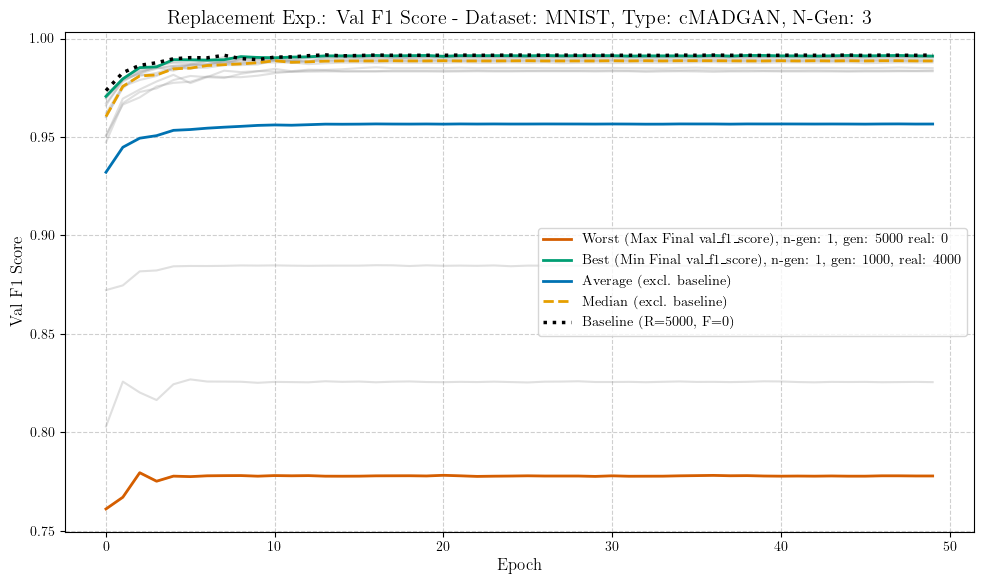
\includegraphics[width=.85\textwidth]{abb/strat_classifier_performance/MNIST_STRATIFIED_CLASSIFIERS_cMADGAN_NEW/replacement_experiments/val_f1_score_cMADGAN_MNIST_n_gen_3_all.png}
	\label{fig:app_strat_class_performance_replacement_exp._val_f1_score_3}
\end{figure}
\begin{table}[H]
	\vspace{-1em}
	\centering
	\begin{tabular}{|c|c|c|c|}
		\hline
		Run Type & Experiment & Val F1 \\ \hline
		best & \(G_{3, 1}\), R:4000, F:1000 & $0.9911$\\ \hline
		worst & \(G_{3, 1}\), R:0, F:5000 & $0.7778$\\ \hline
		median & G (K=3) & $0.9886$\\ \hline
		average & G (K=3) & $0.9566$
		\\ \hline
	\end{tabular}
\end{table}
% End LaTeX Table for Replacement Experiment:
\newpage
% LaTeX Metrics Table for Expansion Experiment: - Metric: val_f1_score - Target Gen Group: 5
\noindent\textbf{Expansion Experiment: K=5}
\begin{figure}[htbp]
	\centering
	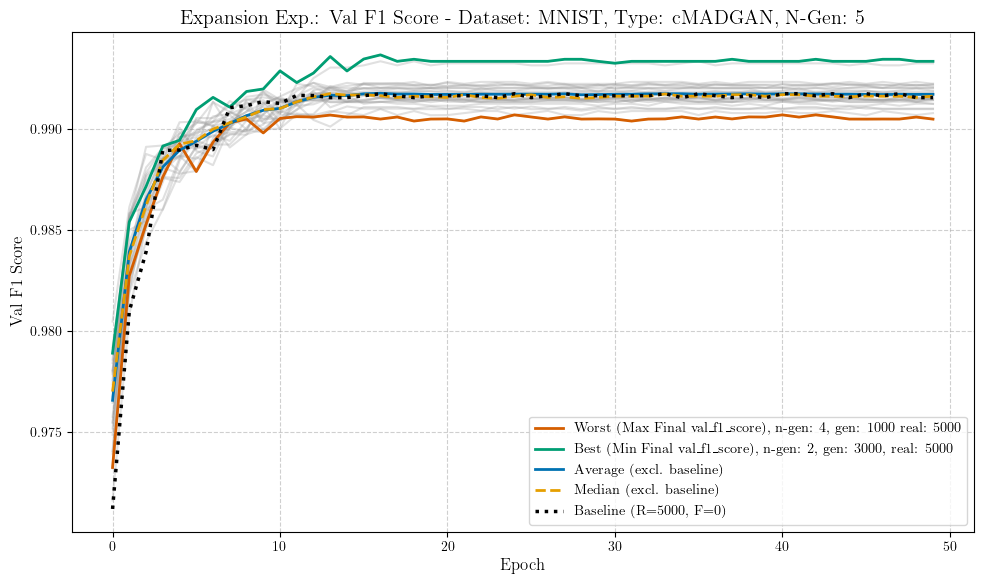
\includegraphics[width=.85\textwidth]{abb/strat_classifier_performance/MNIST_STRATIFIED_CLASSIFIERS_cMADGAN_NEW/expansion_experiments/val_f1_score_cMADGAN_MNIST_n_gen_5_all.png}
	\label{fig:app_strat_class_performance_expansion_exp._val_f1_score_5}
\end{figure}
\begin{table}[H]
	\vspace{-1em}
	\centering
	\begin{tabular}{|c|c|c|c|}
		\hline
		Run Type & Experiment & Val F1 \\ \hline
		best & \(G_{5, 2}\), R:5000, F:3000 & $0.9933$\\ \hline
		worst & \(G_{5, 4}\), R:5000, F:1000 & $0.9905$\\ \hline
		median & G (K=5) & $0.9916$\\ \hline
		average & G (K=5) & $0.9917$
		\\ \hline
	\end{tabular}
\end{table}
% End LaTeX Table for Expansion Experiment:
% LaTeX Metrics Table for Replacement Experiment: - Metric: val_f1_score - Target Gen Group: 5
\noindent\textbf{Replacement Experiment: K=5}
\begin{figure}[htbp]
	\centering
	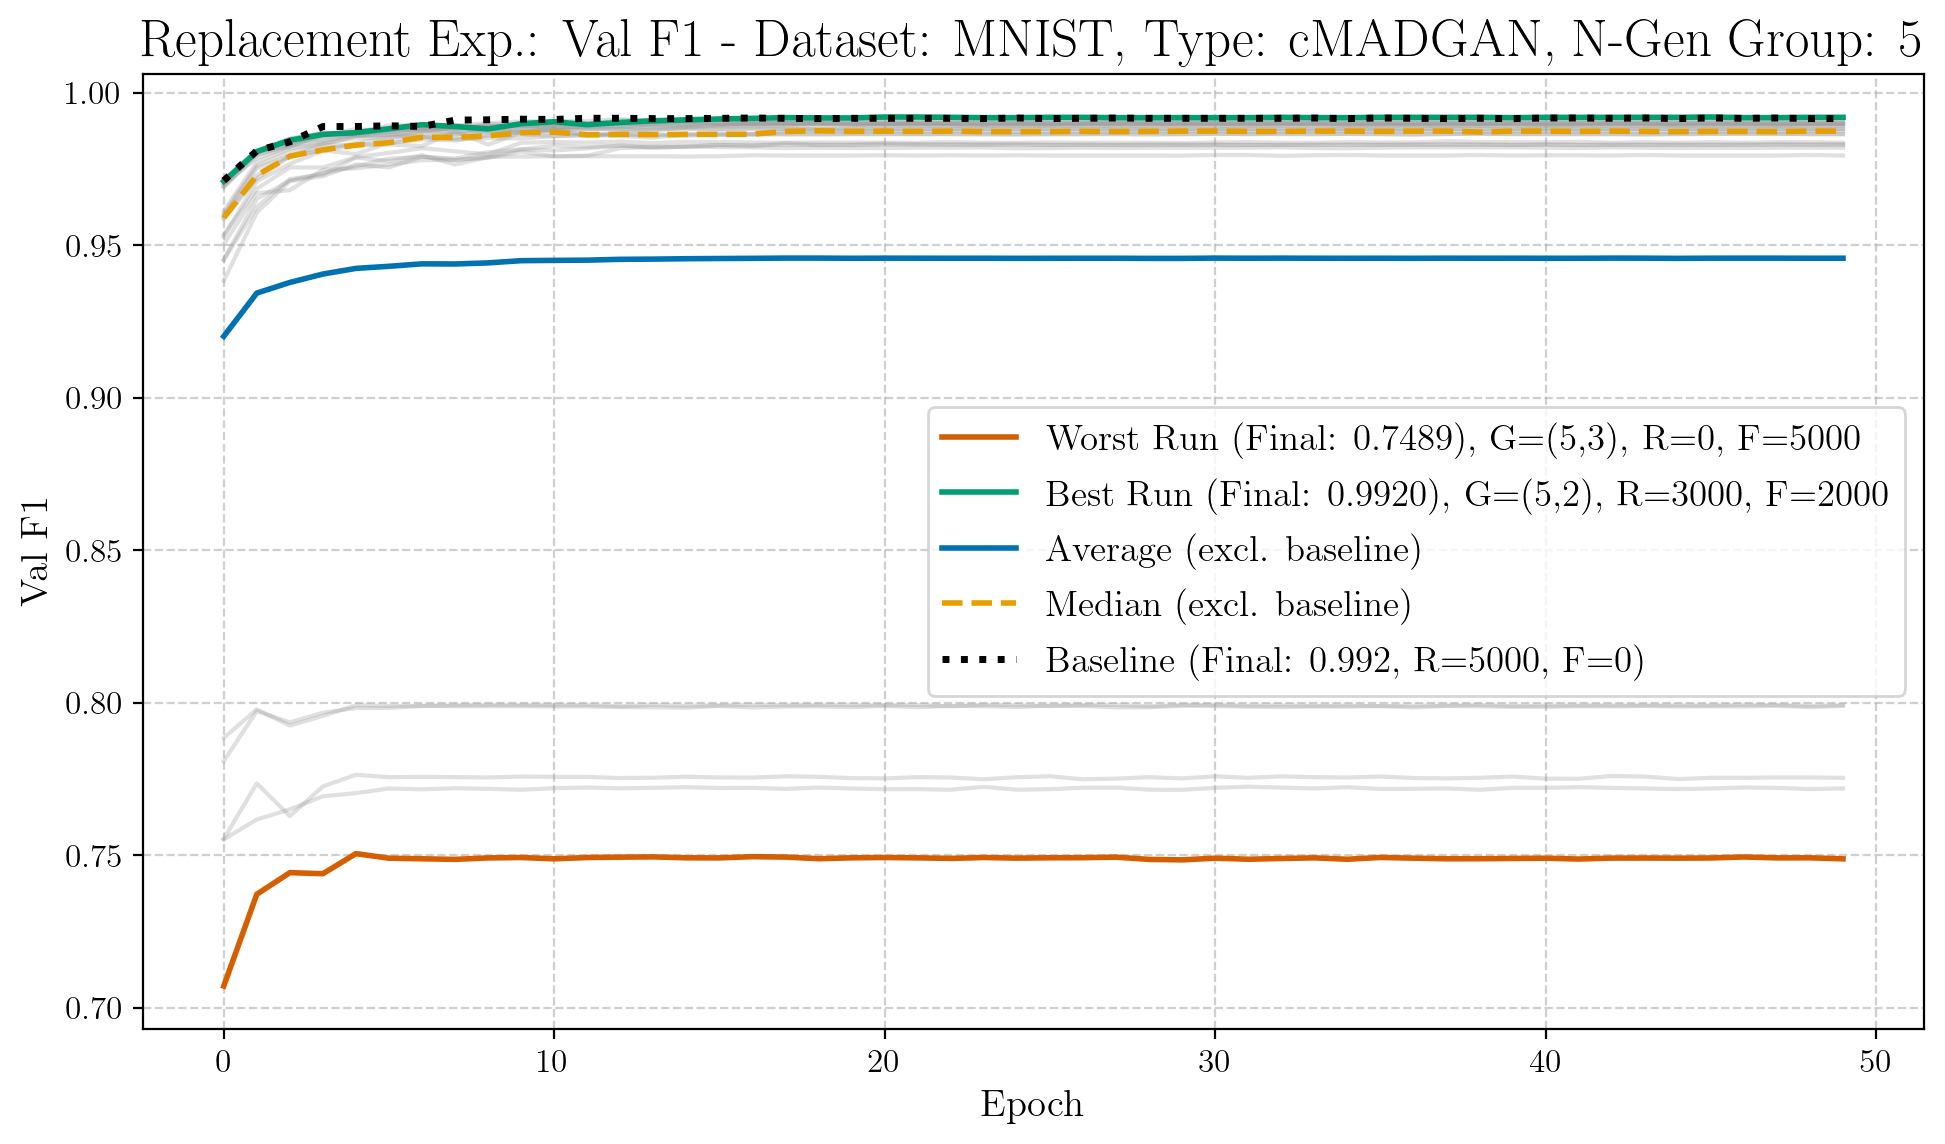
\includegraphics[width=.85\textwidth]{abb/strat_classifier_performance/MNIST_STRATIFIED_CLASSIFIERS_cMADGAN_NEW/replacement_experiments/val_f1_score_cMADGAN_MNIST_n_gen_5_all.png}
	\label{fig:app_strat_class_performance_replacement_exp._val_f1_score_5}
\end{figure}
\begin{table}[H]
	\vspace{-1em}
	\centering
	\begin{tabular}{|c|c|c|c|}
		\hline
		Run Type & Experiment & Val F1 \\ \hline
		best & \(G_{5, 2}\), R:3000, F:2000 & $0.9920$\\ \hline
		worst & \(G_{5, 3}\), R:0, F:5000 & $0.7489$\\ \hline
		median & G (K=5) & $0.9874$\\ \hline
		average & G (K=5) & $0.9458$
		\\ \hline
	\end{tabular}
\end{table}
% End LaTeX Table for Replacement Experiment:
\newpage
% LaTeX Metrics Table for Expansion Experiment: - Metric: val_f1_score - Target Gen Group: 7
\noindent\textbf{Expansion Experiment: K=7}
\begin{figure}[htbp]
	\centering
	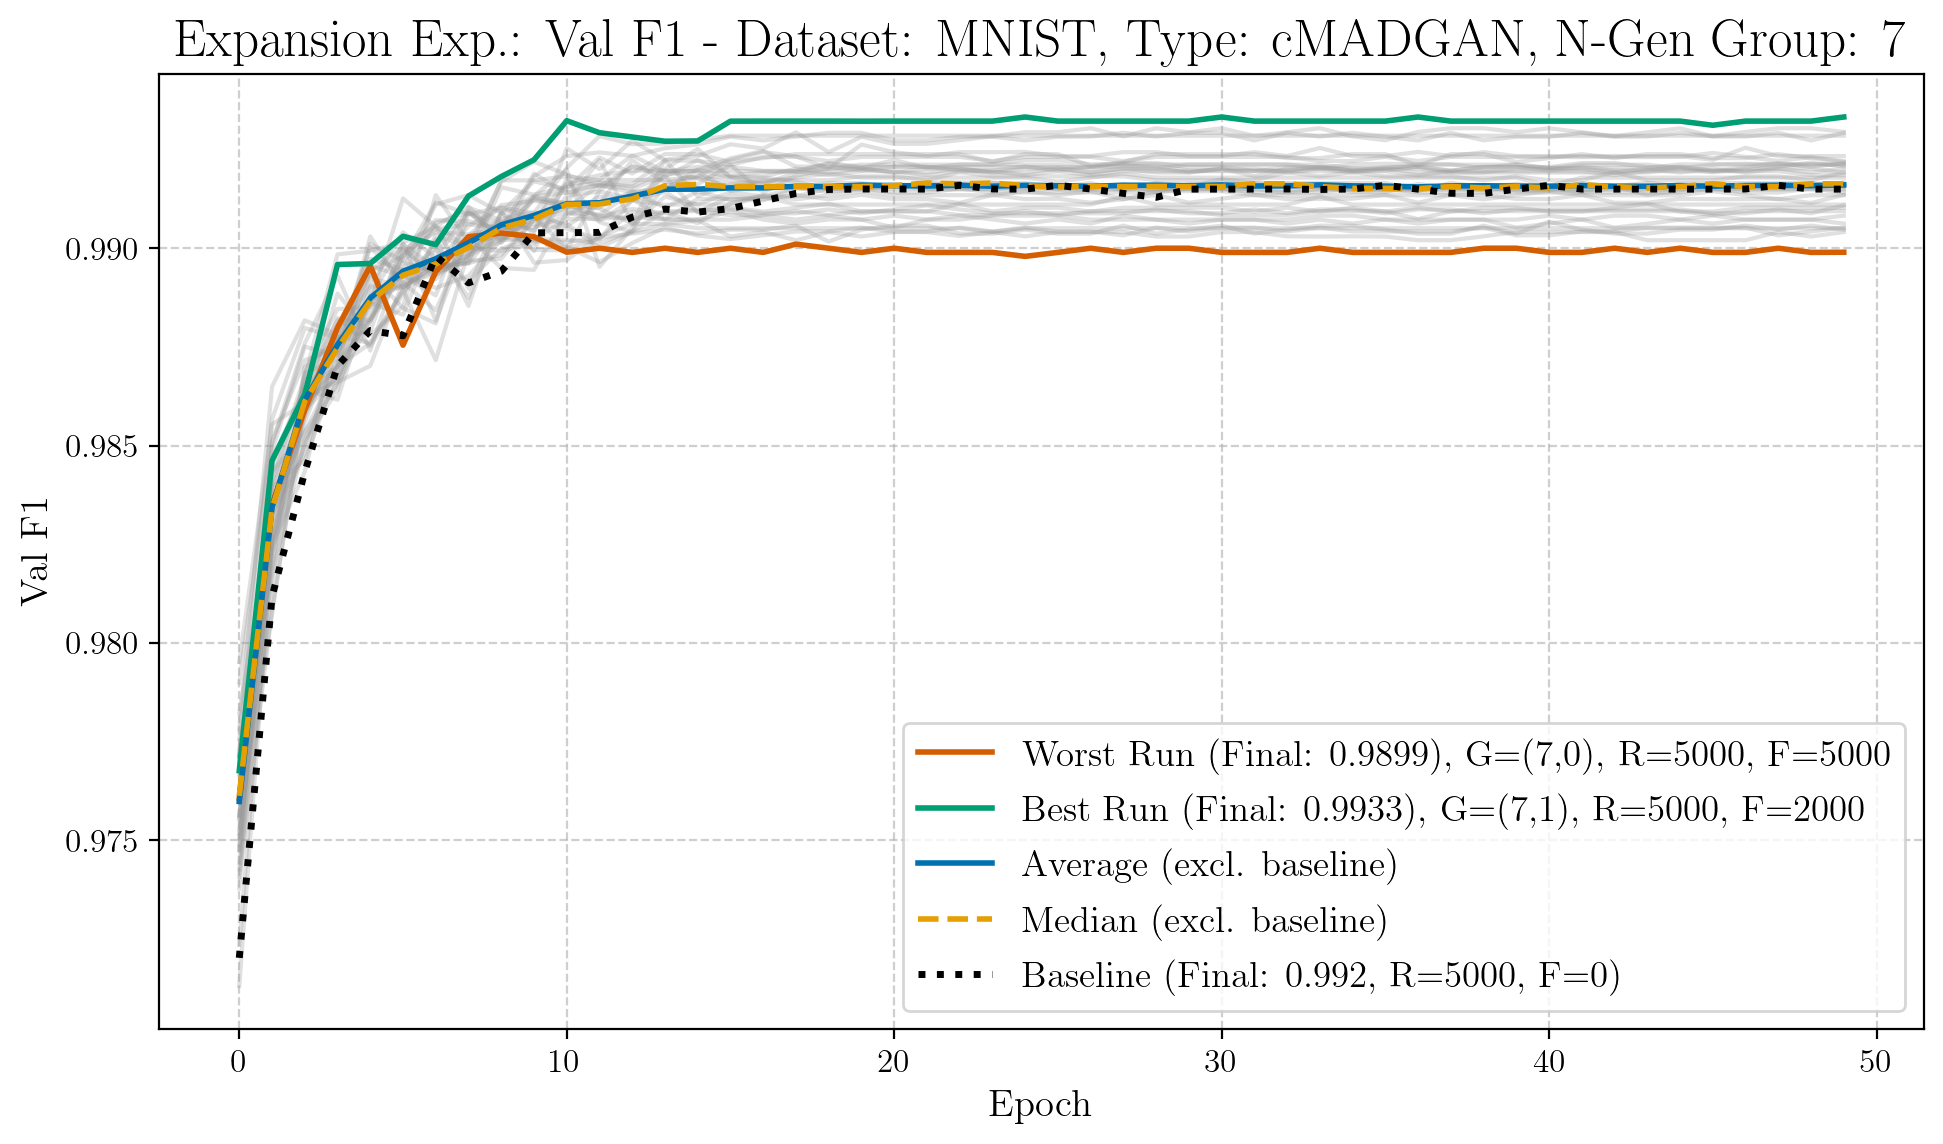
\includegraphics[width=.85\textwidth]{abb/strat_classifier_performance/MNIST_STRATIFIED_CLASSIFIERS_cMADGAN_NEW/expansion_experiments/val_f1_score_cMADGAN_MNIST_n_gen_7_all.png}
	\label{fig:app_strat_class_performance_expansion_exp._val_f1_score_7}
\end{figure}
\begin{table}[H]
	\vspace{-1em}
	\centering
	\begin{tabular}{|c|c|c|c|}
		\hline
		Run Type & Experiment & Val F1 \\ \hline
		best & \(G_{7, 1}\), R:5000, F:2000 & $0.9933$\\ \hline
		worst & \(G_{7, 0}\), R:5000, F:5000 & $0.9899$\\ \hline
		median & G (K=7) & $0.9916$\\ \hline
		average & G (K=7) & $0.9916$
		\\ \hline
	\end{tabular}
\end{table}
% End LaTeX Table for Expansion Experiment:
% LaTeX Metrics Table for Replacement Experiment: - Metric: val_f1_score - Target Gen Group: 7
\noindent\textbf{Replacement Experiment: K=7}
\begin{figure}[htbp]
	\centering
	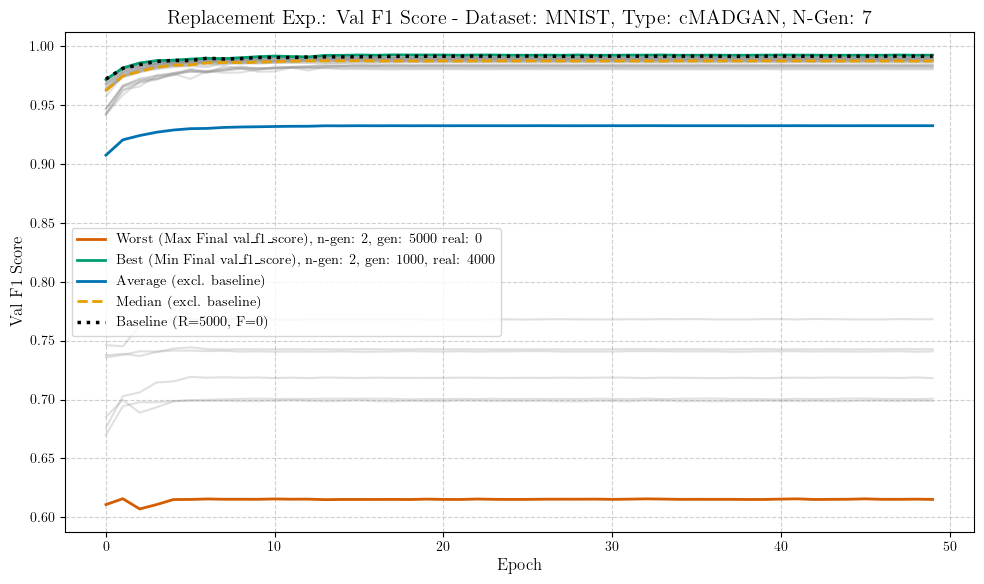
\includegraphics[width=.85\textwidth]{abb/strat_classifier_performance/MNIST_STRATIFIED_CLASSIFIERS_cMADGAN_NEW/replacement_experiments/val_f1_score_cMADGAN_MNIST_n_gen_7_all.png}
	\label{fig:app_strat_class_performance_replacement_exp._val_f1_score_7}
\end{figure}
\begin{table}[H]
	\vspace{-1em}
	\centering
	\begin{tabular}{|c|c|c|c|}
		\hline
		Run Type & Experiment & Val F1 \\ \hline
		best & \(G_{7, 2}\), R:4000, F:1000 & $0.9924$\\ \hline
		worst & \(G_{7, 2}\), R:0, F:5000 & $0.6152$\\ \hline
		median & G (K=7) & $0.9874$\\ \hline
		average & G (K=7) & $0.9325$
		\\ \hline
	\end{tabular}
\end{table}
% End LaTeX Table for Replacement Experiment:
\newpage
% LaTeX Metrics Table for Expansion Experiment: - Metric: val_f1_score - Target Gen Group: 10
\noindent\textbf{Expansion Experiment: K=10}
\begin{figure}[htbp]
	\centering
	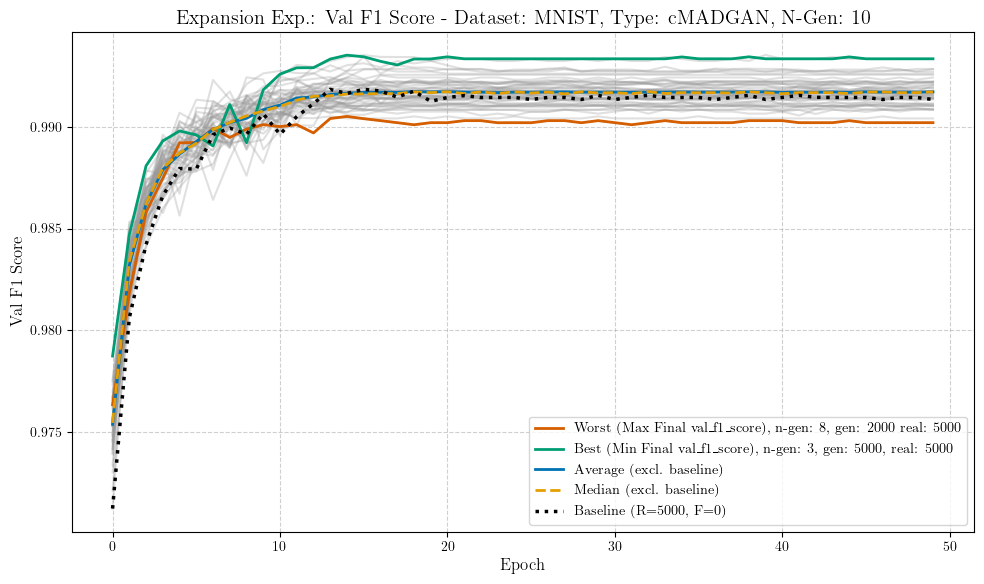
\includegraphics[width=.85\textwidth]{abb/strat_classifier_performance/MNIST_STRATIFIED_CLASSIFIERS_cMADGAN_NEW/expansion_experiments/val_f1_score_cMADGAN_MNIST_n_gen_10_all.png}
	\label{fig:app_strat_class_performance_expansion_exp._val_f1_score_10}
\end{figure}
\begin{table}[H]
	\vspace{-1em}
	\centering
	\begin{tabular}{|c|c|c|c|}
		\hline
		Run Type & Experiment & Val F1 \\ \hline
		best & \(G_{10, 3}\), R:5000, F:5000 & $0.9933$\\ \hline
		worst & \(G_{10, 8}\), R:5000, F:2000 & $0.9902$\\ \hline
		median & G (K=10) & $0.9917$\\ \hline
		average & G (K=10) & $0.9917$
		\\ \hline
	\end{tabular}
\end{table}
% End LaTeX Table for Expansion Experiment:
% LaTeX Metrics Table for Replacement Experiment: - Metric: val_f1_score - Target Gen Group: 10
\noindent\textbf{Replacement Experiment: K=10}
\begin{figure}[htbp]
	\centering
	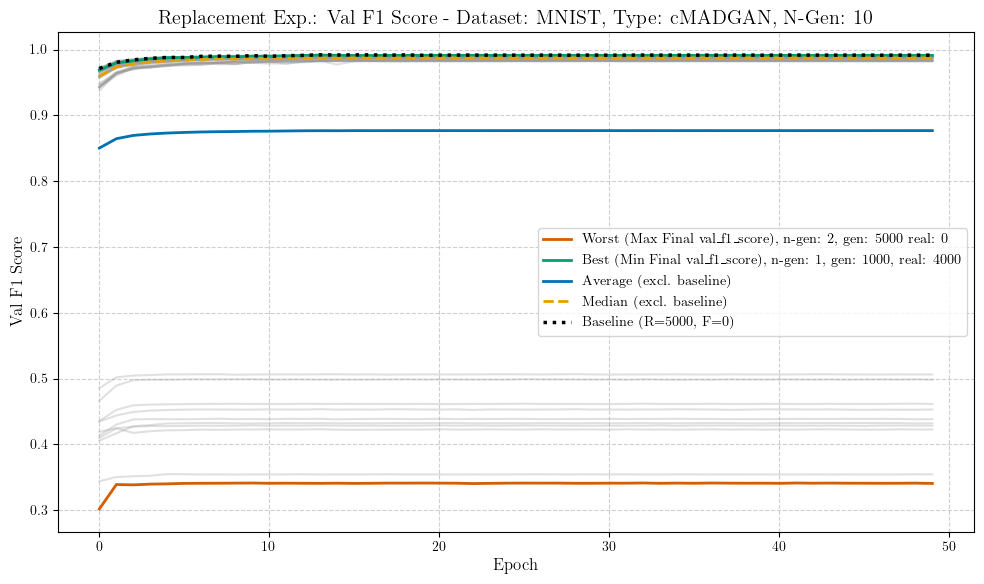
\includegraphics[width=.85\textwidth]{abb/strat_classifier_performance/MNIST_STRATIFIED_CLASSIFIERS_cMADGAN_NEW/replacement_experiments/val_f1_score_cMADGAN_MNIST_n_gen_10_all.png}
	\label{fig:app_strat_class_performance_replacement_exp._val_f1_score_10}
\end{figure}
\begin{table}[H]
	\vspace{-1em}
	\centering
	\begin{tabular}{|c|c|c|c|}
		\hline
		Run Type & Experiment & Val F1 \\ \hline
		best & \(G_{10, 1}\), R:4000, F:1000 & $0.9911$\\ \hline
		worst & \(G_{10, 2}\), R:0, F:5000 & $0.3407$\\ \hline
		median & G (K=10) & $0.9872$\\ \hline
		average & G (K=10) & $0.8768$
		\\ \hline
	\end{tabular}
\end{table}
% End LaTeX Table for Replacement Experiment:
\newpage
\subsubsection{Dataset: FASHION, Architecture: MADGAN}
% LaTeX Metrics Table for Expansion Experiment: - Metric: val_f1_score - Target Gen Group: 3
\noindent\textbf{Expansion Experiment: K=3}
\begin{figure}[htbp]
	\centering
	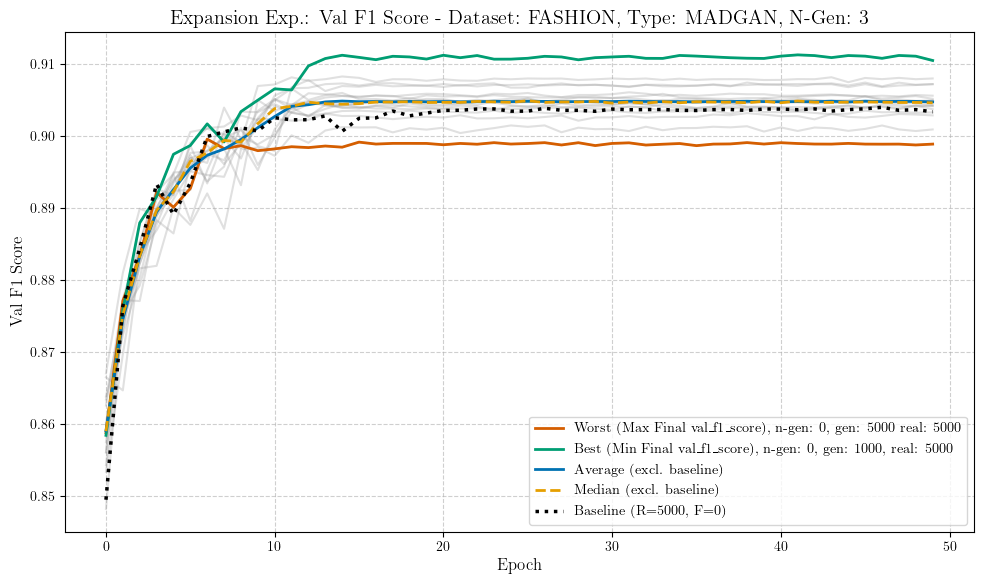
\includegraphics[width=.85\textwidth]{abb/strat_classifier_performance/FASHION_STRATIFIED_CLASSIFIERS_MADGAN_NEW/expansion_experiments/val_f1_score_MADGAN_FASHION_n_gen_3_all.png}
	\label{fig:app_strat_class_performance_expansion_exp._val_f1_score_3}
\end{figure}
\begin{table}[H]
	\vspace{-1em}
	\centering
	\begin{tabular}{|c|c|c|c|}
		\hline
		Run Type & Experiment & Val F1 \\ \hline
		best & \(G_{3, 0}\), R:5000, F:1000 & $0.9105$\\ \hline
		worst & \(G_{3, 0}\), R:5000, F:5000 & $0.8989$\\ \hline
		median & G (K=3) & $0.9046$\\ \hline
		average & G (K=3) & $0.9048$
		\\ \hline
	\end{tabular}
\end{table}
% End LaTeX Table for Expansion Experiment:
% LaTeX Metrics Table for Replacement Experiment: - Metric: val_f1_score - Target Gen Group: 3
\noindent\textbf{Replacement Experiment: K=3}
\begin{figure}[htbp]
	\centering
	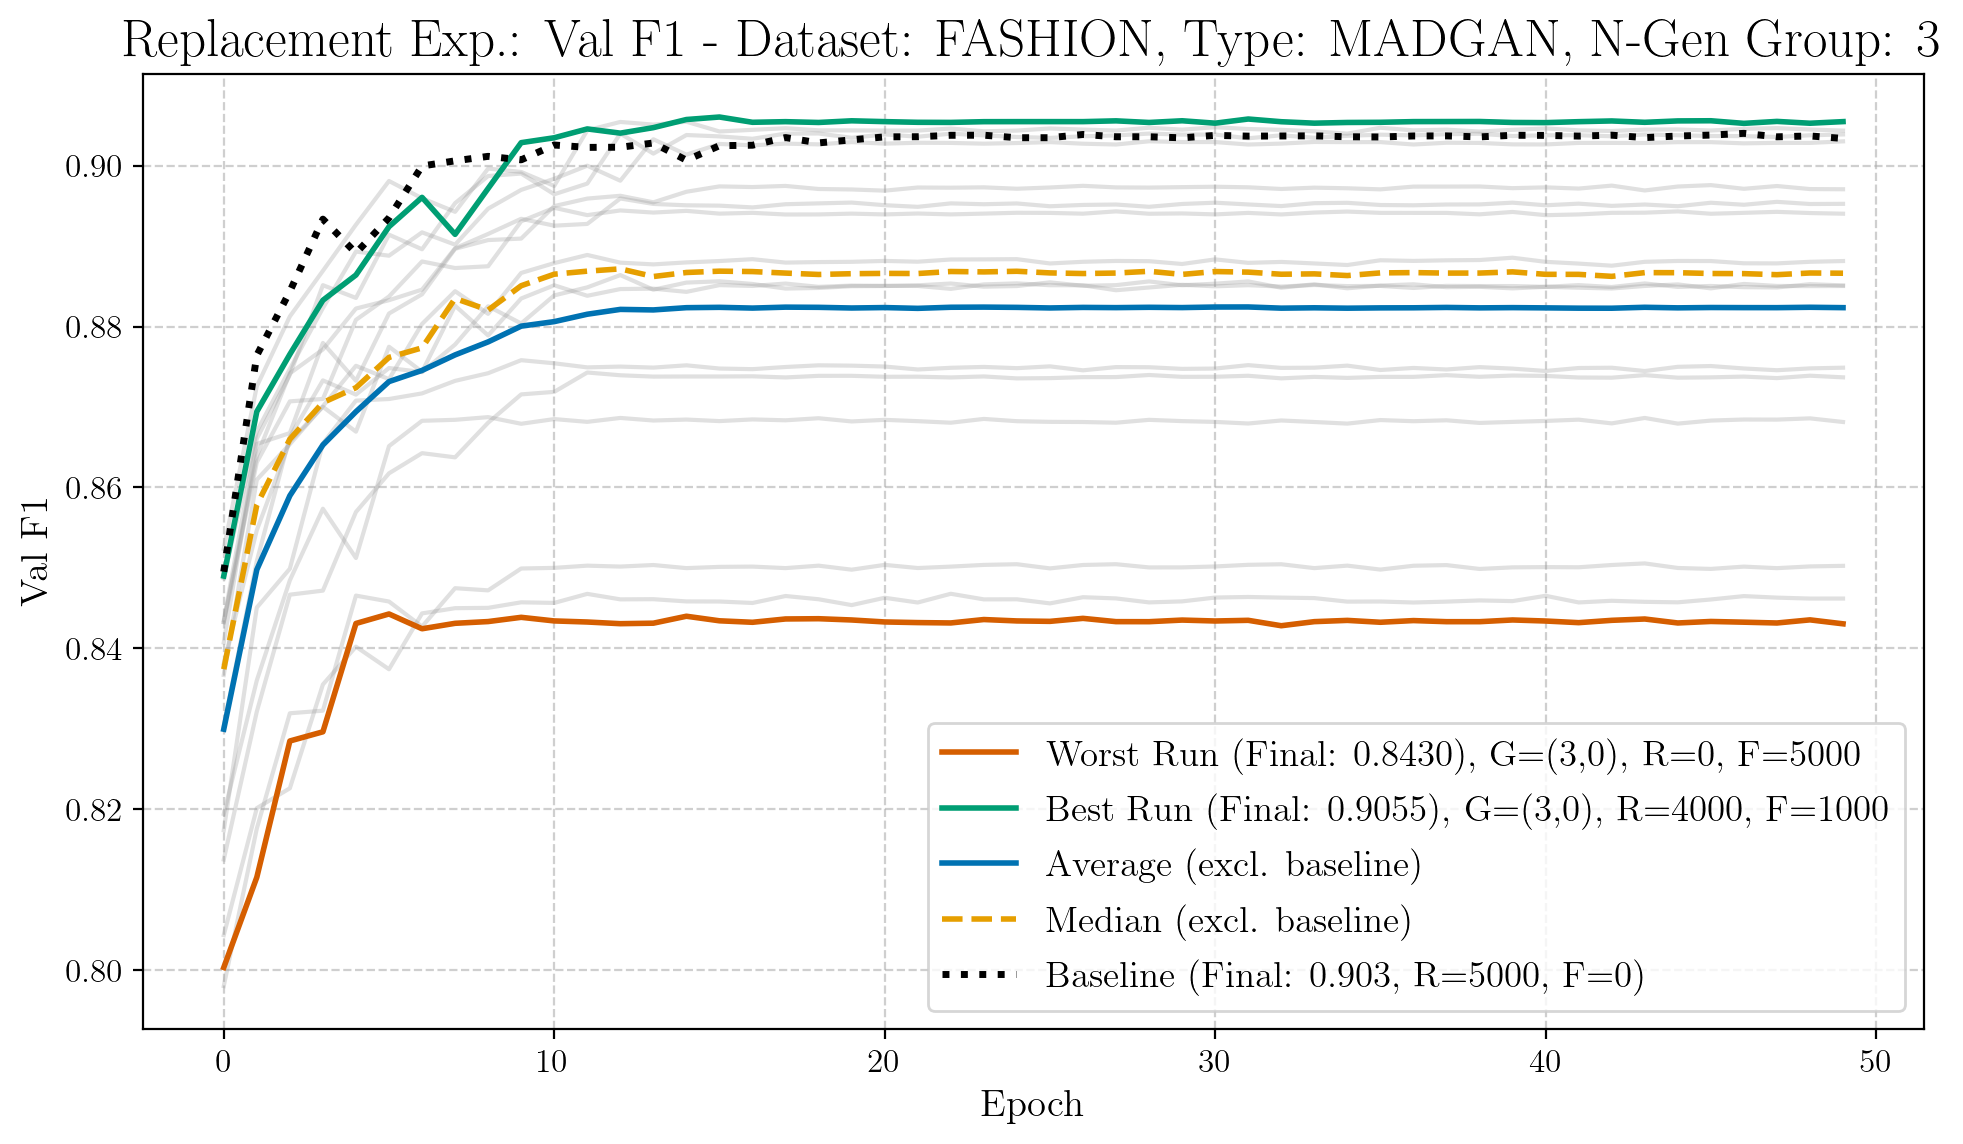
\includegraphics[width=.85\textwidth]{abb/strat_classifier_performance/FASHION_STRATIFIED_CLASSIFIERS_MADGAN_NEW/replacement_experiments/val_f1_score_MADGAN_FASHION_n_gen_3_all.png}
	\label{fig:app_strat_class_performance_replacement_exp._val_f1_score_3}
\end{figure}
\begin{table}[H]
	\vspace{-1em}
	\centering
	\begin{tabular}{|c|c|c|c|}
		\hline
		Run Type & Experiment & Val F1 \\ \hline
		best & \(G_{3, 0}\), R:4000, F:1000 & $0.9055$\\ \hline
		worst & \(G_{3, 0}\), R:0, F:5000 & $0.8430$\\ \hline
		median & G (K=3) & $0.8866$\\ \hline
		average & G (K=3) & $0.8824$
		\\ \hline
	\end{tabular}
\end{table}
% End LaTeX Table for Replacement Experiment:
\newpage
% LaTeX Metrics Table for Expansion Experiment: - Metric: val_f1_score - Target Gen Group: 5
\noindent\textbf{Expansion Experiment: K=5}
\begin{figure}[htbp]
	\centering
	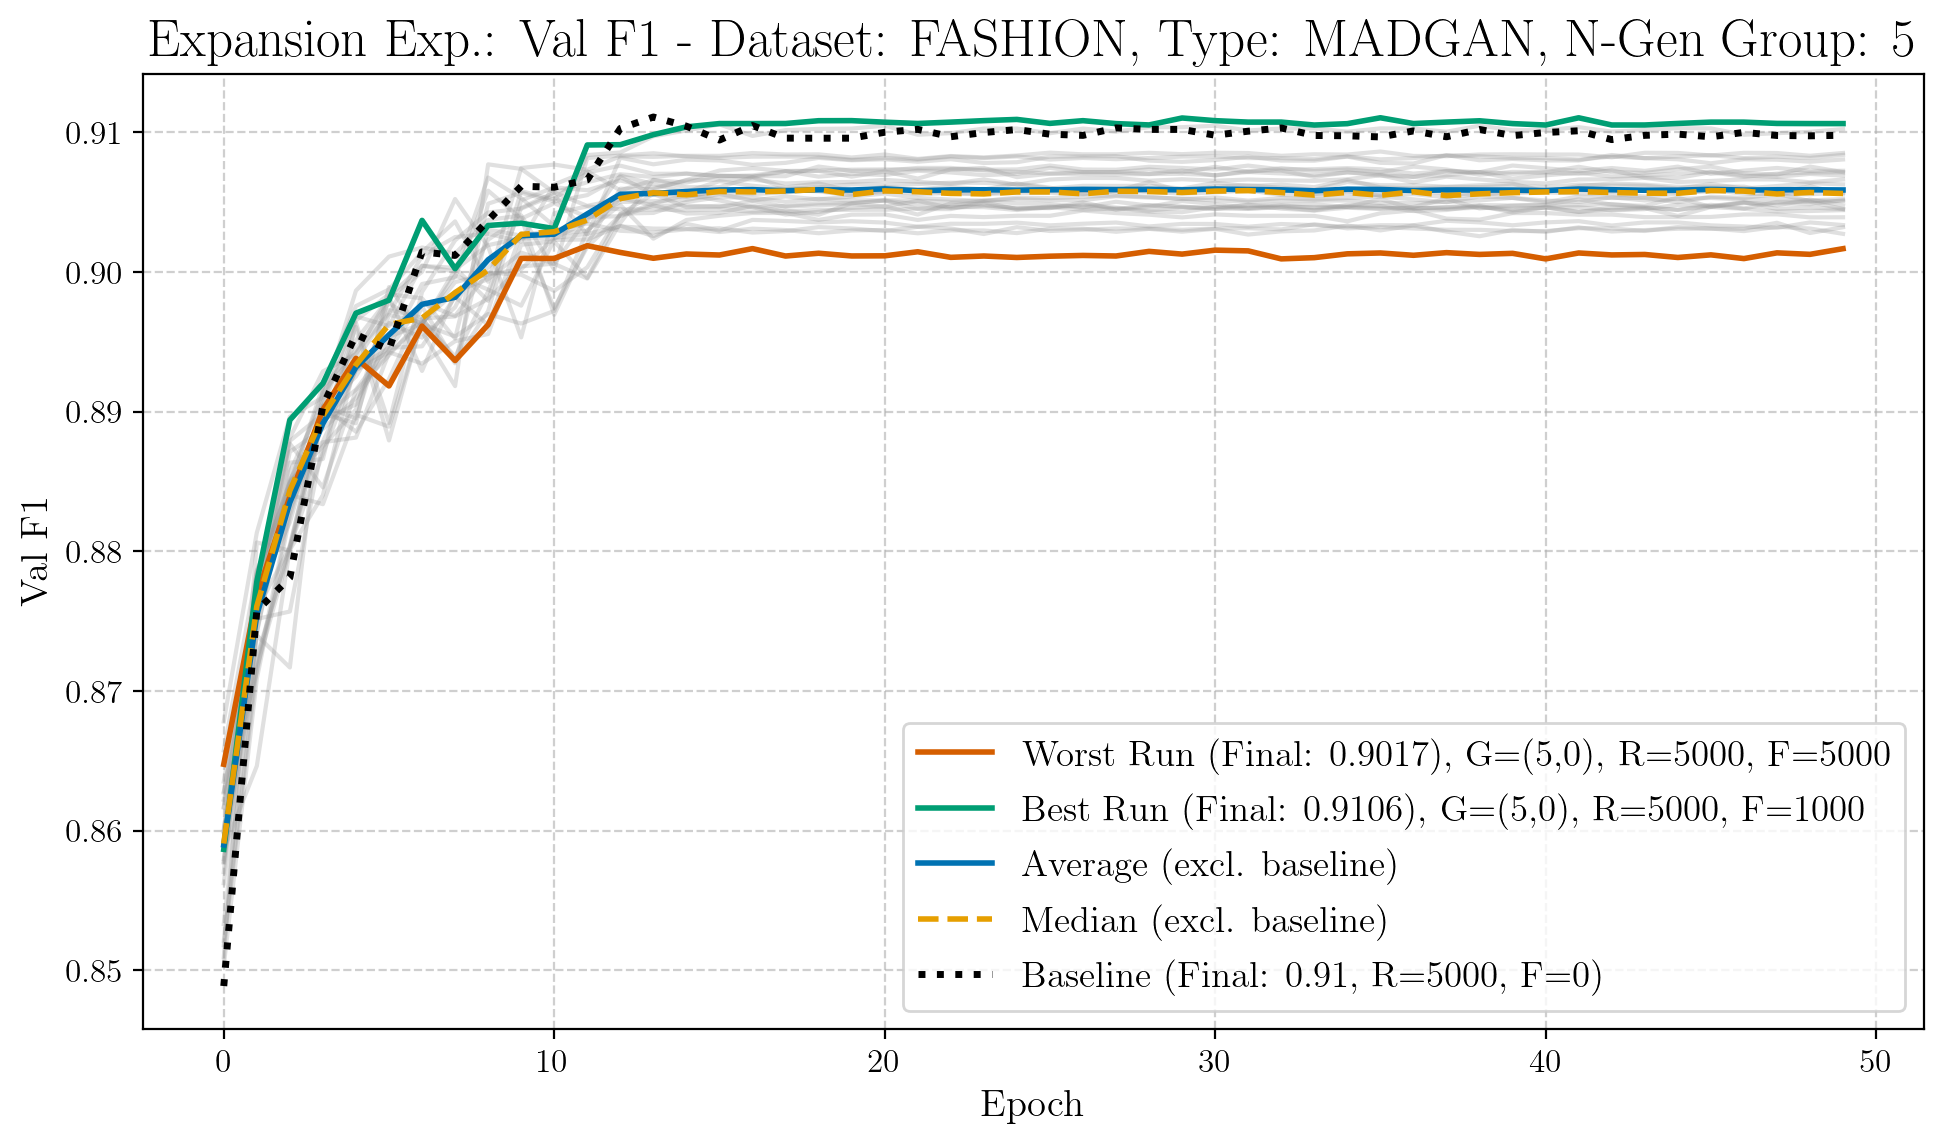
\includegraphics[width=.85\textwidth]{abb/strat_classifier_performance/FASHION_STRATIFIED_CLASSIFIERS_MADGAN_NEW/expansion_experiments/val_f1_score_MADGAN_FASHION_n_gen_5_all.png}
	\label{fig:app_strat_class_performance_expansion_exp._val_f1_score_5}
\end{figure}
\begin{table}[H]
	\vspace{-1em}
	\centering
	\begin{tabular}{|c|c|c|c|}
		\hline
		Run Type & Experiment & Val F1 \\ \hline
		best & \(G_{5, 0}\), R:5000, F:1000 & $0.9106$\\ \hline
		worst & \(G_{5, 0}\), R:5000, F:5000 & $0.9017$\\ \hline
		median & G (K=5) & $0.9056$\\ \hline
		average & G (K=5) & $0.9059$
		\\ \hline
	\end{tabular}
\end{table}
% End LaTeX Table for Expansion Experiment:
% LaTeX Metrics Table for Replacement Experiment: - Metric: val_f1_score - Target Gen Group: 5
\noindent\textbf{Replacement Experiment: K=5}
\begin{figure}[htbp]
	\centering
	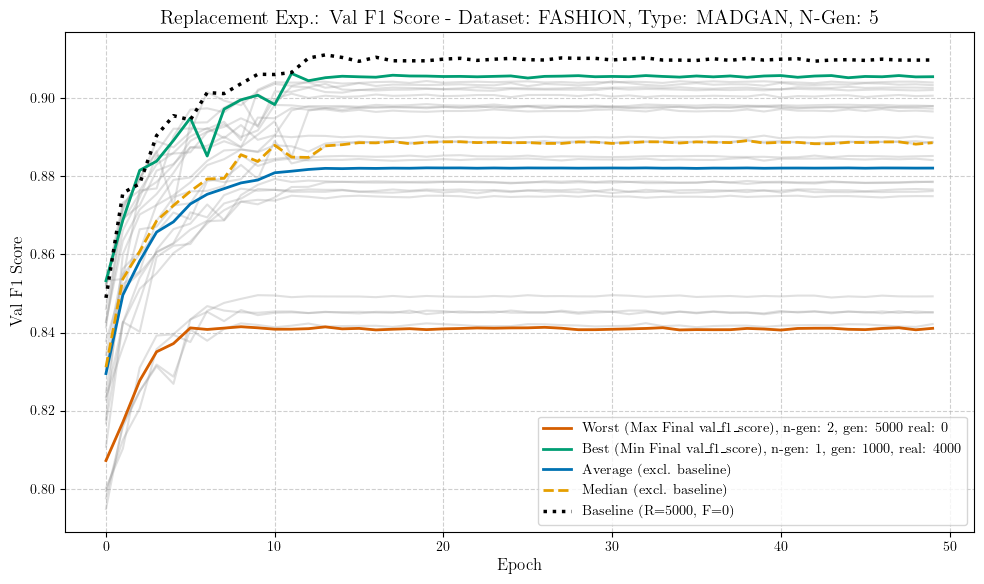
\includegraphics[width=.85\textwidth]{abb/strat_classifier_performance/FASHION_STRATIFIED_CLASSIFIERS_MADGAN_NEW/replacement_experiments/val_f1_score_MADGAN_FASHION_n_gen_5_all.png}
	\label{fig:app_strat_class_performance_replacement_exp._val_f1_score_5}
\end{figure}
\begin{table}[H]
	\vspace{-1em}
	\centering
	\begin{tabular}{|c|c|c|c|}
		\hline
		Run Type & Experiment & Val F1 \\ \hline
		best & \(G_{5, 1}\), R:4000, F:1000 & $0.9055$\\ \hline
		worst & \(G_{5, 2}\), R:0, F:5000 & $0.8411$\\ \hline
		median & G (K=5) & $0.8886$\\ \hline
		average & G (K=5) & $0.8821$
		\\ \hline
	\end{tabular}
\end{table}
% End LaTeX Table for Replacement Experiment:
\newpage
% LaTeX Metrics Table for Expansion Experiment: - Metric: val_f1_score - Target Gen Group: 7
\noindent\textbf{Expansion Experiment: K=7}
\begin{figure}[htbp]
	\centering
	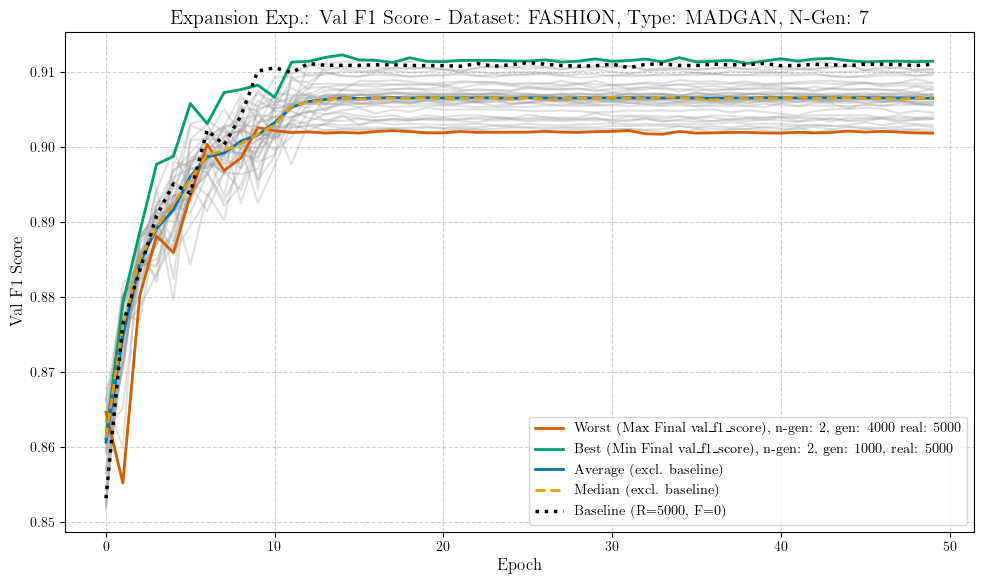
\includegraphics[width=.85\textwidth]{abb/strat_classifier_performance/FASHION_STRATIFIED_CLASSIFIERS_MADGAN_NEW/expansion_experiments/val_f1_score_MADGAN_FASHION_n_gen_7_all.png}
	\label{fig:app_strat_class_performance_expansion_exp._val_f1_score_7}
\end{figure}
\begin{table}[H]
	\vspace{-1em}
	\centering
	\begin{tabular}{|c|c|c|c|}
		\hline
		Run Type & Experiment & Val F1 \\ \hline
		best & \(G_{7, 2}\), R:5000, F:1000 & $0.9114$\\ \hline
		worst & \(G_{7, 2}\), R:5000, F:4000 & $0.9018$\\ \hline
		median & G (K=7) & $0.9066$\\ \hline
		average & G (K=7) & $0.9065$
		\\ \hline
	\end{tabular}
\end{table}
% End LaTeX Table for Expansion Experiment:
% LaTeX Metrics Table for Replacement Experiment: - Metric: val_f1_score - Target Gen Group: 7
\noindent\textbf{Replacement Experiment: K=7}
\begin{figure}[htbp]
	\centering
	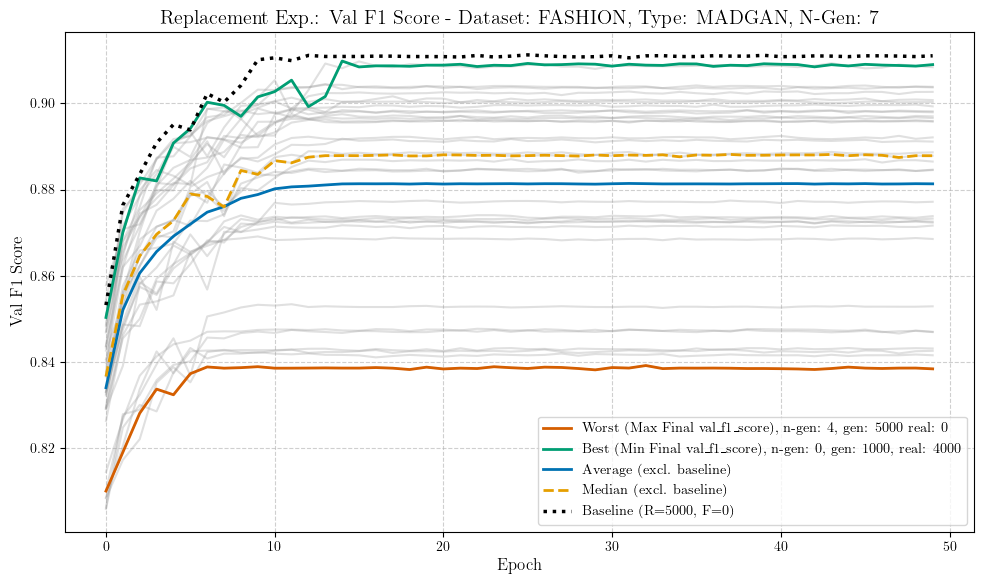
\includegraphics[width=.85\textwidth]{abb/strat_classifier_performance/FASHION_STRATIFIED_CLASSIFIERS_MADGAN_NEW/replacement_experiments/val_f1_score_MADGAN_FASHION_n_gen_7_all.png}
	\label{fig:app_strat_class_performance_replacement_exp._val_f1_score_7}
\end{figure}
\begin{table}[H]
	\vspace{-1em}
	\centering
	\begin{tabular}{|c|c|c|c|}
		\hline
		Run Type & Experiment & Val F1 \\ \hline
		best & \(G_{7, 0}\), R:4000, F:1000 & $0.9090$\\ \hline
		worst & \(G_{7, 4}\), R:0, F:5000 & $0.8384$\\ \hline
		median & G (K=7) & $0.8879$\\ \hline
		average & G (K=7) & $0.8813$
		\\ \hline
	\end{tabular}
\end{table}
% End LaTeX Table for Replacement Experiment:
\newpage
% LaTeX Metrics Table for Expansion Experiment: - Metric: val_f1_score - Target Gen Group: 10
\noindent\textbf{Expansion Experiment: K=10}
\begin{figure}[htbp]
	\centering
	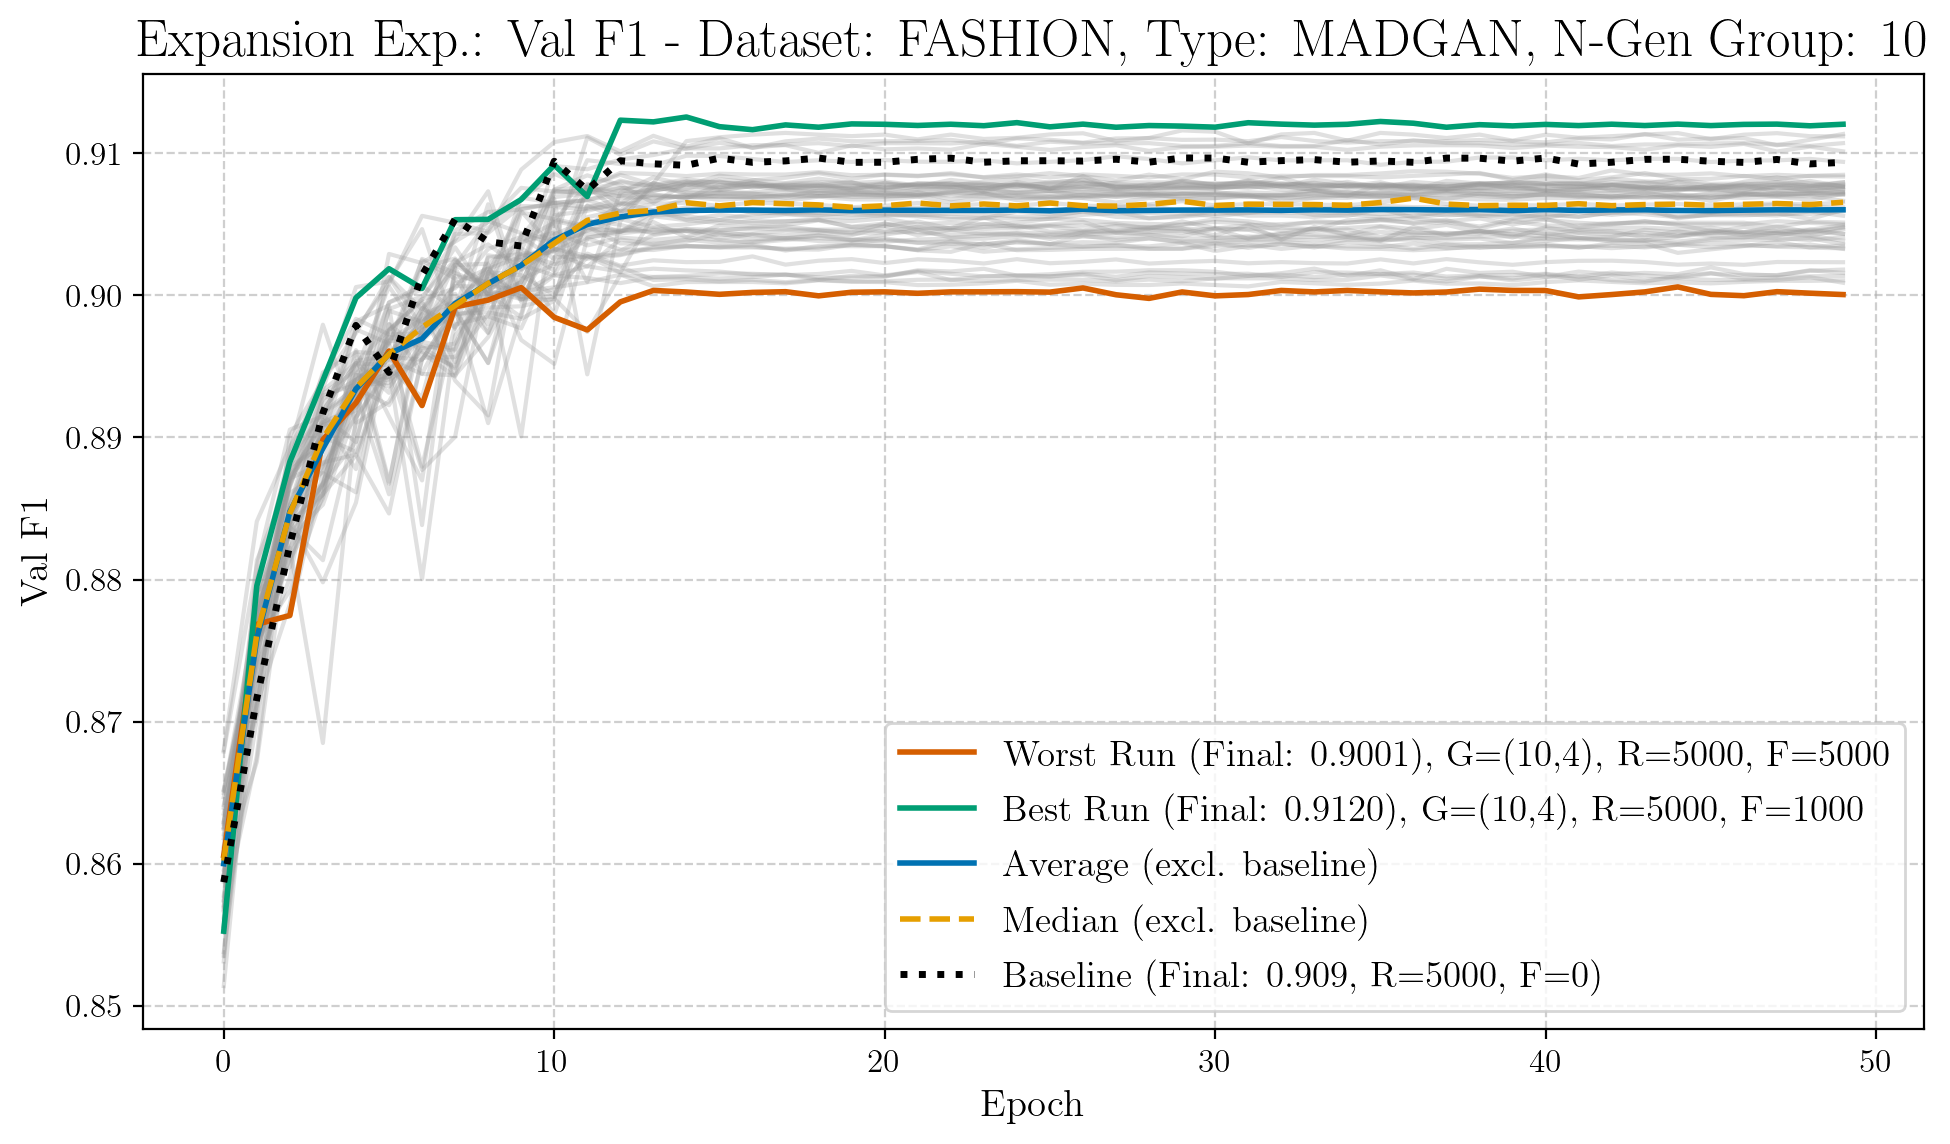
\includegraphics[width=.85\textwidth]{abb/strat_classifier_performance/FASHION_STRATIFIED_CLASSIFIERS_MADGAN_NEW/expansion_experiments/val_f1_score_MADGAN_FASHION_n_gen_10_all.png}
	\label{fig:app_strat_class_performance_expansion_exp._val_f1_score_10}
\end{figure}
\begin{table}[H]
	\vspace{-1em}
	\centering
	\begin{tabular}{|c|c|c|c|}
		\hline
		Run Type & Experiment & Val F1 \\ \hline
		best & \(G_{10, 4}\), R:5000, F:1000 & $0.9120$\\ \hline
		worst & \(G_{10, 4}\), R:5000, F:5000 & $0.9001$\\ \hline
		median & G (K=10) & $0.9066$\\ \hline
		average & G (K=10) & $0.9060$
		\\ \hline
	\end{tabular}
\end{table}
% End LaTeX Table for Expansion Experiment:
% LaTeX Metrics Table for Replacement Experiment: - Metric: val_f1_score - Target Gen Group: 10
\noindent\textbf{Replacement Experiment: K=10}
\begin{figure}[htbp]
	\centering
	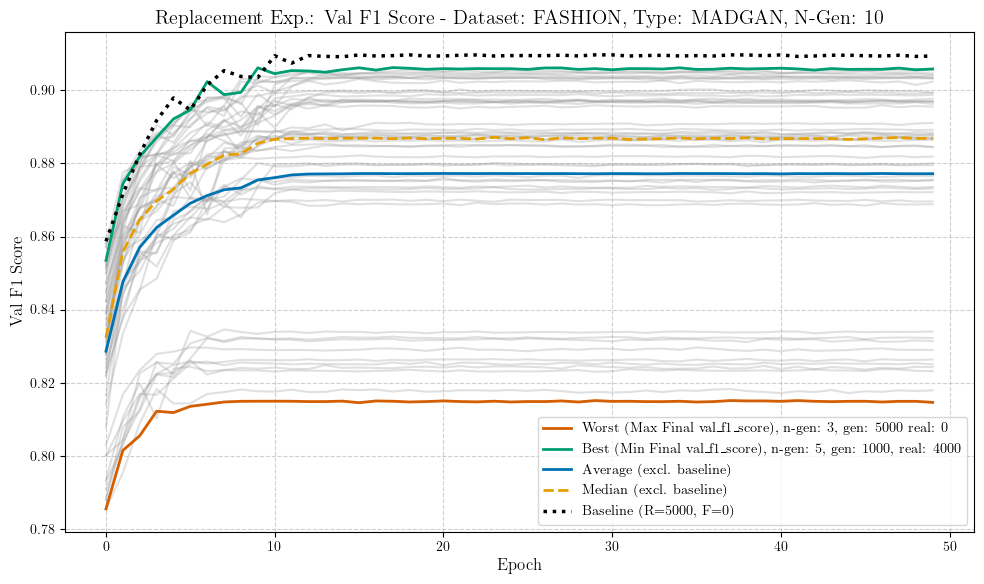
\includegraphics[width=.85\textwidth]{abb/strat_classifier_performance/FASHION_STRATIFIED_CLASSIFIERS_MADGAN_NEW/replacement_experiments/val_f1_score_MADGAN_FASHION_n_gen_10_all.png}
	\label{fig:app_strat_class_performance_replacement_exp._val_f1_score_10}
\end{figure}
\begin{table}[H]
	\vspace{-1em}
	\centering
	\begin{tabular}{|c|c|c|c|}
		\hline
		Run Type & Experiment & Val F1 \\ \hline
		best & \(G_{10, 5}\), R:4000, F:1000 & $0.9058$\\ \hline
		worst & \(G_{10, 3}\), R:0, F:5000 & $0.8146$\\ \hline
		median & G (K=10) & $0.8869$\\ \hline
		average & G (K=10) & $0.8772$
		\\ \hline
	\end{tabular}
\end{table}
% End LaTeX Table for Replacement Experiment:
\newpage
\subsubsection{Dataset: FASHION, Architecture: cMADGAN}
% LaTeX Metrics Table for Expansion Experiment: - Metric: val_f1_score - Target Gen Group: 3
\noindent\textbf{Expansion Experiment: K=3}
\begin{figure}[htbp]
	\centering
	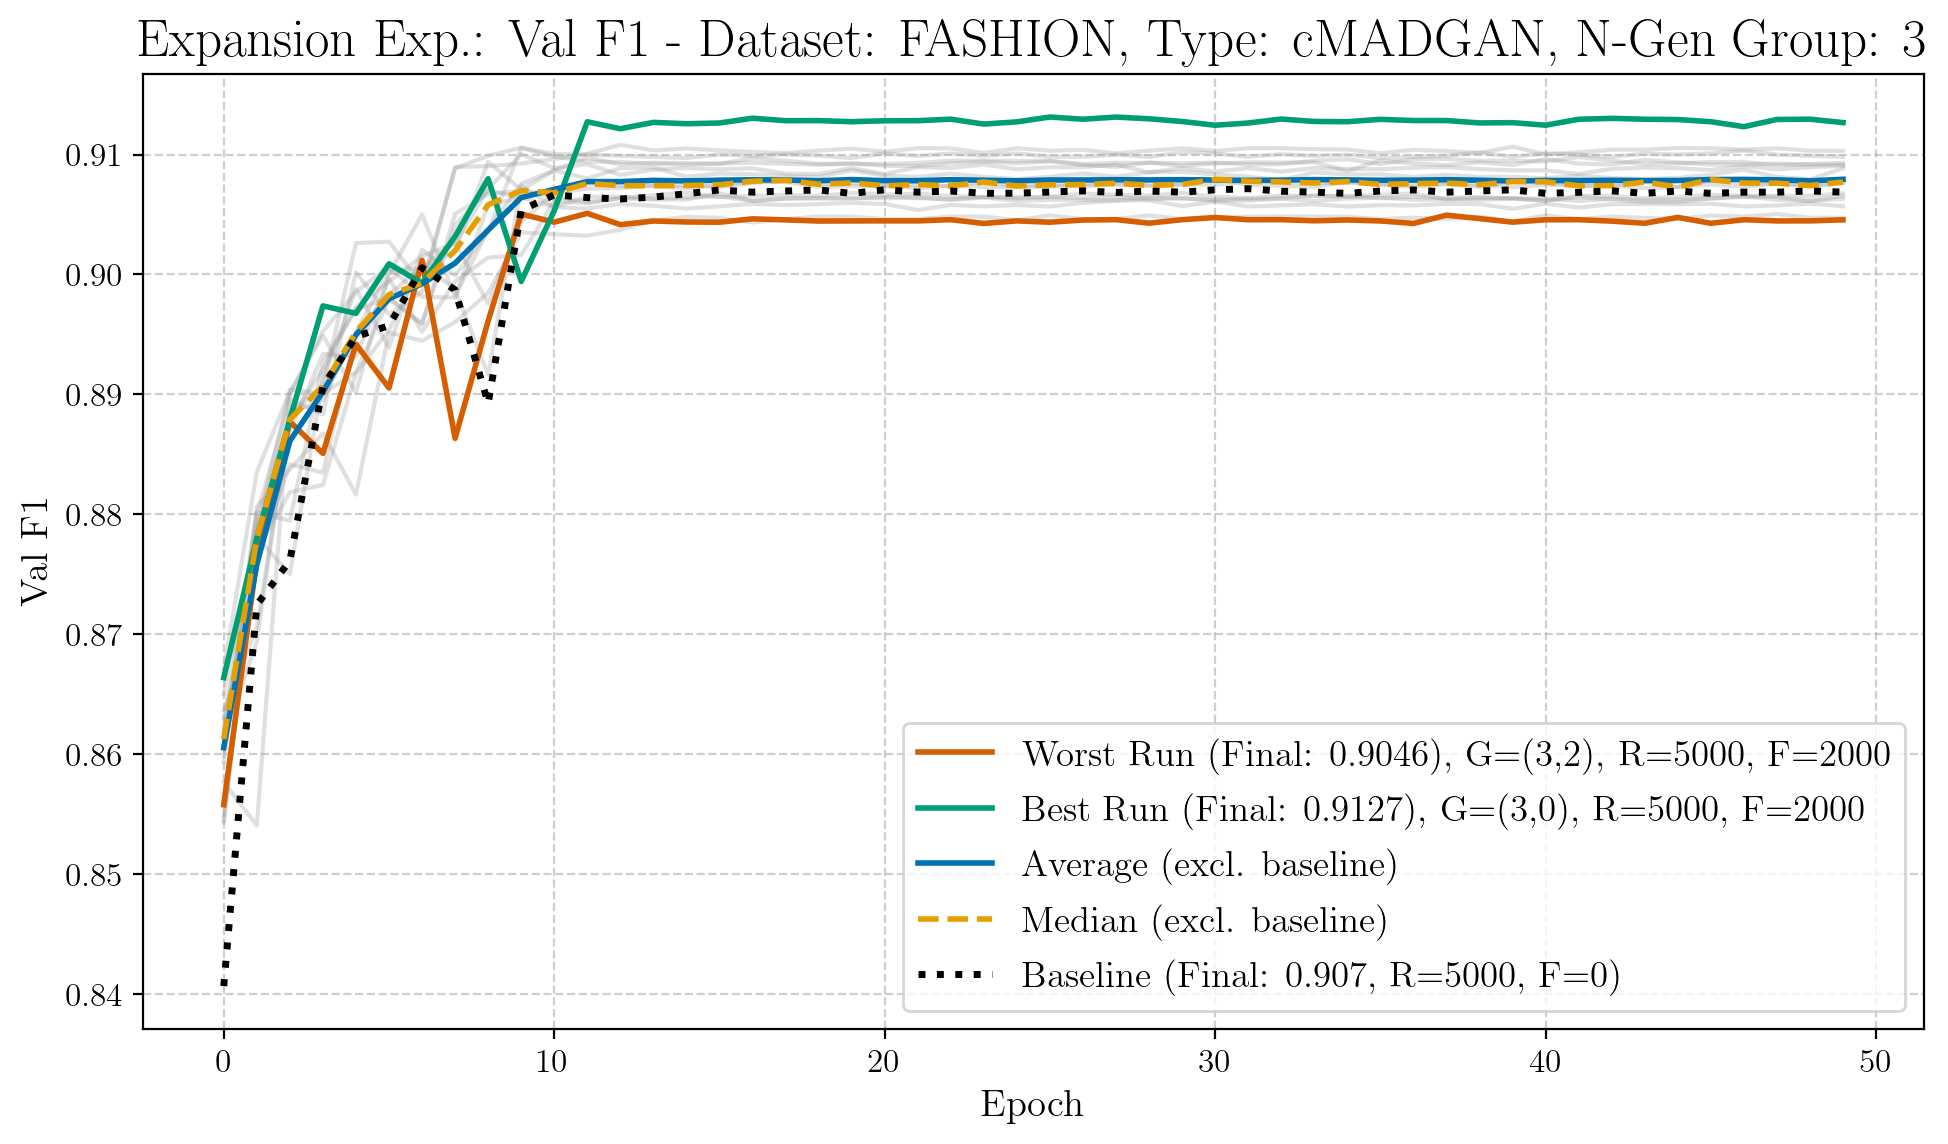
\includegraphics[width=.85\textwidth]{abb/strat_classifier_performance/FASHION_STRATIFIED_CLASSIFIERS_cMADGAN_NEW/expansion_experiments/val_f1_score_cMADGAN_FASHION_n_gen_3_all.png}
	\label{fig:app_strat_class_performance_expansion_exp._val_f1_score_3}
\end{figure}
\begin{table}[H]
	\vspace{-1em}
	\centering
	\begin{tabular}{|c|c|c|c|}
		\hline
		Run Type & Experiment & Val F1 \\ \hline
		best & \(G_{3, 0}\), R:5000, F:2000 & $0.9127$\\ \hline
		worst & \(G_{3, 2}\), R:5000, F:2000 & $0.9046$\\ \hline
		median & G (K=3) & $0.9077$\\ \hline
		average & G (K=3) & $0.9079$
		\\ \hline
	\end{tabular}
\end{table}
% End LaTeX Table for Expansion Experiment:
% LaTeX Metrics Table for Replacement Experiment: - Metric: val_f1_score - Target Gen Group: 3
\noindent\textbf{Replacement Experiment: K=3}
\begin{figure}[htbp]
	\centering
	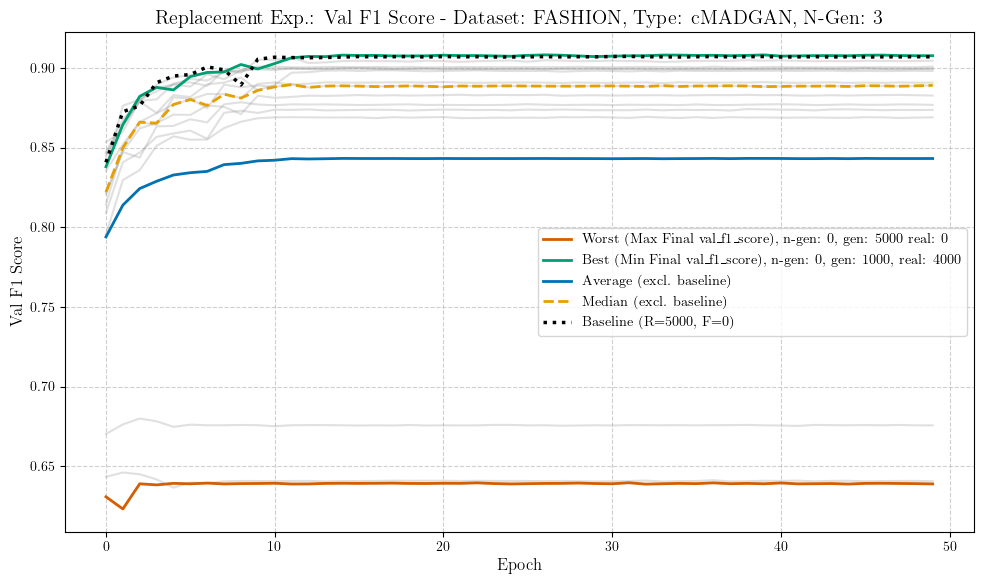
\includegraphics[width=.85\textwidth]{abb/strat_classifier_performance/FASHION_STRATIFIED_CLASSIFIERS_cMADGAN_NEW/replacement_experiments/val_f1_score_cMADGAN_FASHION_n_gen_3_all.png}
	\label{fig:app_strat_class_performance_replacement_exp._val_f1_score_3}
\end{figure}
\begin{table}[H]
	\vspace{-1em}
	\centering
	\begin{tabular}{|c|c|c|c|}
		\hline
		Run Type & Experiment & Val F1 \\ \hline
		best & \(G_{3, 0}\), R:4000, F:1000 & $0.9076$\\ \hline
		worst & \(G_{3, 0}\), R:0, F:5000 & $0.6390$\\ \hline
		median & G (K=3) & $0.8890$\\ \hline
		average & G (K=3) & $0.8431$
		\\ \hline
	\end{tabular}
\end{table}
% End LaTeX Table for Replacement Experiment:
\newpage
% LaTeX Metrics Table for Expansion Experiment: - Metric: val_f1_score - Target Gen Group: 5
\noindent\textbf{Expansion Experiment: K=5}
\begin{figure}[htbp]
	\centering
	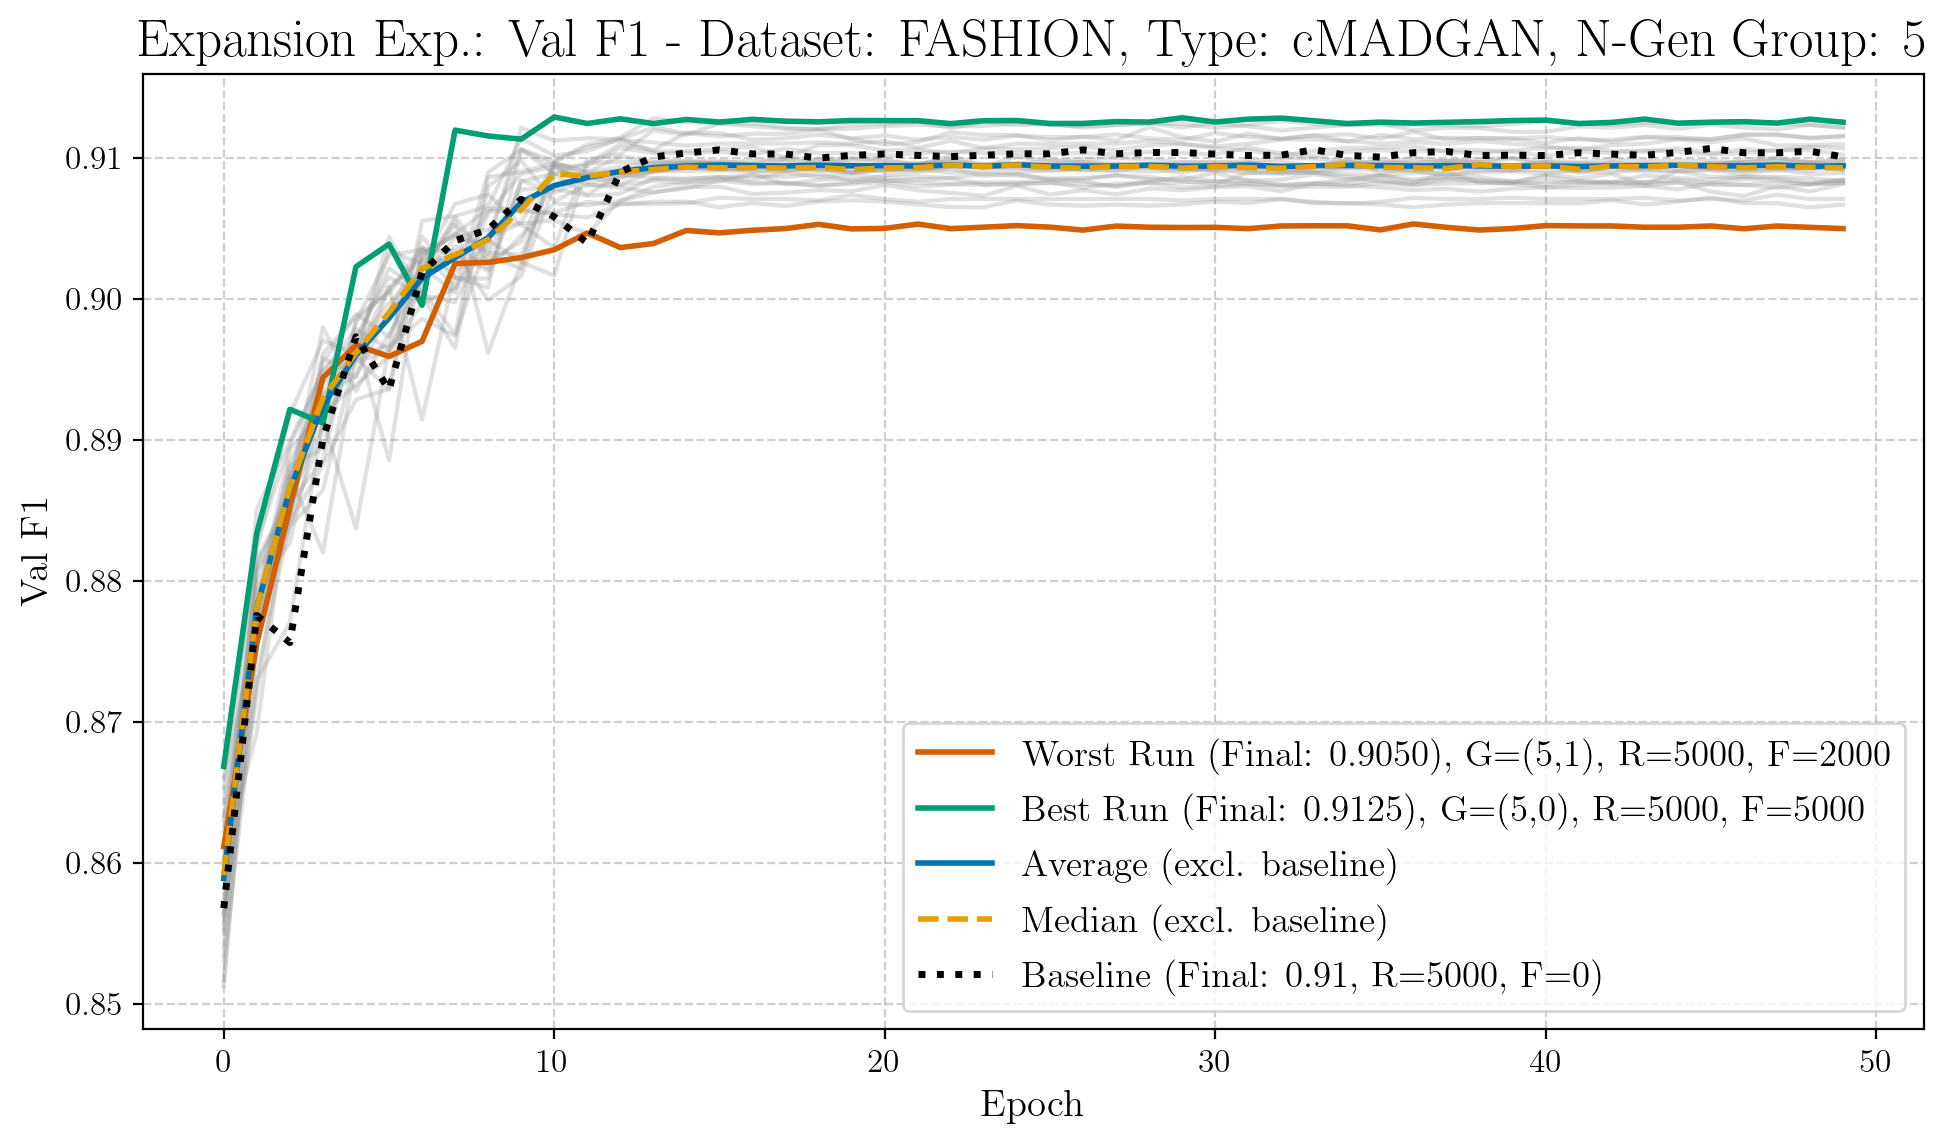
\includegraphics[width=.85\textwidth]{abb/strat_classifier_performance/FASHION_STRATIFIED_CLASSIFIERS_cMADGAN_NEW/expansion_experiments/val_f1_score_cMADGAN_FASHION_n_gen_5_all.png}
	\label{fig:app_strat_class_performance_expansion_exp._val_f1_score_5}
\end{figure}
\begin{table}[H]
	\vspace{-1em}
	\centering
	\begin{tabular}{|c|c|c|c|}
		\hline
		Run Type & Experiment & Val F1 \\ \hline
		best & \(G_{5, 0}\), R:5000, F:5000 & $0.9125$\\ \hline
		worst & \(G_{5, 1}\), R:5000, F:2000 & $0.9050$\\ \hline
		median & G (K=5) & $0.9093$\\ \hline
		average & G (K=5) & $0.9094$
		\\ \hline
	\end{tabular}
\end{table}
% End LaTeX Table for Expansion Experiment:
% LaTeX Metrics Table for Replacement Experiment: - Metric: val_f1_score - Target Gen Group: 5
\noindent\textbf{Replacement Experiment: K=5}
\begin{figure}[htbp]
	\centering
	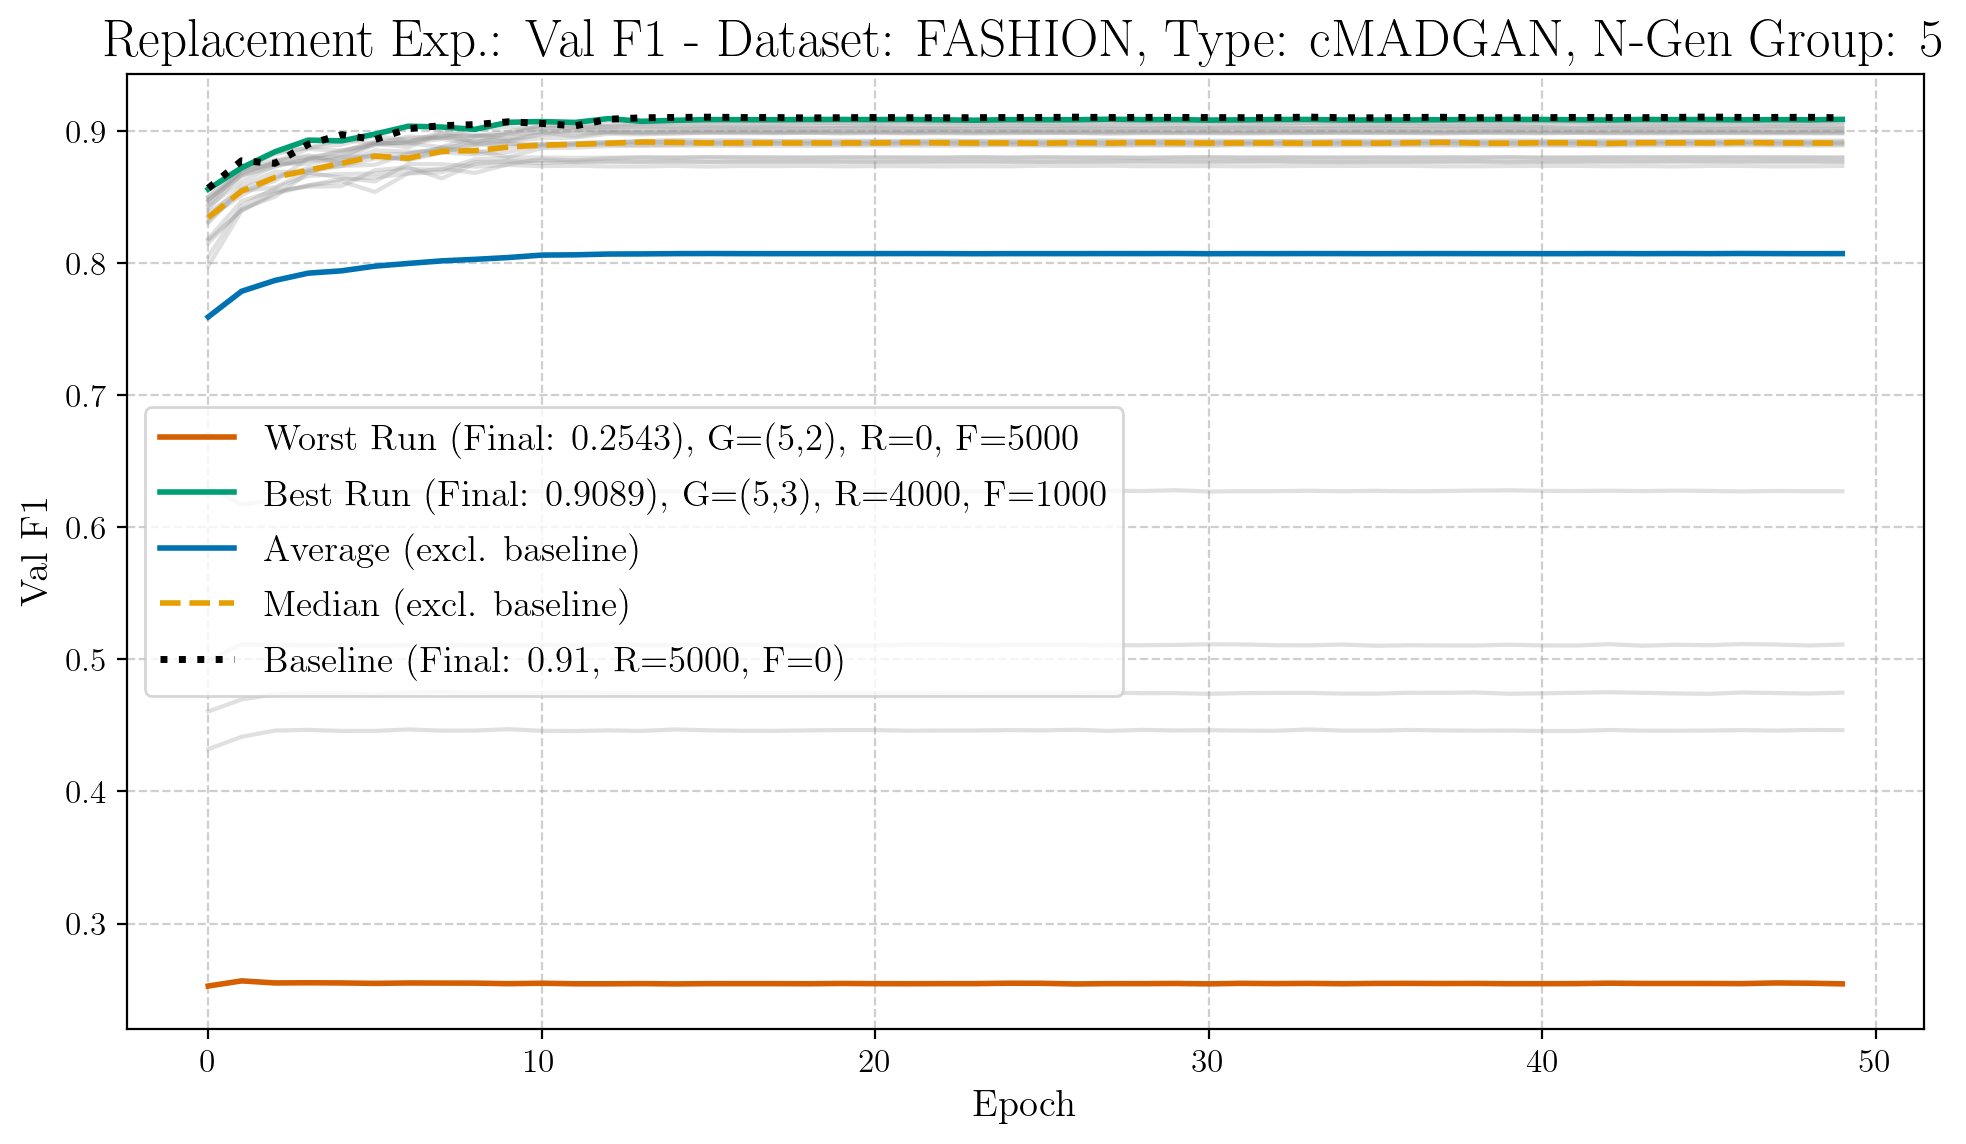
\includegraphics[width=.85\textwidth]{abb/strat_classifier_performance/FASHION_STRATIFIED_CLASSIFIERS_cMADGAN_NEW/replacement_experiments/val_f1_score_cMADGAN_FASHION_n_gen_5_all.png}
	\label{fig:app_strat_class_performance_replacement_exp._val_f1_score_5}
\end{figure}
\begin{table}[H]
	\vspace{-1em}
	\centering
	\begin{tabular}{|c|c|c|c|}
		\hline
		Run Type & Experiment & Val F1 \\ \hline
		best & \(G_{5, 3}\), R:4000, F:1000 & $0.9089$\\ \hline
		worst & \(G_{5, 2}\), R:0, F:5000 & $0.2543$\\ \hline
		median & G (K=5) & $0.8909$\\ \hline
		average & G (K=5) & $0.8072$
		\\ \hline
	\end{tabular}
\end{table}
% End LaTeX Table for Replacement Experiment:
\newpage
% LaTeX Metrics Table for Expansion Experiment: - Metric: val_f1_score - Target Gen Group: 7
\noindent\textbf{Expansion Experiment: K=7}
\begin{figure}[htbp]
	\centering
	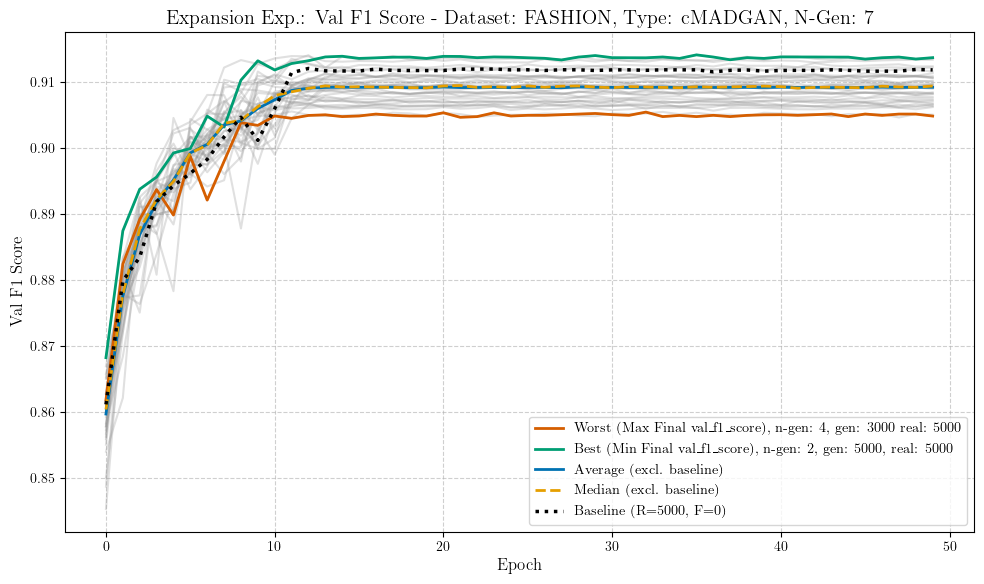
\includegraphics[width=.85\textwidth]{abb/strat_classifier_performance/FASHION_STRATIFIED_CLASSIFIERS_cMADGAN_NEW/expansion_experiments/val_f1_score_cMADGAN_FASHION_n_gen_7_all.png}
	\label{fig:app_strat_class_performance_expansion_exp._val_f1_score_7}
\end{figure}
\begin{table}[H]
	\vspace{-1em}
	\centering
	\begin{tabular}{|c|c|c|c|}
		\hline
		Run Type & Experiment & Val F1 \\ \hline
		best & \(G_{7, 2}\), R:5000, F:5000 & $0.9138$\\ \hline
		worst & \(G_{7, 4}\), R:5000, F:3000 & $0.9049$\\ \hline
		median & G (K=7) & $0.9095$\\ \hline
		average & G (K=7) & $0.9093$
		\\ \hline
	\end{tabular}
\end{table}
% End LaTeX Table for Expansion Experiment:
% LaTeX Metrics Table for Replacement Experiment: - Metric: val_f1_score - Target Gen Group: 7
\noindent\textbf{Replacement Experiment: K=7}
\begin{figure}[htbp]
	\centering
	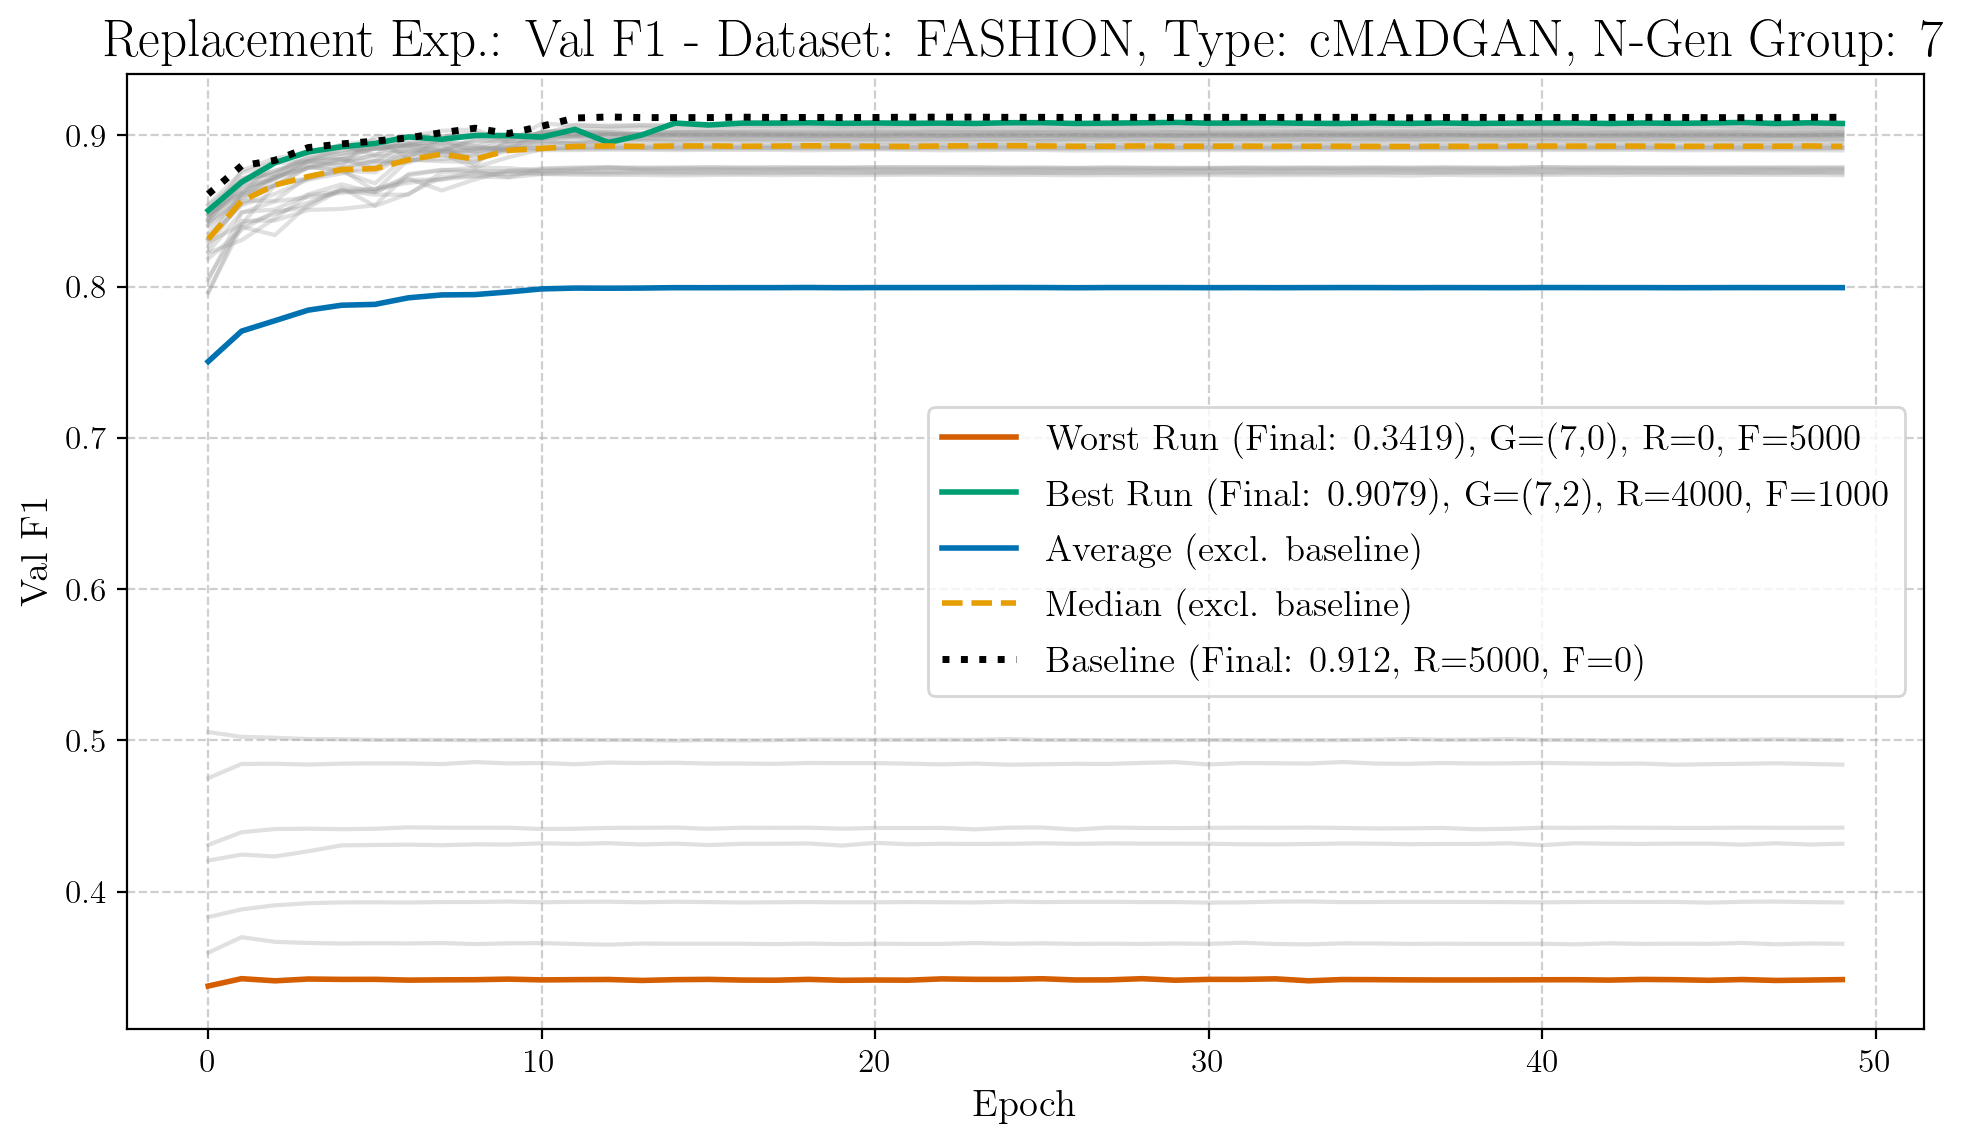
\includegraphics[width=.85\textwidth]{abb/strat_classifier_performance/FASHION_STRATIFIED_CLASSIFIERS_cMADGAN_NEW/replacement_experiments/val_f1_score_cMADGAN_FASHION_n_gen_7_all.png}
	\label{fig:app_strat_class_performance_replacement_exp._val_f1_score_7}
\end{figure}
\begin{table}[H]
	\vspace{-1em}
	\centering
	\begin{tabular}{|c|c|c|c|}
		\hline
		Run Type & Experiment & Val F1 \\ \hline
		best & \(G_{7, 2}\), R:4000, F:1000 & $0.9079$\\ \hline
		worst & \(G_{7, 0}\), R:0, F:5000 & $0.3419$\\ \hline
		median & G (K=7) & $0.8927$\\ \hline
		average & G (K=7) & $0.7993$
		\\ \hline
	\end{tabular}
\end{table}
% End LaTeX Table for Replacement Experiment:
\newpage
% LaTeX Metrics Table for Expansion Experiment: - Metric: val_f1_score - Target Gen Group: 10
\noindent\textbf{Expansion Experiment: K=10}
\begin{figure}[htbp]
	\centering
	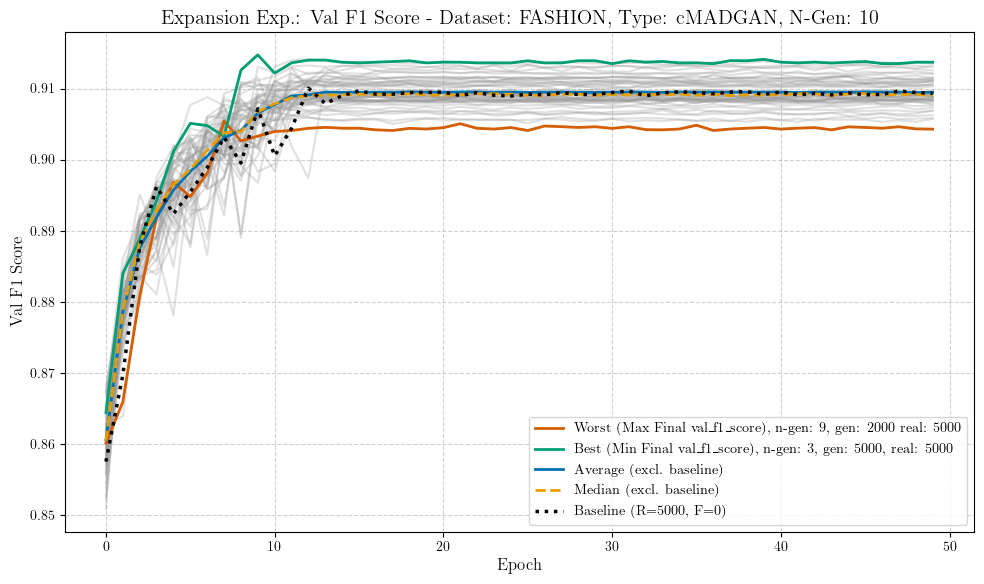
\includegraphics[width=.85\textwidth]{abb/strat_classifier_performance/FASHION_STRATIFIED_CLASSIFIERS_cMADGAN_NEW/expansion_experiments/val_f1_score_cMADGAN_FASHION_n_gen_10_all.png}
	\label{fig:app_strat_class_performance_expansion_exp._val_f1_score_10}
\end{figure}
\begin{table}[H]
	\vspace{-1em}
	\centering
	\begin{tabular}{|c|c|c|c|}
		\hline
		Run Type & Experiment & Val F1 \\ \hline
		best & \(G_{10, 3}\), R:5000, F:5000 & $0.9137$\\ \hline
		worst & \(G_{10, 9}\), R:5000, F:2000 & $0.9043$\\ \hline
		median & G (K=10) & $0.9091$\\ \hline
		average & G (K=10) & $0.9095$
		\\ \hline
	\end{tabular}
\end{table}
% End LaTeX Table for Expansion Experiment:
% LaTeX Metrics Table for Replacement Experiment: - Metric: val_f1_score - Target Gen Group: 10
\noindent\textbf{Replacement Experiment: K=10}
\begin{figure}[htbp]
	\centering
	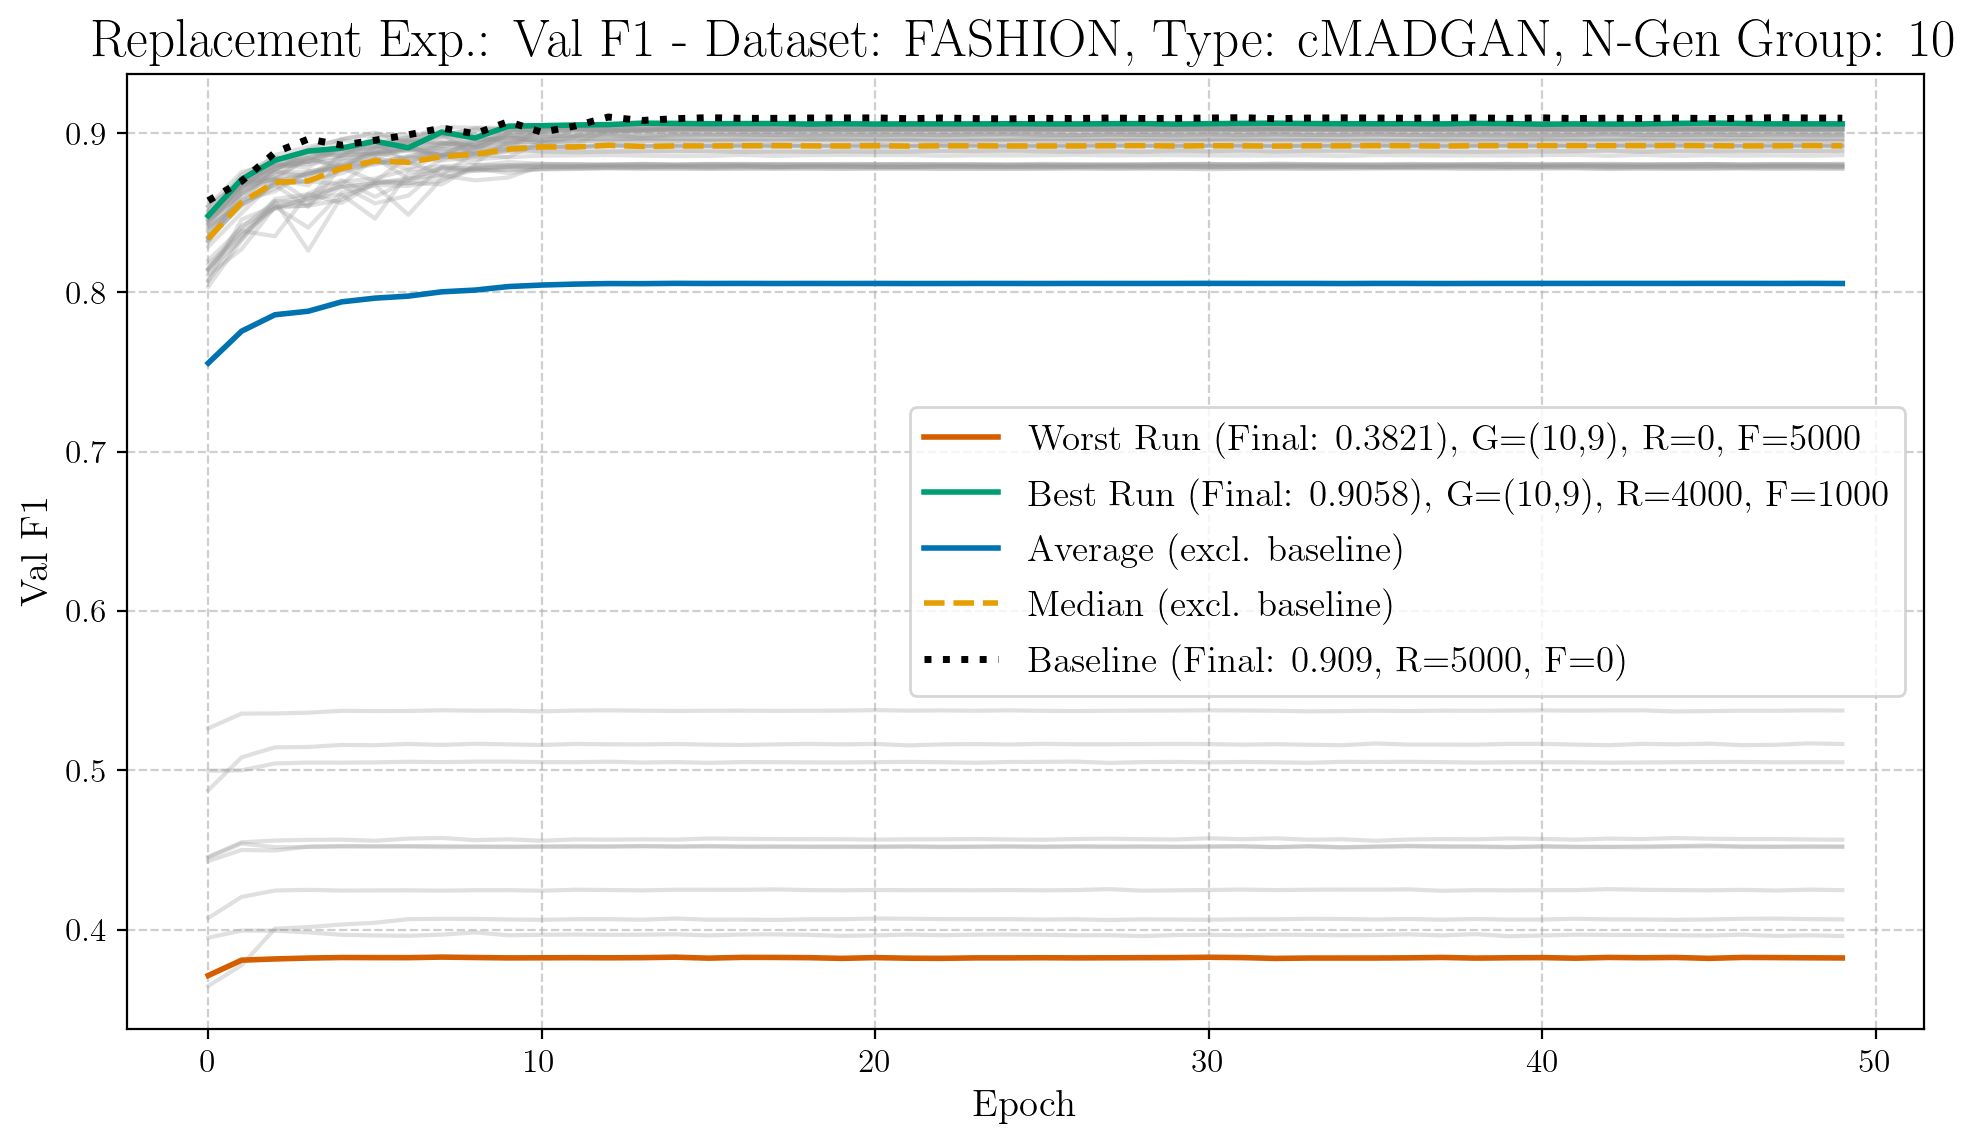
\includegraphics[width=.85\textwidth]{abb/strat_classifier_performance/FASHION_STRATIFIED_CLASSIFIERS_cMADGAN_NEW/replacement_experiments/val_f1_score_cMADGAN_FASHION_n_gen_10_all.png}
	\label{fig:app_strat_class_performance_replacement_exp._val_f1_score_10}
\end{figure}
\begin{table}[H]
	\vspace{-1em}
	\centering
	\begin{tabular}{|c|c|c|c|}
		\hline
		Run Type & Experiment & Val F1 \\ \hline
		best & \(G_{10, 9}\), R:4000, F:1000 & $0.9058$\\ \hline
		worst & \(G_{10, 9}\), R:0, F:5000 & $0.3821$\\ \hline
		median & G (K=10) & $0.8920$\\ \hline
		average & G (K=10) & $0.8056$
		\\ \hline
	\end{tabular}
\end{table}
% End LaTeX Table for Replacement Experiment:
\newpage

\subsubsection{Dataset: MNIST, Architecture: Deep Convolutional GAN}\label{app_STRAT_CLASS_PERF_mnist_DCGAN}
% LaTeX Metrics Table for Expansion Experiment: - Metric: val_f1_score
% LaTeX Metrics Table for Expansion Experiment: - Metric: val_f1_score - Target Gen Group: 10
\noindent\textbf{Expansion Experiment:}
\begin{figure}[htbp]
	\centering
	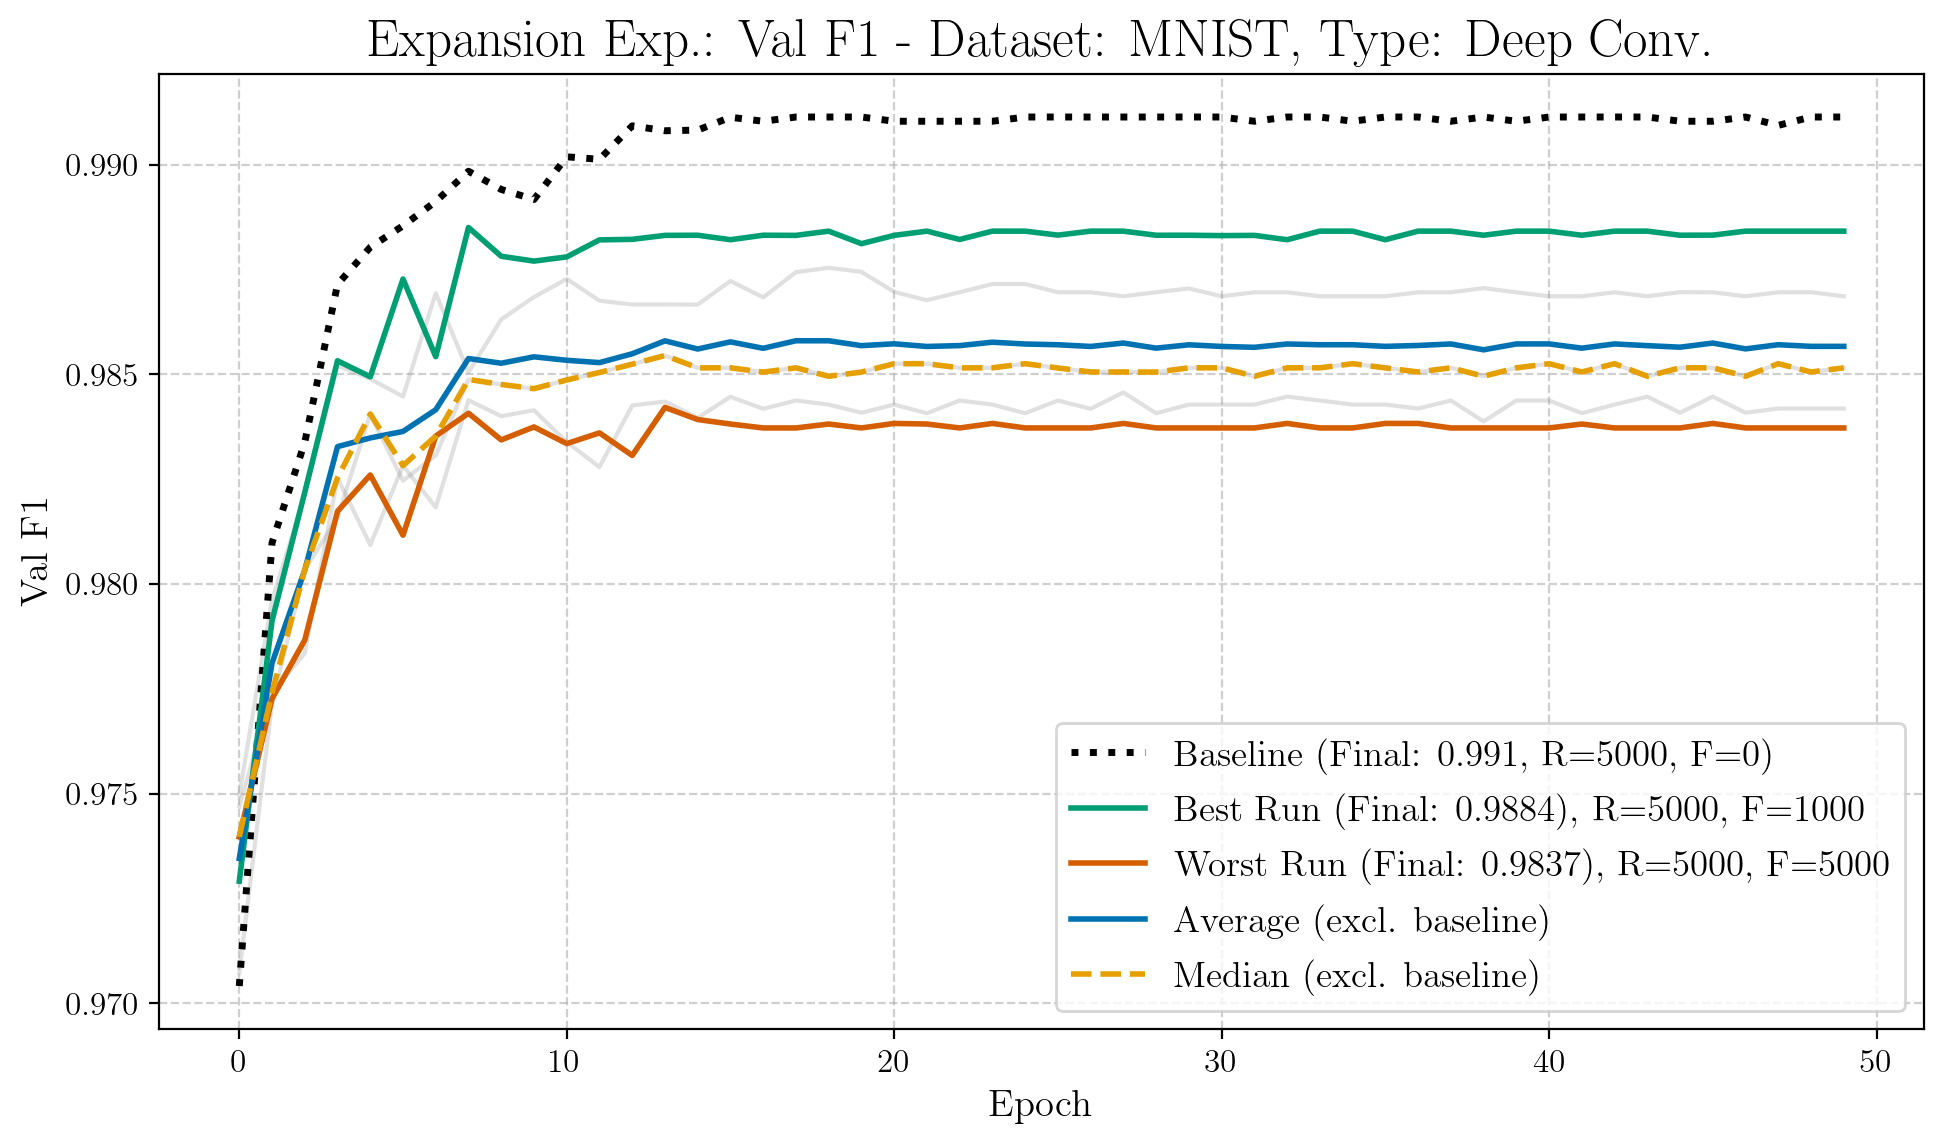
\includegraphics[width=.85\textwidth]{abb/strat_classifier_performance/MNIST_STRATIFIED_CLASSIFIERS_VANILLA_GAN/expansion_experiments/val_f1_score_['VANILLA']_MNIST_all.png}
	\label{fig:app_strat_class_performance_expansion_exp_val_f1_score_DCGAN}
\end{figure}
\begin{table}[H]
	\centering
	\vspace{-1em}
	\begin{tabular}{|c|c|c|c|c|}
		\hline
		Run Type & Experiment & Val F1 \\ \hline
		best & DC (R:5000, F:1000) & $0.9884$\\ \hline
		worst & DC (R:5000, F:5000) & $0.9837$\\ \hline
		median & DC & $0.9852$\\ \hline
		average & DC & $0.9857$
		\\ \hline
	\end{tabular}
\end{table}
% End LaTeX Table for Expansion Experiment:
% LaTeX Metrics Table for Replacement Experiment: - Metric: val_f1_score
% LaTeX Metrics Table for Replacement Experiment: - Metric: val_f1_score - Target Gen Group: 10
\noindent\textbf{Replacement Experiment:}
\begin{figure}[htbp]
	\centering
	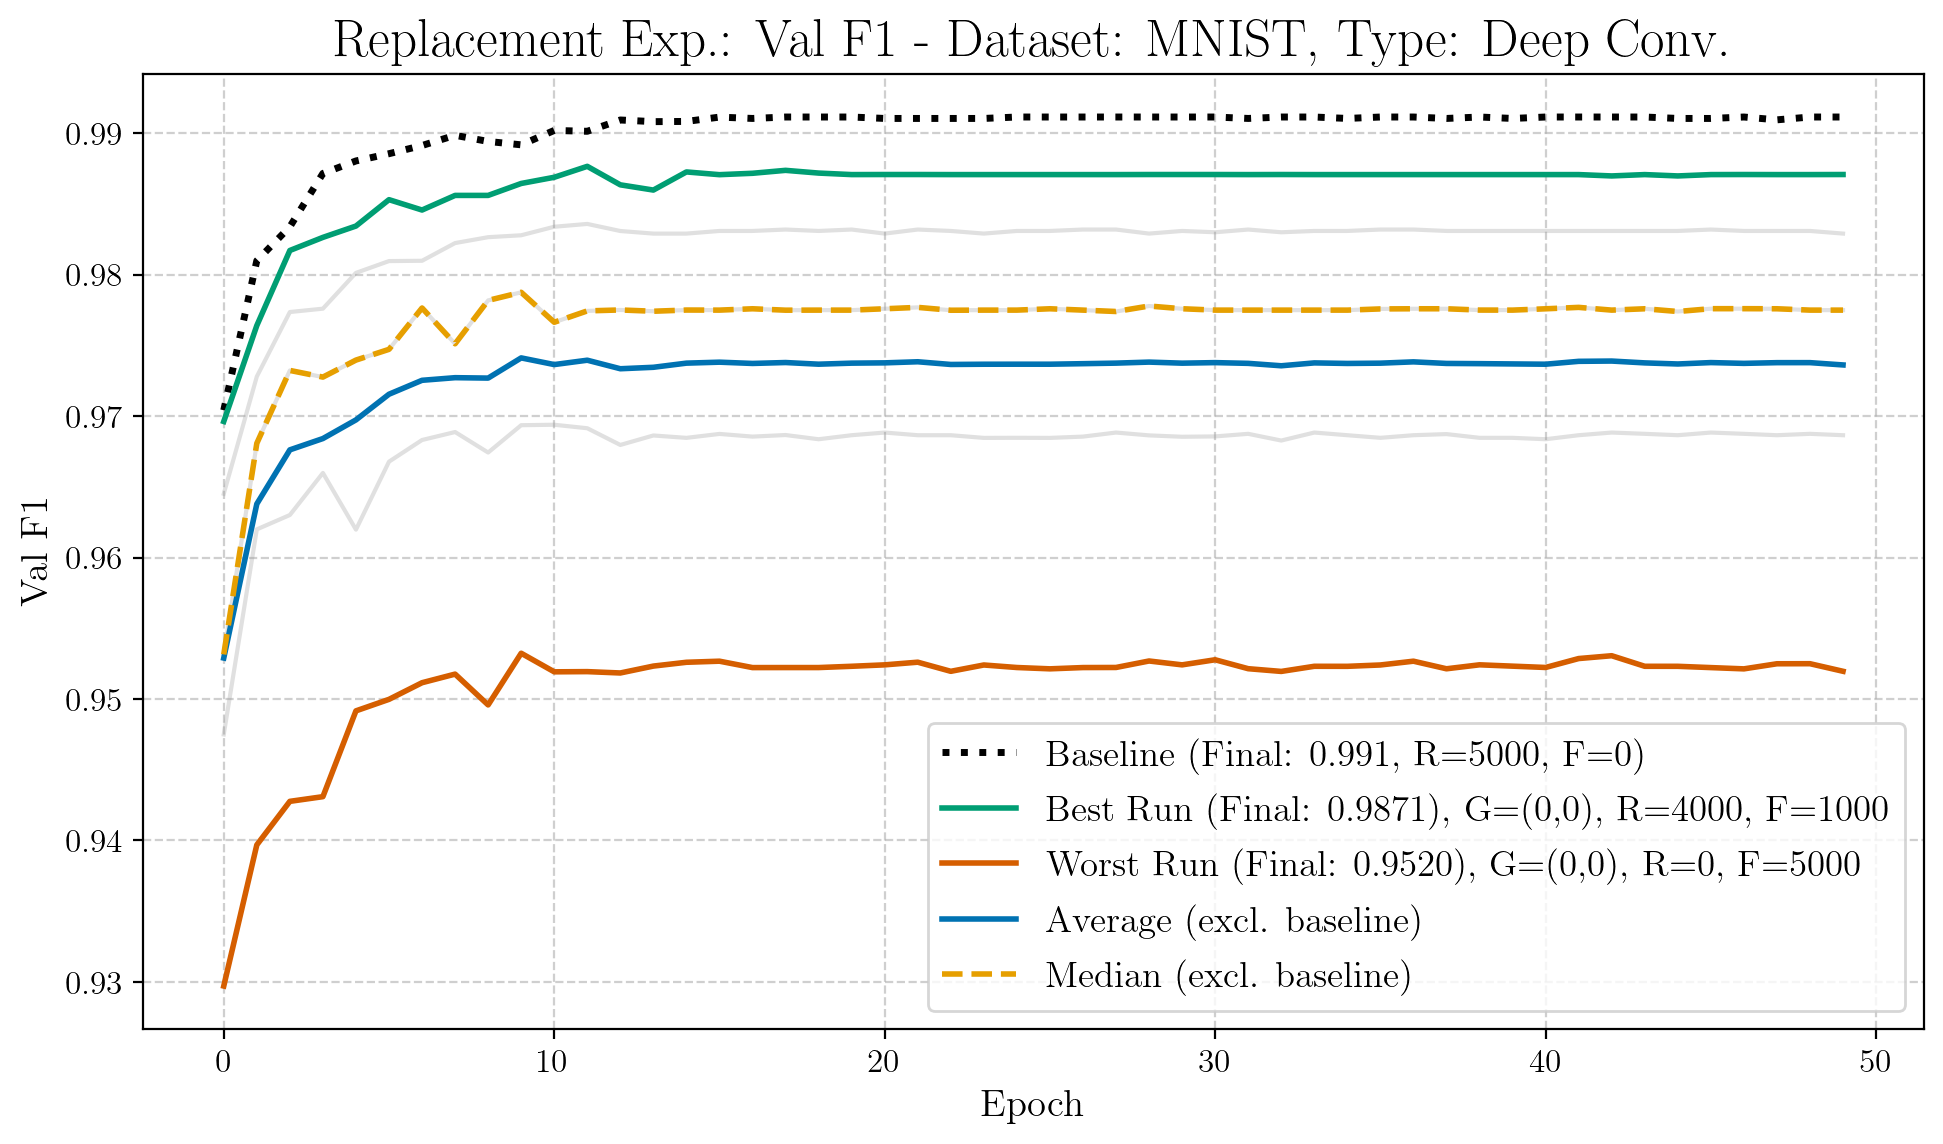
\includegraphics[width=.85\textwidth]{abb/strat_classifier_performance/MNIST_STRATIFIED_CLASSIFIERS_VANILLA_GAN/replacement_experiments/val_f1_score_['VANILLA']_MNIST_all.png}
	\label{fig:app_strat_class_performance_replacement_exp._val_f1_score_DCGAN}
\end{figure}
\begin{table}[H]
	\centering
	\vspace{-1em}
	\begin{tabular}{|c|c|c|c|c|}
		\hline
		Run Type & Experiment & Val F1 \\ \hline
		best & DC (R:4000:, F:1000) & $0.9871$\\ \hline
		worst & DC (R:0, F:5000) & $0.9520$\\ \hline
		median & DC & $0.9775$\\ \hline
		average & DC & $0.9736$
		\\ \hline
	\end{tabular}
\end{table}
% End LaTeX Table for Replacement Experiment:
\newpage
\subsubsection{Dataset: MNIST, Architecture: COND GAN}
% LaTeX Metrics Table for Expansion Experiment: - Metric: val_f1_score
% LaTeX Metrics Table for Expansion Experiment: - Metric: val_f1_score - Target Gen Group: 10
\noindent\textbf{Expansion Experiment:}
\begin{figure}[htbp]
	\centering
	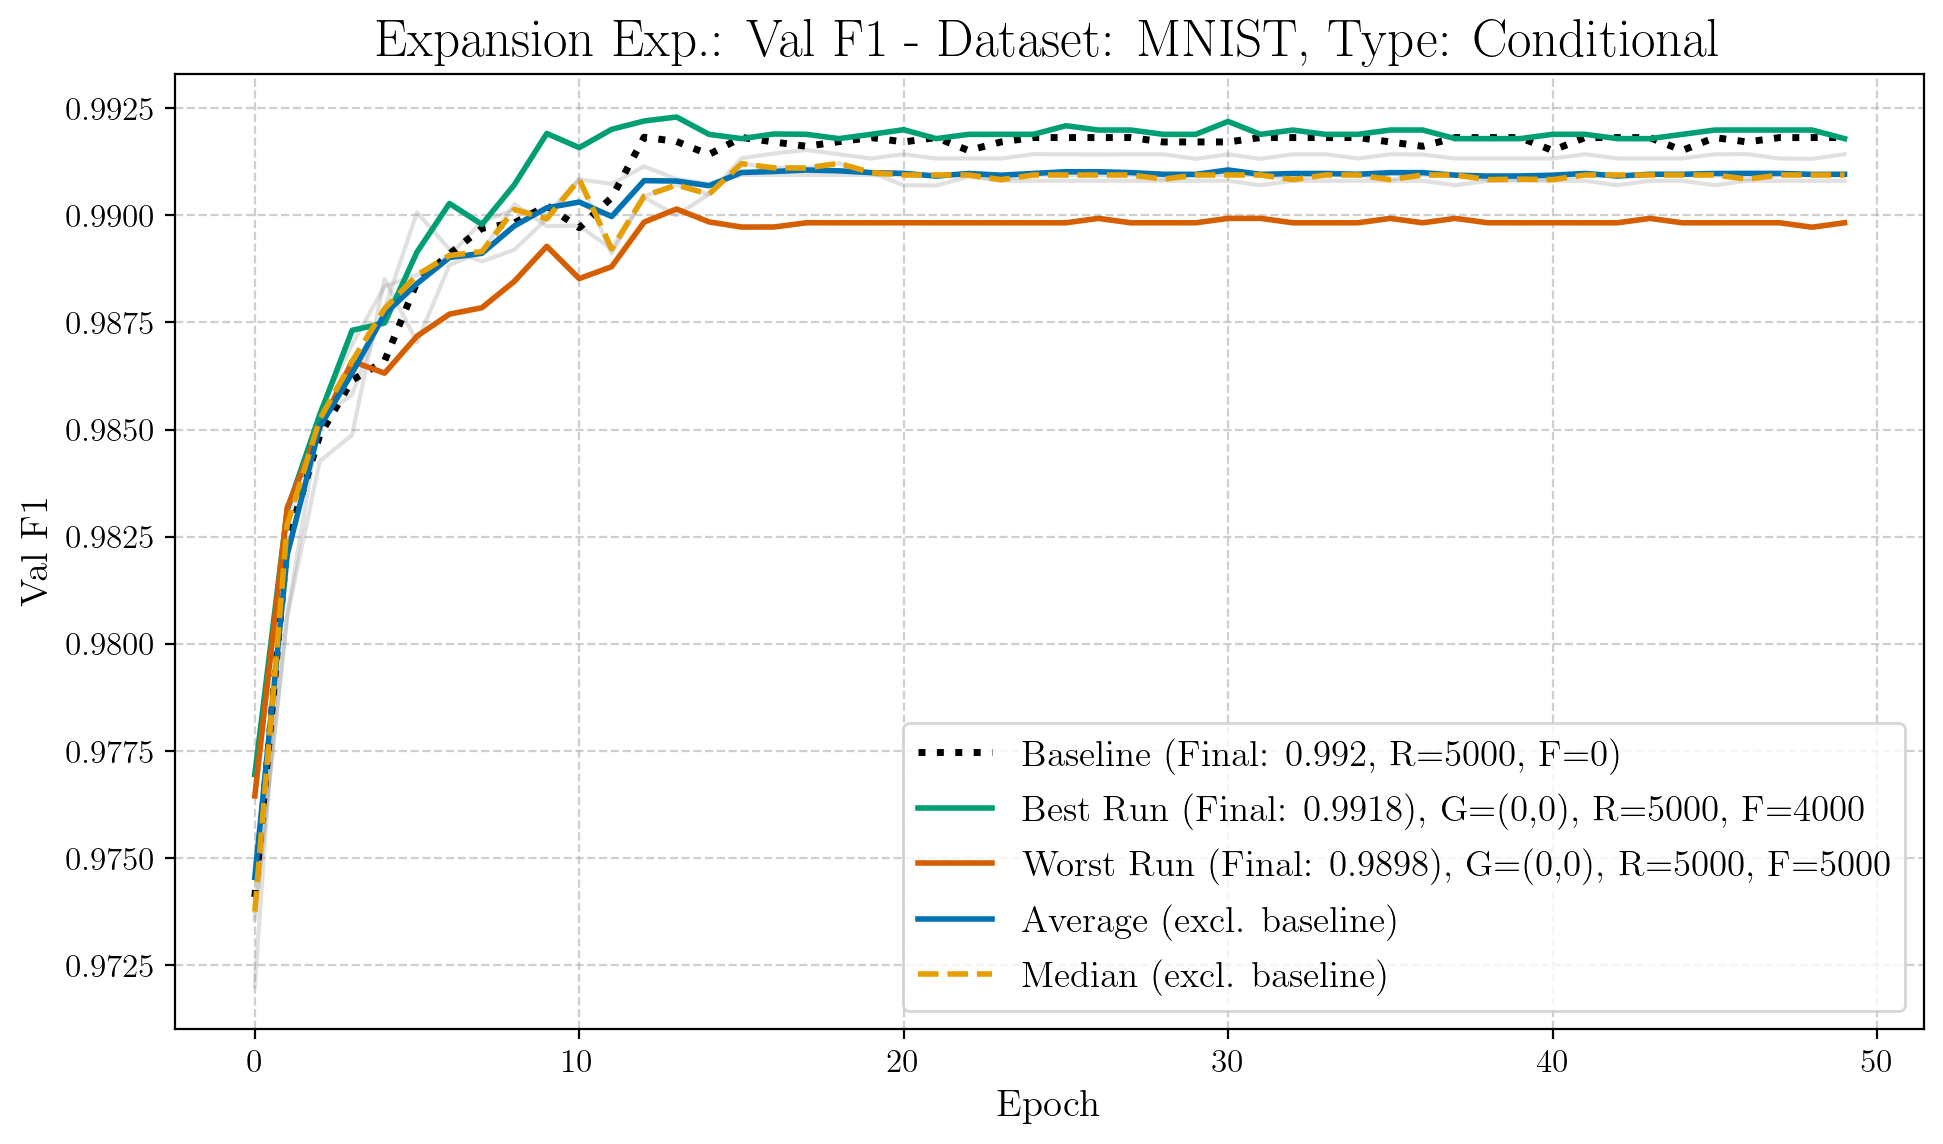
\includegraphics[width=.85\textwidth]{abb/strat_classifier_performance/MNIST_STRATIFIED_CLASSIFIERS_COND_GAN/expansion_experiments/val_f1_score_['COND']_MNIST_all.png}
	\label{fig:app_strat_class_performance_expansion_exp._val_f1_score_cGAN}
\end{figure}
\begin{table}[H]
	\centering
	\vspace{-1em}
	\begin{tabular}{|c|c|c|c|c|}
		\hline
		Run Type & Experiment & Val F1 \\ \hline
		best & Conditional (R:5000, F:4000) & $0.9918$\\ \hline
		worst & Conditional (R:5000, F:5000) & $0.9898$\\ \hline
		median & Conditional & $0.9909$\\ \hline
		average & Conditional & $0.9910$
		\\ \hline
	\end{tabular}
\end{table}
% End LaTeX Table for Expansion Experiment:
% LaTeX Metrics Table for Replacement Experiment: - Metric: val_f1_score
% LaTeX Metrics Table for Replacement Experiment: - Metric: val_f1_score - Target Gen Group: 10
\noindent\textbf{Replacement Experiment:}
\begin{figure}[htbp]
	\centering
	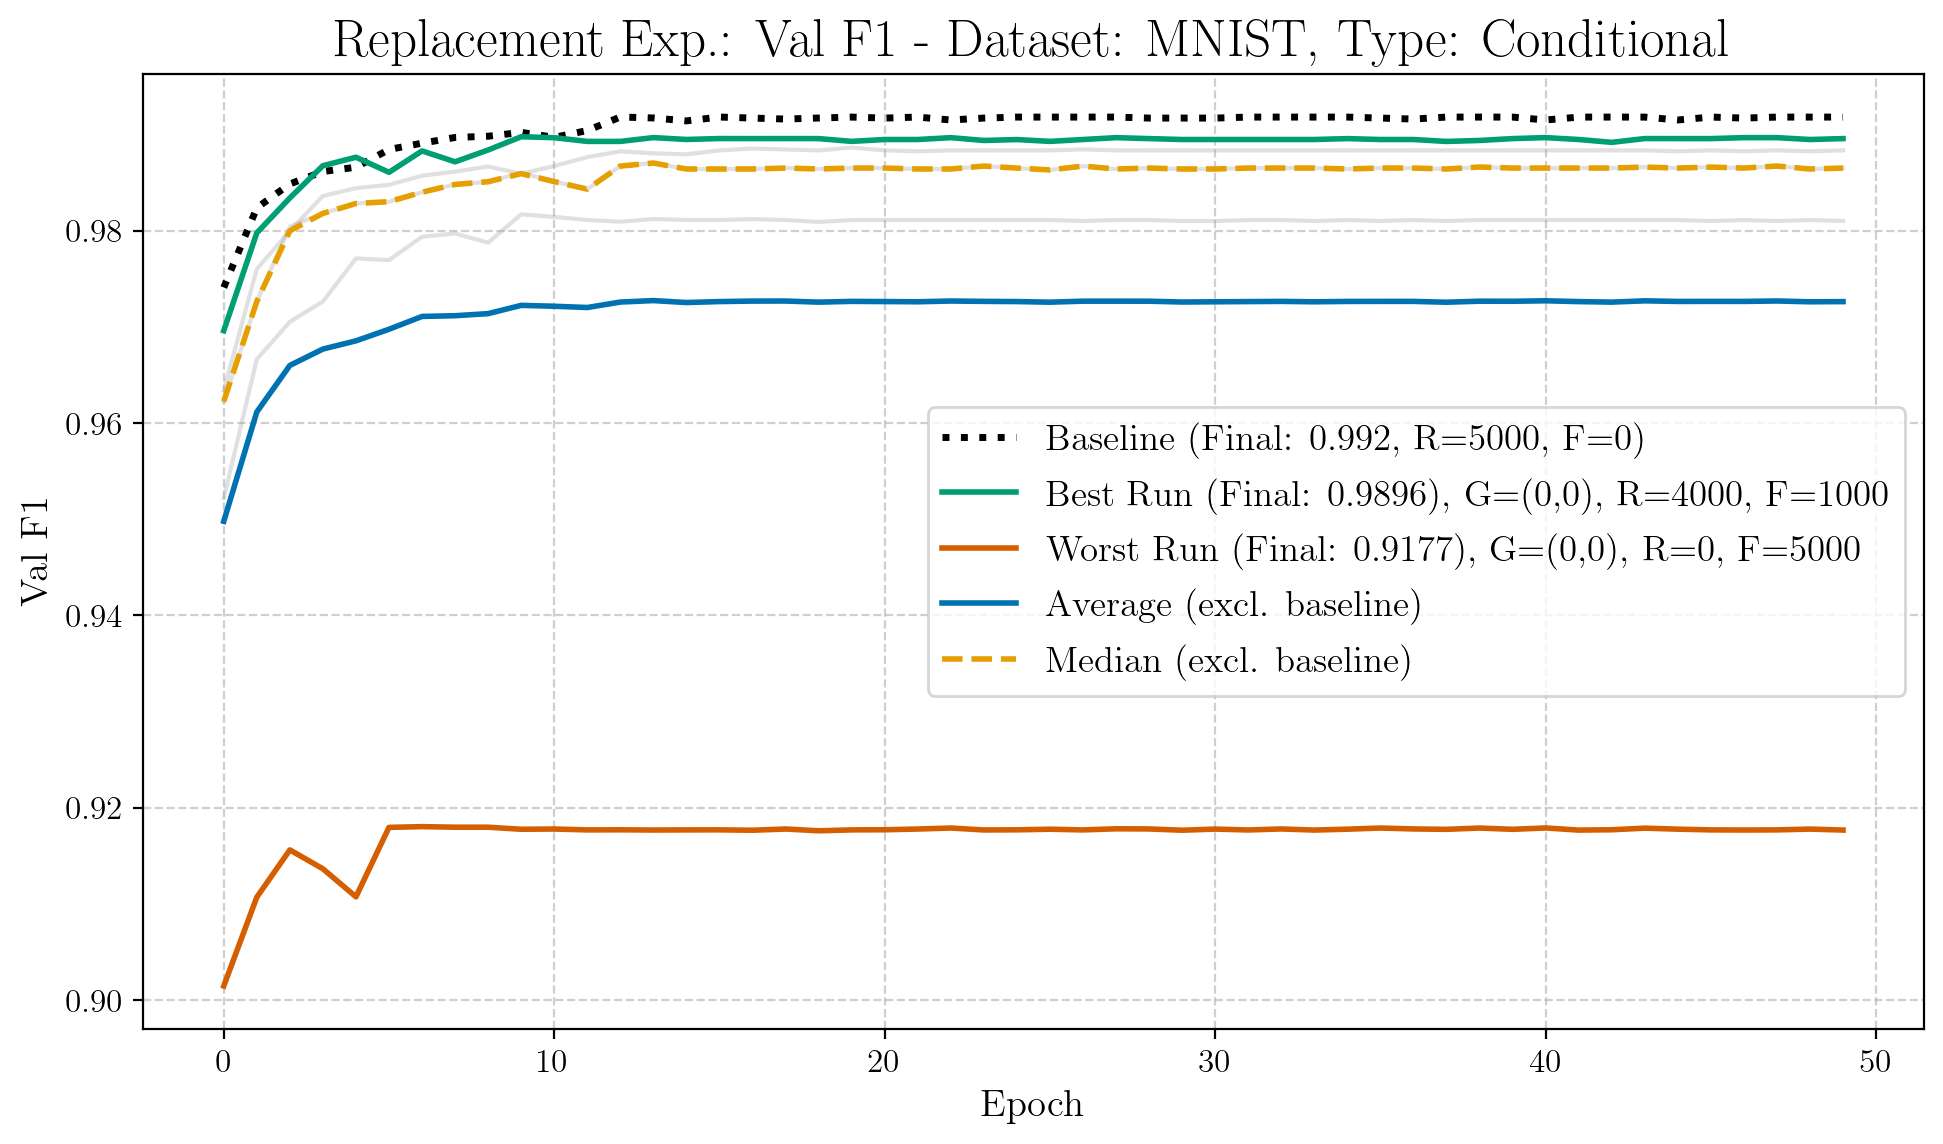
\includegraphics[width=.85\textwidth]{abb/strat_classifier_performance/MNIST_STRATIFIED_CLASSIFIERS_COND_GAN/replacement_experiments/val_f1_score_['COND']_MNIST_all.png}
	\label{fig:app_strat_class_performance_replacement_exp._val_f1_score_cGAN}
\end{figure}
\begin{table}[H]
	\centering
	\vspace{-1em}
	\begin{tabular}{|c|c|c|c|c|}
		\hline
		Run Type & Experiment & Val F1 \\ \hline
		best & Conditional (R:4000, F:1000) & $0.9896$\\ \hline
		worst & Conditional (R:0, F:5000) & $0.9177$\\ \hline
		median & Conditional & $0.9865$\\ \hline
		average & Conditional & $0.9726$
		\\ \hline
	\end{tabular}
\end{table}
% End LaTeX Table for Replacement Experiment:
\newpage
\subsubsection{Dataset: FASHION, Architecture: DCGAN}
% LaTeX Metrics Table for Expansion Experiment: - Metric: val_f1_score
% LaTeX Metrics Table for Expansion Experiment: - Metric: val_f1_score - Target Gen Group: 10
\noindent\textbf{Expansion Experiment:}
\begin{figure}[htbp]
	\centering
	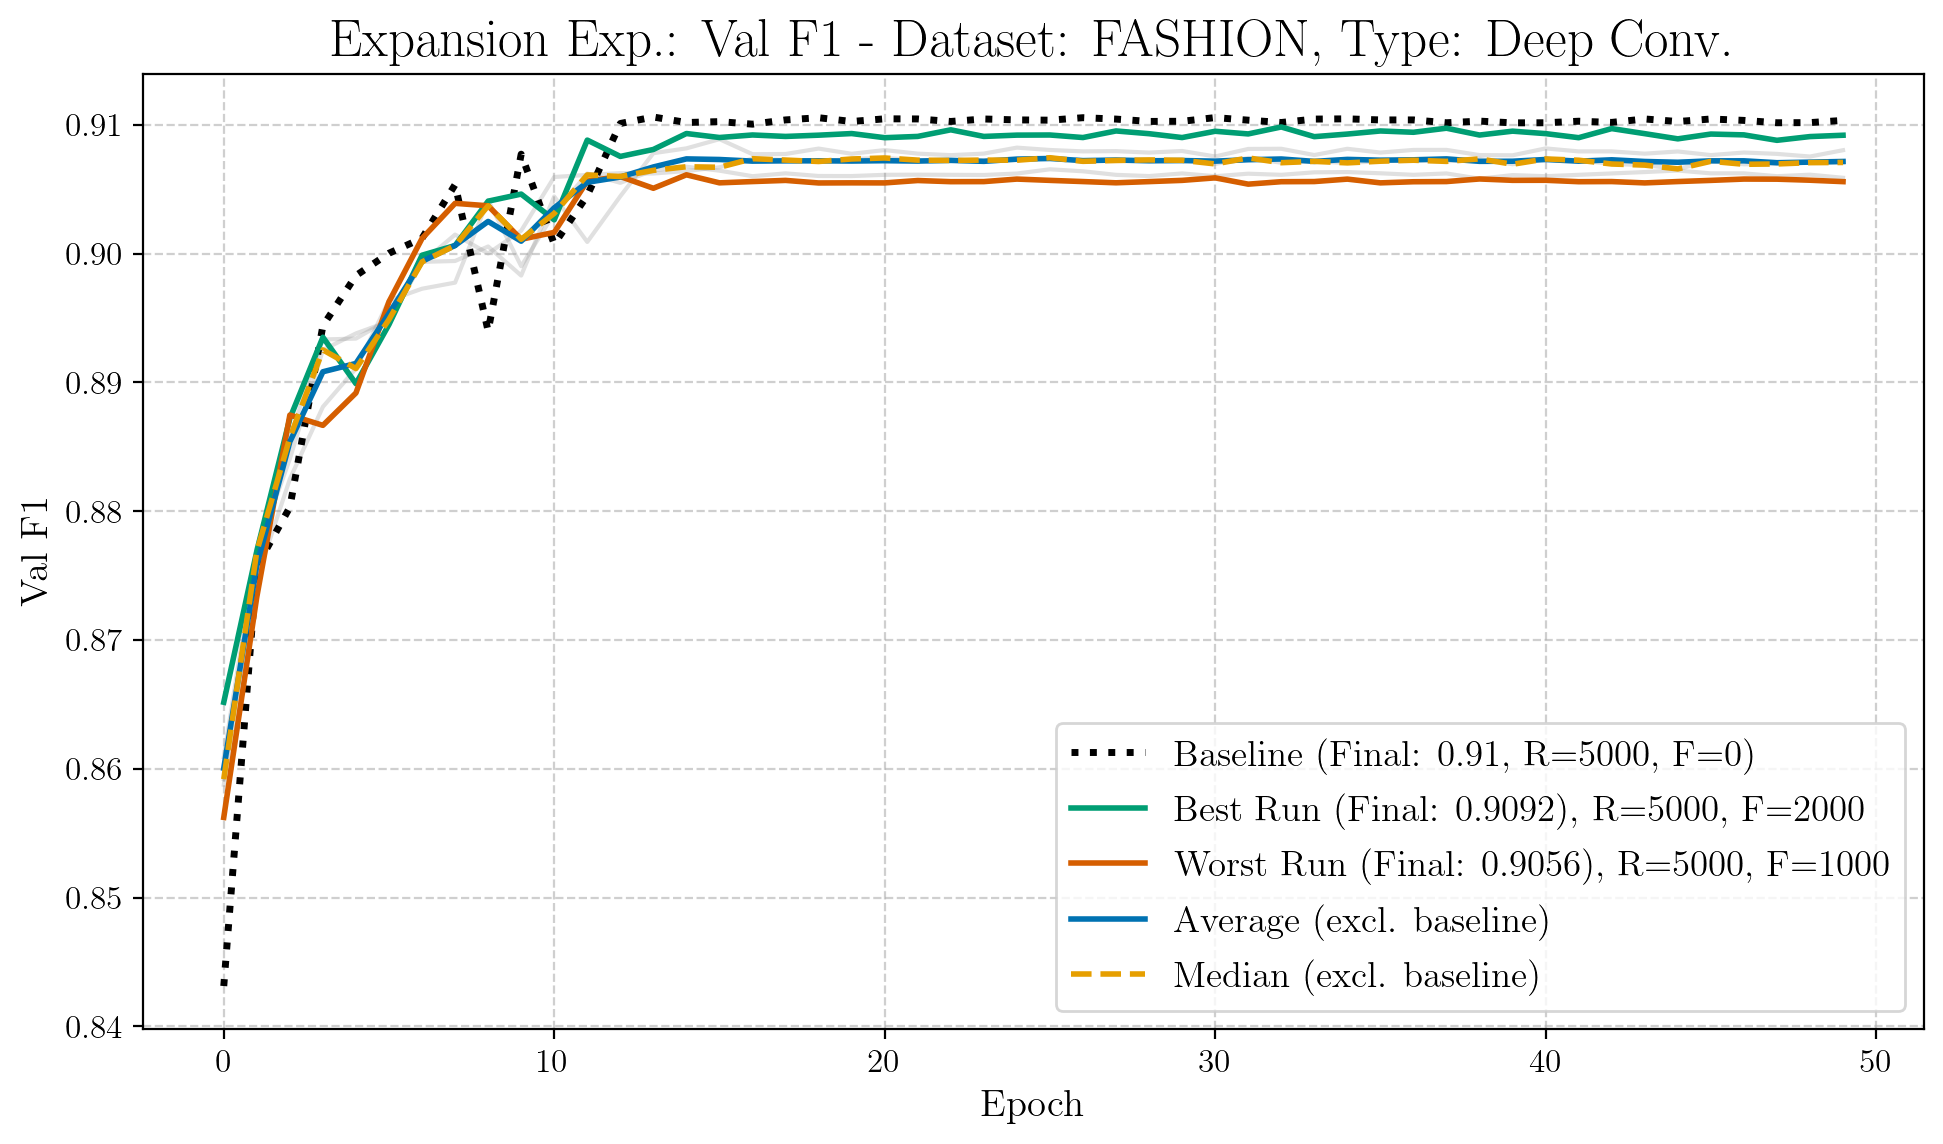
\includegraphics[width=.85\textwidth]{abb/strat_classifier_performance/FASHION_STRATIFIED_CLASSIFIERS_VANILLA_GAN/expansion_experiments/val_f1_score_['VANILLA']_FASHION_all.png}
	\label{fig:app_strat_class_performance_expansion_exp._val_f1_score_}
\end{figure}
\begin{table}[H]
	\centering
	\vspace{-1em}
	\begin{tabular}{|c|c|c|c|c|}
		\hline
		Run Type & Experiment & Performance \\ \hline
		best & DC (R:5000, F:2000) & $0.9092$\\ \hline
		worst & DC (R:5000, F:1000) & $0.9056$\\ \hline
		median & DC & $0.9071$\\ \hline
		average & DC & $0.9072$
		\\ \hline
	\end{tabular}
\end{table}
% End LaTeX Table for Expansion Experiment:
% LaTeX Metrics Table for Replacement Experiment: - Metric: val_f1_score
% LaTeX Metrics Table for Replacement Experiment: - Metric: val_f1_score - Target Gen Group: 10
\noindent\textbf{Replacement Experiment:}
\begin{figure}[htbp]
	\centering
	\includegraphics[width=.85\textwidth]{abb/strat_classifier_performance/FASHION_STRATIFIED_CLASSIFIERS_VANILLA_GAN/replacement_experiments/val_f1_score_['VANILLA']_FASHION_all.png}
	\label{fig:app_strat_class_performance_replacement_exp._val_f1_score_}
\end{figure}
\begin{table}[H]
	\centering
	\vspace{-1em}
	\begin{tabular}{|c|c|c|c|c|}
		\hline
		Run Type & Experiment & Performance \\ \hline
		best & DC (R:5000, F:1000) & $0.9046$\\ \hline
		worst & DC (R:0, F:5000) & $0.8470$\\ \hline
		median & DC & $0.8897$\\ \hline
		average & DC & $0.8823$
		\\ \hline
	\end{tabular}
\end{table}
% End LaTeX Table for Replacement Experiment:
\newpage
\subsubsection{Dataset: FASHION, Architecture: COND GAN}
% LaTeX Metrics Table for Expansion Experiment: - Metric: val_f1_score
% LaTeX Metrics Table for Expansion Experiment: - Metric: val_f1_score - Target Gen Group: 10
\noindent\textbf{Expansion Experiment:}
\begin{figure}[htbp]
	\centering
	\includegraphics[width=.85\textwidth]{abb/strat_classifier_performance/FASHION_STRATIFIED_CLASSIFIERS_COND_GAN/expansion_experiments/val_f1_score_['COND']_FASHION_all.png}
	\label{fig:app_strat_class_performance_expansion_exp._val_f1_score_}
\end{figure}
\begin{table}[H]
	\centering
	\vspace{-1em}
	\begin{tabular}{|c|c|c|c|c|}
		\hline
		Run Type & Experiment & Val F1 \\ \hline
		best & Conditional (R:5000, F:1000) & $0.9123$\\ \hline
		worst & Conditional (R:5000, F:3000) & $0.9060$\\ \hline
		median & Conditional & $0.9085$\\ \hline
		average & Conditional & $0.9089$
		\\ \hline
	\end{tabular}
\end{table}
% End LaTeX Table for Expansion Experiment:
% LaTeX Metrics Table for Replacement Experiment: - Metric: val_f1_score
% LaTeX Metrics Table for Replacement Experiment: - Metric: val_f1_score - Target Gen Group: 10
\noindent\textbf{Replacement Experiment:}
\begin{figure}[htbp]
	\centering
	\includegraphics[width=.85\textwidth]{abb/strat_classifier_performance/FASHION_STRATIFIED_CLASSIFIERS_COND_GAN/replacement_experiments/val_f1_score_['COND']_FASHION_all.png}
	\label{fig:app_strat_class_performance_replacement_exp._val_f1_score_}
\end{figure}
\begin{table}[H]
	\centering
	\vspace{-1em}
	\begin{tabular}{|c|c|c|c|c|}
		\hline
		Run Type & Experiment & Val F1 \\ \hline
		best & Conditional (R:4000, F:1000) & $0.9023$\\ \hline
		worst & Conditional (R:0, F:5000) & $0.5962$\\ \hline
		median & Conditional & $0.8923$\\ \hline
		average & Conditional & $0.8427$
		\\ \hline
	\end{tabular}
\end{table}
% End LaTeX Table for Replacement Experiment:
\newpage

\subsubsection{Dataset: MNIST, Architecture: TDA}
% LaTeX Metrics Table for Expansion Experiment: - Metric: val_f1_score
% LaTeX Metrics Table for Expansion Experiment: - Metric: val_f1_score - Target Gen Group: 10
\noindent\textbf{Expansion Experiment:}
\begin{figure}[htbp]
	\centering
	\includegraphics[width=.85\textwidth]{abb/strat_classifier_performance/tda_mnist/expansion_experiments/val_f1_score_tda_mnist_mnist_all.png}
	\label{fig:app_strat_class_performance_expansion_exp._val_f1_score_}
\end{figure}
\begin{table}[H]
	\centering
	\vspace{-1em}
	\begin{tabular}{|c|c|c|c|c|}
		\hline
		Run Type & Metric & Val F1 \\ \hline
		best & TDA (R:5000, F:2000) & $0.9938$\\ \hline
		worst & TDA (R:5000, F: 1000) & $0.9923$\\ \hline
		median & TDA & $0.9934$\\ \hline
		average & TDA & $0.9932$
		\\ \hline
	\end{tabular}
\end{table}
% End LaTeX Table for Expansion Experiment:
% LaTeX Metrics Table for Replacement Experiment: - Metric: val_f1_score
% LaTeX Metrics Table for Replacement Experiment: - Metric: val_f1_score - Target Gen Group: 10
\noindent\textbf{Replacement Experiment:}
\begin{figure}[htbp]
	\centering
	\includegraphics[width=.85\textwidth]{abb/strat_classifier_performance/tda_mnist/replacement_experiments/val_f1_score_tda_mnist_mnist_all.png}
	\label{fig:app_strat_class_performance_replacement_exp._val_f1_score_}
\end{figure}
\begin{table}[H]
	\centering
	\vspace{-1em}
	\begin{tabular}{|c|c|c|c|c|}
		\hline
		Run Type & Experiment & Performance \\ \hline
		best & TDA (R:3000, F:2000) & $0.9922$\\ \hline
		worst & TDA (R:0, F:5000) & $0.9905$\\ \hline
		median & TDA & $0.9917$\\ \hline
		average & TDA & $0.9914$
		\\ \hline
	\end{tabular}
\end{table}
% End LaTeX Table for Replacement Experiment:
\newpage
\subsubsection{Dataset: FASHION, Architecture: TDA}
% LaTeX Metrics Table for Expansion Experiment: - Metric: val_f1_score
% LaTeX Metrics Table for Expansion Experiment: - Metric: val_f1_score - Target Gen Group: 10
\noindent\textbf{Expansion Experiment:}
\begin{figure}[htbp]
	\centering
	\includegraphics[width=.85\textwidth]{abb/strat_classifier_performance/tda_fashion_mnist/expansion_experiments/val_f1_score_tda_fashion_mnist_fashion_all.png}
	\label{fig:app_strat_class_performance_expansion_exp._val_f1_score_}
\end{figure}
\begin{table}[H]
	\centering
	\vspace{-1em}
	\begin{tabular}{|c|c|c|c|c|}
		\hline
		Run Type & Experiment & Val F1 \\ \hline
		best & TDA (R:5000, F:4000) & $0.9129$\\ \hline
		worst & TDA (R:5000, F:5000) & $0.9108$\\ \hline
		median & TDA & $0.9119$\\ \hline
		average & TDA & $0.9118$
		\\ \hline
	\end{tabular}
\end{table}
% End LaTeX Table for Expansion Experiment:
% LaTeX Metrics Table for Replacement Experiment: - Metric: val_f1_score
% LaTeX Metrics Table for Replacement Experiment: - Metric: val_f1_score - Target Gen Group: 10
\noindent\textbf{Replacement Experiment:}
\begin{figure}[htbp]
	\centering
	\includegraphics[width=.85\textwidth]{abb/strat_classifier_performance/tda_fashion_mnist/replacement_experiments/val_f1_score_tda_fashion_mnist_fashion_all.png}
	\label{fig:app_strat_class_performance_replacement_exp._val_f1_score_}
\end{figure}
\begin{table}[H]
	\centering
	\vspace{-1em}
	\begin{tabular}{|c|c|c|c|c|}
		\hline
		Run Type & Experiment & Val F1 \\ \hline
		best & TDA (R:3000, F:2000) & $0.9048$\\ \hline
		worst & TDA (R:0, F:5000) & $0.8874$\\ \hline
		median & TDA & $0.8934$\\ \hline
		average & TDA & $0.8955$
		\\ \hline
	\end{tabular}
\end{table}
% End LaTeX Table for Replacement Experiment:
\newpage

\subsection{Data Creation Histograms}
\subsubsection{DCGAN MNIST}

\begin{figure}[htbp]
    \centering
    \includegraphics[width=.9\textwidth]{abb/datageneration_histograms/dc_mnist.png}
    \caption{A histogram chart depicting the class distribution of the generated data with the DCGAN generator trained on the \textbf{MNIST} dataset. The labels result from an auxiliary classifier as mentioned in \ref{body_experiment_labeling_data}.}
    \label{fig:figure_dcgan_datacreation_histogram}
\end{figure}
